\section{Notation and Deferred Proofs}
\label{app:proof}

\subsection{Notation and scope}
The population parameter $\theta$ is scalar; the LoRA parameter vector uses
the same symbol but belongs to a fixed shared coordinate space. The population
constants $a,b$ are correct- and incorrect-acceptance probabilities, and $b$
also fixes the high-magnitude group mass in this particular construction.
$p_s=\sigma(s\theta)$, $\rho_1=1-b$, $\rho_L=b$, and
$D=1-P=(1-b)(1-p_1)+b(1-p_L)$.
Population flow time is denoted by $t$ and audit probability by $q$.
Finite-pool quantities $K,C,E$ are counts, not population probabilities.
$g_i$ denotes an unscaled per-response gradient, $G_v$ its selected-pool mean,
$h$ the unnormalized reference-loss gradient, and $\delta_v$ an actual
optimizer parameter change. All norms below are Euclidean in the specified
coordinates. The proofs concern exact arithmetic; implementation residuals
are reported separately. Population convergence is not a claim about finite
Euler steps, AdamW, greedy decoding, or the language-model experiments.

The population arguments first establish validity of the acceptance rules
and derive the supervised gradient at a frozen sampling parameter. We then
prove regularity of the resulting vector fields before analyzing their
trajectories. The auditing argument repeats both the normalization and the
sign analysis after removal of audited errors. The final proofs concern
finite-pool gradients and reference loss, not population sampling accuracy.

\subsection{Proof of Lemma~\ref{lem:influence}}
\begin{proof}
\textit{Step 1: common normalization.}
All probabilities and expectations in this proof are taken under the common
learner $\theta_0$. Since $0<P_0<1$, both correctness-conditional
distributions are defined. Total probability gives, for either $v\in\{R,S\}$,
\begin{align*}
 \mathbb E[A_v]
 &=P_0\mathbb E[A_v\mid c=1]+(1-P_0)\mathbb E[A_v\mid c=0]\\
 &=P_0t+(1-P_0)f=Z.
\end{align*}
Similarly, $\mathbb E[A_v c]=tP_0$, and therefore
$\Pr(c=1\mid A_v=1)=tP_0/Z$. Both yield and accepted-data precision are
common without adding either as an independent matching assumption.

\textit{Step 2: subtract the stopped gradients.}
A sufficient condition for exchanging differentiation and expectation is
that $\ell(\theta_0;x,y)$ is integrable, $\ell(\cdot;x,y)$ is differentiable
on a neighborhood of $\theta_0$, and
$\sup_{\vartheta}\|\nabla_\vartheta\ell(\vartheta;x,y)\|$
over that neighborhood is bounded by an integrable function.
Since $0\leq A_v\leq1$ and acceptance is held fixed, the same bound
dominates the accepted loss's difference quotients. Dominated convergence
then gives the gradient formula below coordinate by coordinate.
The finite-support logistic construction satisfies these conditions:
its loss is finite at $\theta_0$ and
$|\partial_\vartheta\ell(\vartheta;x,y)|\leq|x|\leq L$.
Realize both acceptance decisions on the same probability space as $(x,y)$,
for example using conditionally independent auxiliary random seeds. This
coupling is only a device for writing a difference; the two rules need not
accept the same responses. The assumed exchange of differentiation and
expectation, with $Z$ held fixed under $\nabla_\vartheta$, gives
\begin{equation}
 G_v=\frac{\mathbb E[A_v g]}{Z},\qquad
 G_S-G_R=\frac{\mathbb E[Ug]}{Z},\qquad U=A_S-A_R.
 \label{eq:app-gradient-difference}
\end{equation}
Since $|U|\leq1$ and $g$ is integrable, $Ug$ and the conditional
expectations below are integrable componentwise. No second moment of $g$
is needed.

\textit{Step 3: condition on correctness.}
Matched rates imply
\[
 \mathbb E[U\mid c=1]=t-t=0,\qquad
 \mathbb E[U\mid c=0]=f-f=0.
\]
For each coordinate $g_j$ and each $k\in\{0,1\}$, conditional covariance
therefore satisfies
\begin{align*}
 \operatorname{Cov}(U,g_j\mid c=k)
 &=\mathbb E[Ug_j\mid c=k]
   -\mathbb E[U\mid c=k]\mathbb E[g_j\mid c=k]\\
 &=\mathbb E[Ug_j\mid c=k].
\end{align*}
Total expectation in~\eqref{eq:app-gradient-difference} proves
\eqref{eq:influence-gap} coordinate by coordinate. The expression does not
depend on the coupling because its product expectation equals
$\mathbb E[A_Sg\mid c=k]-\mathbb E[A_Rg\mid c=k]$. The identity does not
assert that these covariances are nonzero; it identifies the moments left
unconstrained by rate matching.
\end{proof}

\subsection{Proof of Lemma~\ref{lem:piecewise}}
\begin{proof}
\textit{Step 1: identify which group exhausts the error quota.}
At finite $\theta$, $0<p_s<1$, hence $m_1,m_L>0$ and $D=m_1+m_L>0$.
The switching condition is exactly
\begin{equation}
 Q-m_L=b(1-b)(p_L-p_1).
 \label{eq:app-quota-switch}
\end{equation}
Since $L>1$ and $\sigma$ is strictly increasing, $p_L-p_1$ has the sign of
$\theta$. For $\theta\leq0$, $Q\leq m_L$, so the definition of $S$ gives
\[
 r_{S,1}=0,\qquad r_{S,L}=\frac{Q}{m_L}=\frac{D}{1-p_L}.
\]
Here $D$ is a convex combination of two positive numbers, each at most
$1-p_L$, so $0<r_{S,L}\leq1$. For $\theta\geq0$, $Q\geq m_L$, whence
\[
 r_{S,L}=1,\qquad r_{S,1}=\frac{Q-m_L}{m_1}
                         =\frac{b(p_L-p_1)}{1-p_1}.
\]
Since $0\leq p_L-p_1\leq1-p_1$, this last rate lies in $[0,b]$.
At $\theta=0$, $p_1=p_L=D=1/2$, so both expressions give
$(r_{S,1},r_{S,L})=(0,1)$. In particular, the switch is continuous.

\textit{Step 2: verify the operating rates and denominator.}
If $Q\leq m_L$, the accepted-error mass is
$m_L(Q/m_L)+m_1\cdot0=Q$; if $Q\geq m_L$, it is
$m_L\cdot1+m_1[(Q-m_L)/m_1]=Q$. Thus
\[
 \Pr(A_S=1,c=0)=Q=bD,
 \qquad \Pr(A_S=1\mid c=0)=\frac{bD}{D}=b.
\]
The random rule has the same accepted-error mass $\sum_s m_s b=bD$.
Both rules accept each correct candidate with probability $a$, so the
accepted-correct mass is $aP$ and TPR is $a$. Consequently $Z=aP+bD>0$
and $\pi=aP/Z$ for either rule, at the common parameter.

\textit{Step 3: differentiate the loss, not the sampling law.}
For a fixed candidate $\hat y\in\{0,1\}$, binary cross entropy is
\[
 \ell(\vartheta;x,\hat y)
 =-\hat y\log\sigma(\vartheta x)
   -(1-\hat y)\log[1-\sigma(\vartheta x)],
 \qquad \partial_\vartheta\ell=(\sigma(\vartheta x)-\hat y)x.
\]
For $x=s$, a correct response $\hat y=1$ has derivative $-s(1-p_s)$ at
$\vartheta=\theta$, and an error $\hat y=0$ has derivative $sp_s$.
For $x=-s$, $\sigma(-s\theta)=1-p_s$: the correct response $\hat y=0$
has derivative $(1-p_s)(-s)=-s(1-p_s)$, and the error $\hat y=1$ has
derivative $(-p_s)(-s)=sp_s$. Both signs therefore have the same
correctness probabilities and gradient contributions.

Conditioning on magnitude and summing over its two signs gives
\begin{align}
 N_v(\theta)
 &=\sum_s\rho_s\left\{a p_s[-s(1-p_s)]
            +r_{v,s}(1-p_s)[sp_s]\right\}\nonumber\\
 &=\sum_s\rho_s s p_s(1-p_s)(r_{v,s}-a).
 \label{eq:app-numerator}
\end{align}
Dividing by the yield proves~\eqref{eq:logistic-gradient}. This is
$\partial_\vartheta\mathcal L_v(\vartheta;\theta)|_{\vartheta=\theta}$,
not the total derivative of $\mathcal L_v(\theta;\theta)$. Candidate
probabilities, acceptance probabilities, and $Z$ are fixed under
$\partial_\vartheta$. Recomputing them at a new parameter defines the next
vector-field value, not additional terms in this derivative.

For later use, differentiation of the evaluation quantity alone gives
\[
 P'(\theta)=(1-b)p_1(1-p_1)+bL p_L(1-p_L)>0.
\]
Thus $P(0)=1/2$, $P$ is strictly increasing, and its limits at $-\infty$
and $+\infty$ are respectively zero and one. At $L=1$, the two named
groups give $Q=m_L$ at every parameter, so $(r_{S,1},r_{S,L})=(0,1)$;
the gradient derivation still applies to that ablation.
\end{proof}

\subsection{Proof of Proposition~\ref{prop:separation}}
\begin{proof}
\textit{Step 1: compute the gradient exactly.}
At $\theta_0=0$,
\[
 p_1=p_L=\frac12,\quad m_1=\frac{1-b}{2},\quad m_L=\frac b2,
 \quad D=\frac12,\quad Q=\frac b2=m_L.
\]
Thus $r_{S,1}=0$, $r_{S,L}=1$, and $Z(0)=(a+b)/2$.
Equation~\eqref{eq:app-numerator} yields
\begin{align*}
 N_R(0)&=\frac{(b-a)(1-b+bL)}4=\frac{(b-a)\bar s}{4},\\
 N_S(0)&=\frac{-a(1-b)+bL(1-a)}4=\frac{bL-a\bar s}{4},
 \qquad\bar s=1-b+bL.
\end{align*}
Division by $Z(0)$ proves~\eqref{eq:general-initial}.

\textit{Step 2: relate signs to the finite update.}
For $\eta>0$, $\theta_v^+=-\eta g_v(0)$. Strict monotonicity of $P$ gives
\[
 P(\theta_v^+)>\frac12\ \Longleftrightarrow\ g_v(0)<0,
 \qquad P(\theta_v^+)<\frac12\ \Longleftrightarrow\ g_v(0)>0.
\]
These are exact equivalences, not small-step approximations. Since $b<a$
and $\bar s>0$, $R$ improves for every $\eta>0$. Since $b(1-a)>0$,
\[
 g_S(0)>0\ \Longleftrightarrow\ bL(1-a)>a(1-b)
          \ \Longleftrightarrow\ L>\frac{a(1-b)}{b(1-a)}.
\]
At equality the $S$ update is zero; below the threshold its accuracy
increases. The threshold exceeds one because
$a(1-b)>b(1-a)$ is equivalent to $a>b$.

\textit{Step 3: specialize the example.}
For $a=3/4$, $b=1/2$, we have $\bar s=(1+L)/2$ and
\[
 g_R(0)=-\frac{L+1}{20},\quad g_S(0)=\frac{L-3}{20},\quad
 Z(0)=\frac58,\quad \pi(0)=\frac{(3/4)(1/2)}{5/8}=\frac35.
\]
TPR and FPR are respectively $3/4$ and $1/2$ by Lemma~\ref{lem:piecewise}.
This proves all matched-summary assertions and the strict separation
when $L>3$.
\end{proof}

\subsection{Auxiliary flow lemmas}
\begin{lemma}[Regularity of the accepted-gradient fields]
\label{lem:flow-regularity}
Fix $0<b<a<1$ and finite $L>1$. The fields $g_R,g_S$ and the group-audited
field $g_{S,q}$ for every fixed $q\in[0,1]$ are locally Lipschitz on
$\mathbb R$ and satisfy $|g(\theta)|\leq L$. Their autonomous flows have
unique solutions for all $t\geq0$, from any finite initial parameter.
\end{lemma}
\begin{proof}
\textit{Local Lipschitz continuity.}
On each compact parameter interval $I$, the smooth functions $1-p_1$ and
$1-p_L$ have positive minima. Thus $m_1,m_L$ are bounded away from zero
on $I$, and $Q/m_L$ and $(Q-m_L)/m_1$ are smooth there. The maps
$u\mapsto\min\{1,u\}$ and $u\mapsto\max\{0,u\}$ are 1-Lipschitz;
their compositions define locally Lipschitz acceptance rates, including
at $\theta=0$, where differentiability need not hold. Products and sums in
\eqref{eq:app-numerator} are therefore locally Lipschitz. The unaudited
denominator satisfies
\[
 Z(\theta)=aP+b(1-P)\geq\min\{a,b\}>0.
\]
After an audit, the effective error rates are $r_{S,1}$ and
$(1-q)r_{S,L}$, and
\[
 Z_q(\theta)=aP+(1-b)(1-p_1)r_{S,1}
                   +b(1-p_L)(1-q)r_{S,L}\geq aP(\theta)>0.
\]
On $I$ this bound is at least $a\min_I P>0$. Taking reciprocals thus
preserves local Lipschitz continuity, proving the assertion for each
normalized field. This includes $q=1$; no global lower bound on $Z_q$
is needed.

\textit{Bound independent of the yield.}
Each candidate derivative is $(\sigma(\theta x)-\hat y)x$, with absolute
value at most $|x|\leq L$. If $A$ is its final retention indicator,
including audit removal, write
$\xi=\partial_\vartheta\ell(\vartheta;x,\hat y)|_{\vartheta=\theta}$. Then
\[
 |g(\theta)|
 =\left|\frac{\mathbb E[A\xi]}{\mathbb E[A]}\right|
 \leq\frac{\mathbb E[A|\xi|]}{\mathbb E[A]}\leq L.
\]
This conditional-average bound remains valid when yield becomes small.

\textit{Global continuation.}
Local Lipschitz continuity gives a unique local solution. If its maximal
forward existence time $T$ were finite, boundedness would imply
\[
 |\theta(t)-\theta(u)|\leq L|t-u|\qquad(0\leq u,t<T).
\]
The trajectory would then have a finite limit as $t\uparrow T$ and stay
in a compact interval. Local existence at that limit extends it beyond
$T$, a contradiction. Thus $T=\infty$. Uniqueness follows from local
uniqueness on overlapping time intervals.
\end{proof}

\begin{lemma}[The first equilibrium blocks a harmful flow]
\label{lem:scalar-flow}
Let $g:\mathbb R\to\mathbb R$ be bounded and locally Lipschitz, with
$g(0)>0$ and $g(\theta)<0$ for every sufficiently negative $\theta$.
Then the solution of $\dot\theta=-g(\theta)$, $\theta(0)=0$, exists uniquely
for all nonnegative time and strictly decreases to the largest negative
zero $\theta_*$ of $g$.
\end{lemma}
\begin{proof}
\textit{Step 1: existence of a largest negative zero.}
Choose $u_0<0$ so that $g(\theta)<0$ for all $\theta\leq u_0$.
Continuity and $g(0)>0$ give an $\varepsilon>0$ with
$-\varepsilon>u_0$ such that $g$ is positive on $[-\varepsilon,0]$.
The intermediate value theorem gives a zero between $u_0$ and zero.
All negative zeros lie in $[u_0,-\varepsilon]$, and the zero set is closed
by continuity. It is therefore nonempty and compact and has a maximum
$\theta_*<0$. There are no zeros on $(\theta_*,0]$; continuity and
$g(0)>0$ imply $g>0$ throughout that interval.

\textit{Step 2: global existence and no finite-time arrival.}
Boundedness and local Lipschitz continuity give global existence and
uniqueness by the continuation argument in Lemma~\ref{lem:flow-regularity},
using a bound for $g$ in place of $L$. While $\theta(t)\in(\theta_*,0]$,
its derivative is $-g(\theta(t))<0$. To rule out arrival at the lower
endpoint, take a finite Lipschitz constant $K_*$ for $g$ on $[\theta_*,0]$.
Such a constant exists by local Lipschitz continuity, a finite cover of
the compact interval, and subdivision between two arbitrary points.
Since $g(\theta_*)=0$,
\[
 0<g(\theta)\leq K_*(\theta-\theta_*)
 \qquad(\theta_*<\theta\leq0).
\]
Before any proposed first hitting time, $d(t)=\theta(t)-\theta_*$ satisfies
$\dot d\geq-K_*d$. Hence
$\frac{d}{dt}[e^{K_*t}d(t)]\geq0$, giving
\begin{equation}
 \theta(t)-\theta_*\geq(-\theta_*)e^{-K_*t}>0.
 \label{eq:app-nonhitting}
\end{equation}
By continuity this rules out a finite first hit. A crossing would require
a hit, so it is excluded as well. Thus the trajectory stays in
$(\theta_*,0]$ and strictly decreases at every finite time.

\textit{Step 3: identify the monotone limit.}
Monotonicity and the lower bound give a finite limit
$\ell=\lim_{t\to\infty}\theta(t)\in[\theta_*,0]$. If $\ell>\theta_*$,
then $g(\ell)>0$, and continuity gives $g\geq\gamma>0$ near $\ell$.
For all sufficiently large $t$, integrating $\dot\theta\leq-\gamma$
would force $\theta(t)\to-\infty$, contrary to its lower bound. Therefore
$\ell=\theta_*$. Neither simplicity of this zero nor uniqueness of other
equilibria is needed. The bound~\eqref{eq:app-nonhitting} is a lower bound
on distance to equilibrium, not an exponential convergence-rate guarantee.
\end{proof}

\subsection{Proof of Theorem~\ref{thm:flow}}
\begin{proof}
\textit{Step 1: verify the flow hypotheses.}
The contrast condition implies $L>1$, as shown in the initial-update
proof. Lemma~\ref{lem:flow-regularity} establishes locally Lipschitz,
bounded fields and unique global solutions. Each field uses the freshly
sampled candidate law at its current parameter, but its supervised
derivative remains the stopped derivative in Lemma~\ref{lem:piecewise}.

\textit{Step 2: prove the random-rule limit.}
The numerator has the exact form
\[
 N_R(\theta)=(b-a)P'(\theta)<0
 \qquad\text{at every finite }\theta.
\]
Since $Z>0$, $\dot\theta_R=-g_R>0$; the chain rule gives
$\frac{d}{dt}P(\theta_R)=P'(\theta_R)[-g_R(\theta_R)]>0$.
An increasing trajectory has a limit in $(0,+\infty]$. If this limit were
finite, say $\ell_R$, continuity and $-g_R(\ell_R)>0$ would give
$-g_R\geq\gamma>0$ in a neighborhood of $\ell_R$. For large enough $t$,
integration would imply
$\theta_R(t)\geq\theta_R(t_0)+\gamma(t-t_0)$, a contradiction.
Thus $\theta_R\to+\infty$, $p_1,p_L\to1$, and $P(\theta_R)\to1$.

\textit{Step 3: establish opposite signs for the structured field.}
Proposition~\ref{prop:separation} gives $g_S(0)>0$. On $\theta\leq0$,
substitution of $r_{S,1}=0$ and $r_{S,L}=D/(1-p_L)$ yields
\begin{equation}
 N_S=-a(1-b)p_1(1-p_1)+bL p_L\{D-a(1-p_L)\}.
 \label{eq:app-negative-numerator}
\end{equation}
For an explicit negative-tail estimate, note that for $\theta\leq0$,
\[
 p_1(1-p_1)=\frac{e^\theta}{(1+e^\theta)^2}\geq\frac{e^\theta}{4},
 \qquad p_L=\frac{e^{L\theta}}{1+e^{L\theta}}\leq e^{L\theta}.
\]
Also $D-a(1-p_L)\leq D\leq1$. Consequently
\begin{equation}
 N_S\leq-\frac{a(1-b)}4e^\theta+bL e^{L\theta}<0
 \quad\text{if}\quad e^{(L-1)\theta}<\frac{a(1-b)}{4bL}.
 \label{eq:app-negative-tail}
\end{equation}
Since $L>1$, this condition holds sufficiently far to the left. The
denominator is positive, so $g_S$ has the same numerator signs.

\textit{Step 4: identify the equilibrium and limiting accuracy.}
Lemma~\ref{lem:scalar-flow} gives a largest negative zero $\theta_*$,
strict decrease of $\theta_S$, and convergence to $\theta_*$. It also
proves that $\theta_S(t)>\theta_*$ for all finite $t$. Since $P'>0$,
accuracy strictly decreases along this trajectory, and continuity gives
\[
 \lim_{t\to\infty}P(\theta_S(t))=P(\theta_*)<P(0)=\frac12.
\]
No numerical root finder or global uniqueness assertion is used.

\textit{Step 5: specify the matching claim.}
Lemma~\ref{lem:piecewise} gives TPR $a$ and FPR $b$ at every finite
parameter under either rule. Hence these rates remain matched at every
finite time along the two trajectories. But
$Z_v(t)=aP(\theta_v(t))+b[1-P(\theta_v(t))]$ and
$\pi_v(t)=aP(\theta_v(t))/Z_v(t)$ depend on branch accuracy and need not
remain equal. As $R$ approaches its limit the error probability tends
to zero. The finite-time FPR has limit $b$, but conditioning on errors
at a hypothetical exact zero-error distribution would be undefined;
the theorem asserts matched rates along the finite-time flows.
\end{proof}

\subsection{Proof of Corollary~\ref{cor:nonidentification}}
\begin{proof}
Choose any fixed $0<b<a<1$ and $L>a(1-b)/[b(1-a)]$, and use the same
learner $\theta_0=0$, prompt distribution, loss, and positive step size for
both rules. Their common summary is
\[
 \mathcal S_0=\left(a,b,\frac{a+b}{2},\frac{a}{a+b},\frac12\right).
\]
Suppose a function $F$ of this summary determined
$\operatorname{sign}[P(\theta_v^+)-P(0)]$ for every acceptance rule.
Proposition~\ref{prop:separation} would require $F(\mathcal S_0)=+1$
under $R$ and $F(\mathcal S_0)=-1$ under $S$, a contradiction. Allowing
the function also to know the common positive step size would not remove
the contradiction. Theorem~\ref{thm:flow} gives limits $1$ and
$P(\theta_*)<1/2$ from the same initial summary, proving the second
assertion. This is an existence-based failure of identification, not a
claim that every matched pair separates or that influence measurements
can never identify an update direction.
\end{proof}

\subsection{Proof of Theorem~\ref{thm:audit}}
\begin{proof}
\textit{Step 1: derive the retained distribution after auditing.}
Conditional on being selected in the high group, query independently with
probability $q$. A selected correct response is retained whether queried
or not. A selected high-group error is retained if and only if it is not
queried, with probability $1-q$; low-group responses are not queried.
Thus the effective acceptance probabilities are $a$ on correct responses,
$\widetilde r_1=r_{S,1}$ on low-group errors, and
$\widetilde r_L=(1-q)r_{S,L}$ on high-group errors. Their total retained
mass and gradient numerator are
\begin{align}
 Z_q&=aP+(1-b)(1-p_1)r_{S,1}
                   +b(1-p_L)(1-q)r_{S,L},\nonumber\\
 N_{S,q}&=(1-b)p_1(1-p_1)(r_{S,1}-a)
       +bL p_L(1-p_L)[(1-q)r_{S,L}-a],\nonumber\\
 g_{S,q}&=N_{S,q}/Z_q.
 \label{eq:app-audited-gradient}
\end{align}
The calculation is the stopped derivative from Lemma~\ref{lem:piecewise}
with these effective rates. For finite $\theta$, $Z_q\geq aP>0$, so
numerator and gradient signs agree. The unaudited accepted-error mass is
$bD$; auditing removes $qb(1-p_L)r_{S,L}$ from it, and hence the post-audit
FPR is
\[
 f_q=b-\frac{qb(1-p_L)r_{S,L}}{D}.
\]
It generally differs from $b$. In particular, the proof does not normalize
by the old yield or assert matched FPR after auditing.

\textit{Step 2: prove sufficiency, including the threshold boundary.}
Let $q\geq1-a$. Since $0\leq r_{S,L}\leq1$ and
$r_{S,1}\leq b<a$,
\[
 (1-q)r_{S,L}-a\leq1-q-a\leq0,
 \qquad r_{S,1}-a\leq b-a<0.
\]
The low-group multiplier $(1-b)p_1(1-p_1)$ is strictly positive at every
finite parameter. Therefore the low-group summand in
\eqref{eq:app-audited-gradient} is strictly negative and the high-group
summand is nonpositive. It follows that $g_{S,q}(\theta)<0$ for every
finite $\theta$. At $q=1-a$ the high-group summand may vanish, but the
strict low-group term still proves improvement. At $q=1$ the same
argument holds, and positivity of the remaining correct mass keeps the
objective defined.

Lemma~\ref{lem:flow-regularity} supplies a unique global solution.
Since $\dot\theta=-g_{S,q}>0$, the parameter strictly increases, and
$\frac{d}{dt}P(\theta(t))=P'(\theta(t))[-g_{S,q}(\theta(t))]>0$.
If the increasing parameter had a finite limit $\ell$, continuity would
give $-g_{S,q}\geq\gamma>0$ near $\ell$. Integrating that inequality for
large time contradicts a finite limit. Therefore $\theta\to+\infty$
and $P\to1$. This conclusion does not assume a uniform positive lower
bound for the audited yield on the whole real line.

\textit{Step 3: construct a failure for each subthreshold audit rate.}
Now fix $q<1-a$. At zero, $r_{S,1}=0$, $r_{S,L}=1$, so
\[
 Z_q(0)=\frac{a+b(1-q)}2,\qquad
 N_{S,q}(0)=\frac{-a(1-b)+bL(1-a-q)}4.
\]
Their ratio is
\begin{equation}
 g_{S,q}(0)=\frac{bL(1-a-q)-a(1-b)}{2[a+b(1-q)]}.
 \label{eq:app-audit-initial}
\end{equation}
Since $1-a-q>0$, the strict condition~\eqref{eq:audit-contrast} is exactly
the condition $g_{S,q}(0)>0$. Its contrast threshold is at least
$a(1-b)/[b(1-a)]>1$, so the selected $L$ satisfies all flow hypotheses.
Strict monotonicity of $P$ shows that one gradient-descent step is harmful
for every positive step size.

\textit{Step 4: prove the subthreshold long-run failure.}
For $\theta\leq0$, the piecewise rates give
\[
 N_{S,q}=-a(1-b)p_1(1-p_1)
        +bL p_L\{(1-q)D-a(1-p_L)\}.
\]
The expression in braces is at most $(1-q)D\leq1$. Thus the explicit
bound~\eqref{eq:app-negative-tail} also holds for $N_{S,q}$, and it is
negative sufficiently far to the left. The field is bounded and locally
Lipschitz by Lemma~\ref{lem:flow-regularity}, is positive at zero by
\eqref{eq:app-audit-initial}, and is negative in the left tail.
Lemma~\ref{lem:scalar-flow} gives convergence from zero to its largest
negative zero, with limiting accuracy strictly below $1/2$.

\textit{Step 5: state the quantifiers of sharpness.}
For the prescribed policy, every $q\in[1-a,1]$ works for every finite
$L>1$. Conversely, for every fixed $q\in[0,1-a)$ there exists a finite
$L>1$ that fails, indeed every $L$ satisfying~\eqref{eq:audit-contrast}
fails. This is uniform sharpness over $L$ within this policy, not a claim
that every fixed $L$ requires $q\geq1-a$ or that this allocation is
minimax among all policies. When $q<1-a$ and $L$ equals the displayed
contrast threshold, $g_{S,q}(0)=0$ and uniqueness makes the flow from
zero constant; the failure construction deliberately uses strict inequality.
\end{proof}

\subsection{Proof of Corollary~\ref{cor:audit-budget}}
\begin{proof}
\textit{Step 1: count queries, including queried correct responses.}
Let $A_S$ be the pre-audit selection indicator and $H$ the indicator of
the named high group. At initialization,
\[
 \Pr(H=1,A_S=1)
 =b\left(\frac a2+\frac12\right)=\frac{b(a+1)}2,
 \qquad \Pr(A_S=1)=\frac{a+b}{2}.
\]
Both correct and incorrect selected high-group candidates must be queried
with probability $q$; correctness is learned only from the query. Thus
the query probability conditional on pre-audit selection is
\[
 B(q)=q\Pr(H=1\mid A_S=1)=\frac{qb(a+1)}{a+b}.
\]
This is expected queries per pre-audit accepted candidate. It does not
use the post-audit pool as its denominator or count only removed errors.

\textit{Step 2: exhibit a sequence satisfying all strict conditions.}
Fix $a\in(0,1)$ and, for integers $n\geq1$, take
\[
 b_n=\frac{a}{n+1},\qquad q=1-a,\qquad
 L_n=\frac{2a(1-b_n)}{b_n(1-a)}.
\]
For every $n$, $0<b_n<a$, $L_n$ is finite and strictly exceeds the
unaudited contrast threshold, and $L_n>1$. Theorem~\ref{thm:flow} gives
unaudited separation for each model in the sequence; Theorem~\ref{thm:audit}
gives audited improvement and convergence to accuracy one in that same
model. The query fraction satisfies
\[
 0\leq B_n(1-a)=\frac{(1-a)b_n(a+1)}{a+b_n}
 \leq\frac{(1-a)(a+1)}a b_n\longrightarrow0.
\]
The same conclusions hold for any sequence $b\downarrow0$ with each
$L$ chosen strictly above its contrast threshold.

\textit{Step 3: clarify which limits and budgets are asserted.}
The flow limit $t\to\infty$ is taken for each fixed $(b_n,L_n)$ before
the query-fraction limit $n\to\infty$. No uniform convergence time,
uniform accuracy-gap size, or interchange of limits is asserted.
For a fixed finite $L$, initial harm would require
\[
 bL(1-a)>a(1-b)
 \quad\Longleftrightarrow\quad
 b>\frac{a}{a+L(1-a)},
\]
so it cannot persist as $b\downarrow0$ with $L$ fixed. Increasing magnitude
contrast is essential. The budget is an initialization population fraction,
not a deterministic number of finite-pool queries or a time-uniform fraction
along the trajectory. A random realized pool fraction requires separate
treatment of empty pools and sampling variation.
\end{proof}

\subsection{Proof of Proposition~\ref{prop:finite-gap}}
\begin{proof}
Let the common correct-response identifiers be $i_1,\ldots,i_C$, and let
the $E$ common error-role prompts index the pairs $j=1,\ldots,E$, so
$K=C+E$. For each correct identifier, the common prompt, response, loss
mask, parameter coordinates, and deterministic initialization imply the
same differentiable loss and the same gradient in both branches; write
it as $g_{C,k}$. Determinism excludes branch-dependent dropout or other
random changes to that calculation. By linearity of differentiation
of the finite, unit-weight sum,
\[
 G_v=\frac1K\left(\sum_{k=1}^C g_{C,k}+\sum_{j=1}^E g_{v,j}\right).
\]
Subtracting cancels the first sum and gives~\eqref{eq:finite-gap}, including
when some paired errors coincide. Such a pair contributes zero and is
not removed from the denominator. With $u_j=g_{S,j}-g_{R,j}$,
\begin{align*}
 \|G_S-G_R\|
 &=\frac1K\left\|\sum_{j=1}^E u_j\right\|
 \leq\frac1K\sum_{j=1}^E\|u_j\|
 \leq\frac1K\sum_{j=1}^E d_j,\\
 |h^T(G_S-G_R)|
 &\leq\|h\|\,\|G_S-G_R\|
 \leq\frac{\|h\|}{K}\sum_{j=1}^E d_j.
\end{align*}
The first inequality is the triangle inequality and the second line uses
Cauchy--Schwarz in the common Euclidean parameter space. These identities
concern gradients before clipping, not a linear decomposition of AdamW
parameter changes. The measured per-response contributions are $g_i/K$,
whose sum equals $G_v$ without additional normalization. Equal error and token counts
do not themselves supply the numerical bounds $d_j$.
\end{proof}

\subsection{Proof of Proposition~\ref{prop:remainder}}
\begin{proof}
\textit{Step 1: obtain an exact integral remainder.}
Fix one branch and abbreviate $\delta=\delta_v$. If $\delta=0$, the
claimed bound holds with both sides zero. Otherwise define
$\phi(u)=\mathcal R_{\mathrm{ref}}(\theta_0+u\delta)$ for $u\in[0,1]$.
The gradient is Lipschitz, hence continuous, along this segment, so the
chain rule and the fundamental theorem of calculus give
\[
 \Delta\mathcal R_{\mathrm{ref},v}
 =\int_0^1\nabla\mathcal R_{\mathrm{ref}}(\theta_0+u\delta)^T\delta\,du.
\]
Since $h=\nabla\mathcal R_{\mathrm{ref}}(\theta_0)$ is constant in this
integration, the remainder $e_v=\Delta\mathcal R_{\mathrm{ref},v}-h^T\delta$
is exactly
\[
 e_v=\int_0^1
 [\nabla\mathcal R_{\mathrm{ref}}(\theta_0+u\delta)-h]^T\delta\,du.
\]

\textit{Step 2: bound the integrand and integrate.}
For each $u\in[0,1]$, segment-wise Lipschitz continuity and
Cauchy--Schwarz imply
\begin{align*}
 \big|[\nabla\mathcal R_{\mathrm{ref}}(\theta_0+u\delta)-h]^T\delta\big|
 &\leq\|\nabla\mathcal R_{\mathrm{ref}}(\theta_0+u\delta)-h\|\,\|\delta\|\\
 &\leq M\|u\delta\|\,\|\delta\|=Mu\|\delta\|^2.
\end{align*}
Thus $|e_v|\leq\int_0^1 Mu\|\delta\|^2\,du=M\|\delta\|^2/2$,
proving~\eqref{eq:remainder}. Convexity and existence of a Hessian are
not required. A common finite $M$ on the two segments is sufficient;
no Lipschitz bound between points on different segments is used.

\textit{Step 3: subtract the branch identities.}
Let $D_{\mathrm{ref}}=\Delta\mathcal R_{\mathrm{ref},S}
                         -\Delta\mathcal R_{\mathrm{ref},R}$.
Both branches start at $\theta_0$, so this also equals their final
reference-loss difference. Their exact identities give
\[
 D_{\mathrm{ref}}=h^T(\delta_S-\delta_R)+(e_S-e_R).
\]
The triangle inequality yields
\[
 |D_{\mathrm{ref}}-h^T(\delta_S-\delta_R)|
 \leq|e_S|+|e_R|
 \leq\frac M2(\|\delta_S\|^2+\|\delta_R\|^2).
\]
Only the actual recorded displacements are used. No relation of the form
$\delta_v=-\eta G_v$ is assumed, so the argument applies to AdamW,
clipped updates, or other optimizers satisfying the stated segment condition.
The code records the displacement and projection, but does not certify $M$.
\end{proof}

\subsection{Proof of Corollary~\ref{cor:certificate}}
\begin{proof}
Set $s_v=h^T\delta_v$ and $r_v=M\|\delta_v\|^2/2$. Proposition~\ref{prop:remainder}
places the actual change in the closed interval
\[
 \Delta\mathcal R_{\mathrm{ref},v}\in[s_v-r_v,s_v+r_v].
\]
If $s_v>r_v$, the lower endpoint is positive, so reference loss strictly
increases. If $s_v<-r_v$, the upper endpoint is negative, so it strictly
decreases. Equality gives only a non-strict conclusion: at $s_v=r_v$ a
zero loss change remains possible, and likewise at $s_v=-r_v$.
If $|s_v|<r_v$, the bound alone does not identify a sign.

For the paired quantity, set
$s_{SR}=h^T(\delta_S-\delta_R)$ and
$r_{SR}=M(\|\delta_S\|^2+\|\delta_R\|^2)/2$. The paired bound places
$D_{\mathrm{ref}}$ in $[s_{SR}-r_{SR},s_{SR}+r_{SR}]$. Thus
$s_{SR}>r_{SR}$ certifies that $S$ has higher final reference loss than
$R$, and $s_{SR}<-r_{SR}$ certifies the reverse. This is a comparison,
not a claim that either branch improves relative to initialization.
All certificates require the true, unnormalized $h$ and a justified
segment-wise constant $M$. They concern reference NLL only; no implication
for task risk follows without an additional relationship between those
evaluation quantities.
\end{proof}

\subsection{Numerical Checks and Auditing Readouts}
\label{app:numerical-readouts}

\paragraph{Numerical checks and their scope.}
Table~\ref{tab:analytic} summarizes the initial-gradient ablations.
Direct enumeration over the two named groups, both signs, and both candidate
labels verifies
the initial gradients at $L=1,2,3,10$ and the closed forms at
$L=1,2,3,4,10,25$. For $L=2$ and $\eta=0.1$, one step gives sampling
accuracies $0.5056246836$ under $R$ and $0.5018749883$ under $S$, both above
$P(0)=0.5$.

The resampled population flow $\dot\theta=-g_v(\theta)$ is distinct from the
one-step language-model study. At $L=10$, numerical bisection locates an $S$
stationary point $\theta^*\simeq-0.1114604402$ with
$P(\theta^*)\simeq0.3595885926$. This is a population numerical readout, not
a proof of global uniqueness. Convergence from zero follows separately from
Theorem~\ref{thm:flow}. The deterministic 128-candidate
fixture is a hand-built illustration, not a guarantee that a randomly drawn
finite pool exhibits separation.
At $L=1$, the finite fixture preserves group membership explicitly:
coincident feature values do not
merge the groups. Of the 64 correct and 64 incorrect candidates, each arm
retains 48 correct and 32 incorrect responses, giving TPR $0.75$, FPR $0.5$,
and precision $0.6$. The retained-sample BCE gradients at $\theta=0$ are
$g_R(0)=g_S(0)=-0.1$, consistent with Table~\ref{tab:analytic}.
These synthetic counts are separate from the language-model matching quotas.

\paragraph{Numerical population trajectories.}
Figure~\ref{fig:population-overview}(a,b) evaluates the population model
without changing its acceptance or gradient definitions.
Panel (a) uses explicit Euler integration on
$t\in[0,20]$ at $\Delta t=0.0025$; panel (b) evaluates 601 equally spaced
points on $\theta\in[-0.25,1.25]$. At $t=20$, the displayed accuracies are
$0.8774465360$ for $R$ and $0.3595885926$ for $S$; finite time is not an
asymptotic-limit claim. Refinement from $\Delta t=0.005$ to $0.0025$
changes accuracy by at most $1.864\times10^{-4}$ for $R$ and
$2.083\times10^{-4}$ for $S$ at common mesh points. Refinement from
$0.01$ to $0.005$ gives approximately twice these discrepancies, consistent
with first-order Euler convergence. These comparisons are numerical
diagnostics, not rigorous exact-solution error bounds. Independent
finite-outcome enumeration checks sampled
trajectory values, every plotted gradient-grid point, and matched
population TPR/FPR along the trajectories. These numerical checks remain
separate from the analytical proofs.

\begin{table}[H]
\caption{Analytical ablation at $a=3/4$, $b=1/2$, $\theta_0=0$, with input
magnitudes $1$ and $L$. The final
column gives the signs of $\Delta\theta_v=-\eta g_v(0)$ for $\eta>0$, in
$(R,S)$ order. At $L=1,2$, both updates are positive without directional
separation. These are analytical quantities, not language-model measurements.}
\label{tab:analytic}
\centering\small
\begin{tabular}{@{}rrrc@{}}
\toprule
$L$ & $g_R(0)$ & $g_S(0)$ & Update signs $(R,S)$\\
\midrule
1 & $-0.10$ & $-0.10$ & $(+,+)$\\
2 & $-0.15$ & $-0.05$ & $(+,+)$\\
3 & $-0.20$ & $0.00$ & $(+,0)$\\
10 & $-0.55$ & $+0.35$ & $(+,-)$\\
\bottomrule
\end{tabular}

\end{table}

\paragraph{Selected auditing readouts.}
Table~\ref{tab:audit-readouts} reports five selected population-audit settings.
These are evaluations of~\eqref{eq:app-audit-initial} and
\eqref{eq:sampling-accuracy} for the population model used in
Figure~\ref{fig:population-overview}(c,d), not language-model measurements.
At $q=0.175$, the initial gradient and accuracy change are zero; at
$q=0.25$, the displayed improvement is one step, while convergence is
established by Theorem~\ref{thm:audit}, not by the table.
The high-group query probability $q$ and the global pre-audit accepted-pool
query fraction $B(q)$ have different denominators.
% All five selected population readouts, with display rounding.
% Constant columns and the duplicate accuracy-change units are in the caption.
\begin{table}[H]
\caption{Selected deterministic population-audit readouts at $a=3/4$,
$b=1/2$, $L=10$, $\theta_0=0$, and mathematical step size $\eta=0.1$.
Here $P(\theta_0)=1/2$, $q_c(10)=0.175$,
$\theta_1=-\eta g_{S,q}(0)$, and
$\Delta P=P(\theta_1)-P(\theta_0)$.
Both $q$ and $B(q)=0.7q$ are displayed as percentages; accuracy change is
$100\Delta P$ in percentage points (pp).
Values are rounded numerical evaluations; the floating-point
residual at the exact zero-change boundary is displayed as zero.
These are one-step population calculations, not language-model results.}
\label{tab:audit-readouts}
\centering\small
\begin{tabular}{@{}rrrrrrl@{}}
\toprule
$q$ (\%) & $B(q)$ (\%) & $g_{S,q}(0)$ & $\theta_1$ & $P(\theta_1)$ & $100\Delta P$ (pp) & Effect\\
\midrule
0.0  & 0.00  & $+0.350000$ & $-0.03500000$ & 0.45231666 & $-4.768334$ & Harm\\
10.0 & 7.00  & $+0.156250$ & $-0.01562500$ & 0.47855530 & $-2.144470$ & Harm\\
17.5 & 12.25 & $0.000000$  & $0.00000000$  & 0.50000000 & $0.000000$  & Zero\\
20.0 & 14.00 & $-0.054348$ & $+0.00543478$ & 0.50747115 & $+0.747115$ & Improvement\\
25.0 & 17.50 & $-0.166667$ & $+0.01666667$ & 0.52286853 & $+2.286853$ & Improvement\\
\bottomrule
\end{tabular}
\end{table}


\paragraph{Supplementary auditing views.}
Figure~\ref{fig:audit-supplement} gives a refined view of the audit
boundary and response surface, complementing the population trajectories
and audit map in Figure~\ref{fig:population-overview}.
\begin{figure}[H]
\centering
\begin{minipage}[t]{0.46\linewidth}
\raggedright\textbf{(a)}\par
\centering
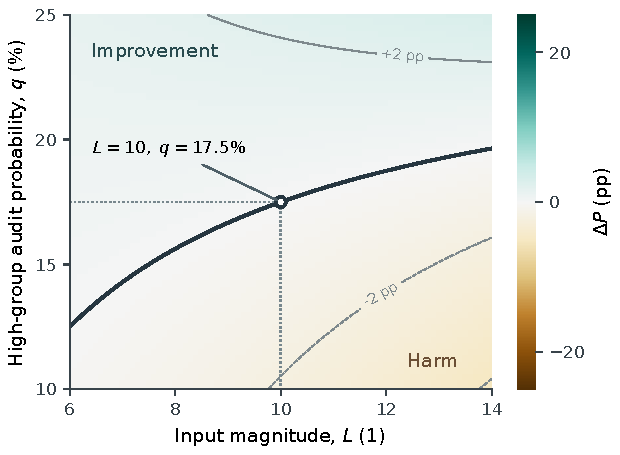
\includegraphics[width=\linewidth]{RSI-audit-figures-20261003/figures/final/audit_detail.pdf}
\end{minipage}\hfill
\begin{minipage}[t]{0.51\linewidth}
\raggedright\textbf{(b)}\par
\centering
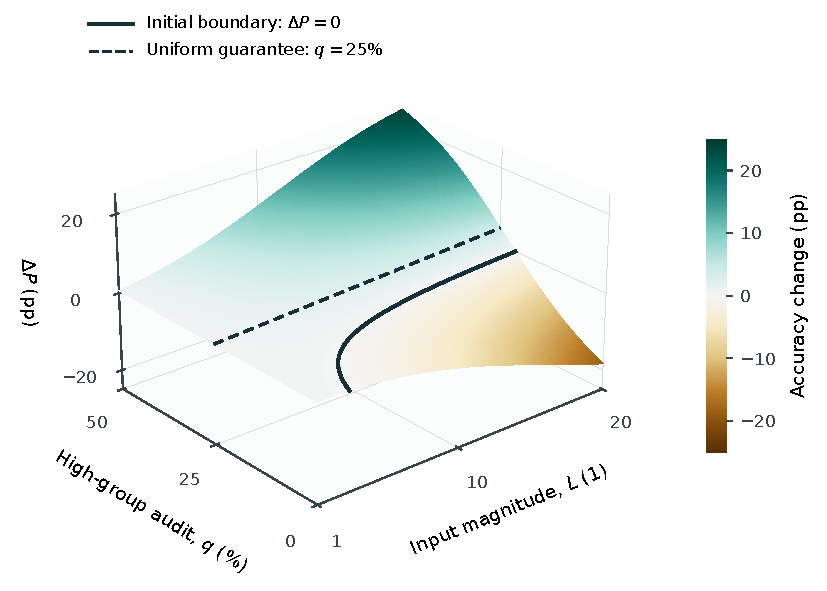
\includegraphics[width=\linewidth]{RSI-audit-figures-20261003/figures/final/audit_surface.pdf}
\end{minipage}
\caption{Supplementary views of the audited initial effect in
Figure~\ref{fig:population-overview}(c,d), with $a=0.75$, $b=0.5$,
$\theta_0=0$, and $\eta=0.1$.
(a) Refined boundary near $(L,q)=(10,0.175)$, using an independent refined grid.
(b) The same initial-effect response surface.
Both show $100[P(-\eta g_{S,q}(0))-1/2]$ in percentage points and retain
the $[-25,25]$ pp color scale. These are deterministic one-step
population calculations, not audited trajectories or language-model results.}
\label{fig:audit-supplement}
\end{figure}


\section{Implementation and Numerical Validation}
\label{app:code}

Table~\ref{tab:code-correspondence} relates the mathematical objects to
their numerical implementation and measurement scope. Implementation
checks establish consistency, not completion of empirical experiments.
No differentiation passes through the verifier.

\begin{table}[H]
\caption{Numerical procedures corresponding to the mathematical statements. Numerical
checks support implementation consistency; the appendix supplies the proofs.}
\label{tab:code-correspondence}
\centering\small
\begin{tabular}{@{}p{0.25\linewidth}p{0.34\linewidth}p{0.35\linewidth}@{}}
\toprule
Mathematical object & Numerical procedure & Interpretation and scope\\
\midrule
Task generators and exact judges
& Procedural task generation and exact correctness evaluation
& Graph distance and exact arithmetic define correctness and target signatures; task specifications are in Appendix~\ref{app:tasks}.\\[3pt]
Logistic acceptance, gradient, and accuracy
& Finite-outcome enumeration of acceptance probabilities and gradients
& Implements the general acceptance rule and gradient in~\eqref{eq:structured-rule} and~\eqref{eq:logistic-gradient}.\\[3pt]
Population trajectories and root checks
& Explicit Euler integration and scalar bisection
& Euler integration and bisection are numerical checks, not the continuous-flow proof or a proof of global uniqueness.\\[3pt]
Matched final subsets
& Joint assignment of prompt roles and common feasible subset sizes
& Common prompts, correct IDs, and quotas support~\eqref{eq:finite-gap}; exact token buckets additionally control graph response lengths.\\[3pt]
Separate arithmetic preparation
& Targeted arithmetic-error selection with response-encoding checks
& Targets \texttt{ignore\_parentheses} and constructs matched response sets; preparation alone performs no optimizer update.\\[3pt]
Shared initialization and one update
& Restoration of a shared adapter and full-batch gradient accumulation
& Per-response loss, accumulation of $g_i/K$ for the unaudited protocol, one clipping operation, and one AdamW step.\\[3pt]
Budgeted auditing after selection
& Budget-constrained correctness queries and reliability weighting
& Integer correctness-query budgets, error removal, optional weights, and pre/post statistics; not the population high-influence policy.\\[3pt]
Audited one-step and iterative training
& Auditing followed by isolated updates or resampled training rounds
& Auditing before training, query records, and durable iterative reuse; completed four-round and unaudited one-step graph results are in Appendix~\ref{app:h100-results}.\\[3pt]
Reference gradient $h$
& Mean canonical-response NLL gradient at the shared initialization
& Unnormalized mean gradient on the canonical-response reference set, in checked shared adapter coordinates. Arithmetic uses bare integer answers, not worked solutions.\\[3pt]
Actual update and projections
& Gradient decomposition and direct parameter-difference measurement
& Records contribution gradients, clipping, parameter displacement, and projections; does not establish a Lipschitz constant $M$.\\
\bottomrule
\end{tabular}
\end{table}

\paragraph{Gradient scaling and reference loss.}
The measured per-response contribution is $g_i/K$ in the unaudited
protocol, whereas $g_i$
in~\eqref{eq:gradient-split} denotes the unscaled response gradient.
Unscaled norms are therefore $K$ times the recorded contribution norms,
while the accumulated contributions already equal the mean gradient.
For audited weighted updates, the recorded contribution is $w_i g_i/W$,
with $W=\sum_iw_i$. Its conversion to an unscaled gradient uses $W/w_i$
for positive-weight responses. Zero-weight responses have no measured gradient
in that update. A normalized reference gradient or a different loss
aggregation is not interchangeable with the unnormalized $h$ defined
in~\eqref{eq:remainder}. The canonical-answer NLL
is a surrogate even when a task admits several correct responses.

\paragraph{Checks and theoretical-policy distinctions.}
Independent numerical checks compare the general logistic implementation
with direct finite-outcome enumeration,
check initial formulas and audit signs, and test finite-pool and smooth-loss
identities on deterministic fixtures. Additional fixtures check the
conditional covariance decomposition, the explicit negative-tail bound,
the accepted-gradient magnitude bound, and equality at the initial audit
contrast threshold. These finite checks are not substitutes for the
universal proofs above. The audit calculation is a
standalone population check: the exact
high-magnitude policy of Theorem~\ref{thm:audit} is not claimed to be
implemented by the language-model auditing pipeline. The finite-budget
policies used in the empirical protocols are specified separately in
Appendix~\ref{app:budgeted-auditing}. Likewise,
scalar-accuracy recursions do not validate these stopped-gradient results.
Specialized parameter settings and the hand-built 128-candidate fixture
are not substitutes for general-parameter proofs. All theoretical
constants are model assumptions, not empirical estimates.

Regression checks verify named-group membership, retained counts and rates,
and initial finite-fixture BCE gradients at $L=1,2,3,10$. Independent
enumeration also verifies this fixture. These checks establish numerical
consistency, not the empirical outcomes in Appendix~\ref{app:h100-results}
or the universal theorems.

\section{Matching Protocol and Certificates}
\label{app:matching}

Each candidate carries a prompt identifier, response identifier, correctness
label, error signature, and supervised token count verified against the
trainer's mask. Let $J_C$ contain prompts with a correct response and $J_E$
contain prompts with an error bucket containing both target and other
signatures. Graph buckets have exact supervised length; arithmetic has no
length tolerance, so its bucket contains all errors on the prompt.
Membership in $J_E$ does not require a correct response.
The joint construction assigns correct roles from $J_C\setminus J_E$ first,
then from flexible prompts, and error roles from the remaining $J_E$.
The roles are exclusive and satisfy both quotas. Correct-role prompts use
the same response ID in both branches;
each error-role prompt contributes one selected response per branch.

\paragraph{Candidate pools, not reference-answer training sets.}
Candidate responses are sampled from the frozen starting model on the
training split, once per seed block before either arm is updated. If the
split contains $M$ prompts and the configuration requests $n$ responses per
prompt, the complete pool contains $Mn$ candidate rows. In the four-round
experiments, $M=2{,}048$ and $n=8$, giving $16{,}384$ responses per block.
Graphs, arithmetic, and different seed blocks have separate pools; within a
block, both arms use the same round-one pool.
The matched $K$ rows are one response for each of $K$ distinct retained
prompts, not $K$ responses per prompt or the whole candidate pool.

Qwen3 models use their chat template with thinking mode disabled.
The four-round studies use temperature $1.3$ and top-$p=1.0$ for
Qwen3-1.7B, and temperature $0.6$ and top-$p=0.9$ for Llama-3.2.
Top-$k$ is disabled, with limits of 2,048 new tokens and 4,096 total tokens;
the recorded repetition-stop rule uses span 128 and maximum period 32.
The one-step graph comparisons reuse each study's actual round-one pools
and shared adapter rather than regenerating nominally equivalent inputs.
Imported Qwen3-4B pools are separate inputs whose original metadata are
preserved; the current repetition-stop setting is not retroactively assigned
to them (Appendix~\ref{app:evaluation}). Pilot pools use development
prompts; main pools use training prompts. Calibration,
reference, and evaluation prompts cannot substitute for training pools.
Arithmetic preparation verifies full $Mn$ coverage. Neither
the exact reference answer nor a correctness label becomes a replacement
training target; directly training on reference answers would be a separate
supervised baseline, not this noisy-verifier intervention.

\paragraph{Truncation and rate denominators.}
The raw pool retains all generated responses, including those marked
\texttt{truncated}. Matching excludes these marked responses before selection.
In~\eqref{eq:finite-rates}, $N^+$ and $N^-$ count correct and incorrect
responses in the entire nontruncated original pool, not only feasible
matching buckets or retained prompt roles. TPR, FPR, and yield therefore
condition on nontruncation; they are not end-to-end acceptance rates over
the raw generated pool. Cut counts are reported separately in
Table~\ref{tab:matching}. This selection convention does not filter
held-out evaluation responses (Appendix~\ref{app:h100-results}).
The separately recorded one-step validation rates use the raw pool.
Those rates differ from the nontruncation-conditional quantities reported
here whenever truncated responses are present.

\paragraph{Explicit per-arm counts.}
The quotas are $C=3K/4$ and $E=K/4$. Table~\ref{tab:subset-counts} makes the
declared ladder explicit for either task family. At $K=64$, both arms use
the same 48 correct prompt--response pairs and the same 16 error-role
prompts, but can retain different responses on those error prompts.
$S$ uses 16 \texttt{nonshortest} graph errors or 16
\texttt{ignore\_parentheses} arithmetic errors. $R$ samples uniformly
within the eligible graph length bucket or, for arithmetic, all errors on
the retained prompt, including target errors; it is not
forced to select 16 non-target errors or to differ from $S$ on every prompt.
The shared correct examples are selected once, not resampled independently
for the two arms. These are protocol counts conditional on feasibility.

\begin{table}[H]
\caption{Declared matching quotas per arm, not empirical measurements.
The comparison requires a common $K$ feasible across every block within a task family.}
\label{tab:subset-counts}
\centering
\begin{tabular}{@{}rrrrr@{}}
\toprule
Common $K$ & Correct $C$ & Incorrect $E$ & Distinct prompts & Precision\\
\midrule
64 & 48 & 16 & 64 & $3/4$\\
32 & 24 & 8 & 32 & $3/4$\\
16 & 12 & 4 & 16 & $3/4$\\
\bottomrule
\end{tabular}
\end{table}

At $K=64$, Equation~\eqref{eq:finite-rates} gives TPR $=48/N^+$ and
FPR $=16/N^-$, whereas precision is $48/64=75\%$. For illustration only,
an original pool with 1,000 correct responses would give TPR $=4.8\%$,
not $75\%$. No such pool count is reported as a measurement.
Matching certificates establish TPR/FPR equality, subset precision, and
identity of the selected correct responses within each block.

Feasibility certificates identify the attempted common sizes for each
block. Training is conditional on a size feasible for all blocks.
An interrupted or unsuccessful search is distinguished from
demonstrated infeasibility. The joint construction never uses gradients or evaluation
outcomes to select candidates. Coincident $R/S$ selections remain in the
record. Algorithm~\ref{alg:matched} summarizes the execution order.

\paragraph{Scope after learning diverges.}
The equal rates and common correct IDs describe the frozen shared-pool
selection. They remain properties of those fixed datasets if more optimizer
steps are taken, but do not imply equal post-update model accuracy.
Fresh pools generated by diverged models can have different $N^+$ and
$N^-$ and different correct responses. Equal retained counts alone then
guarantee neither equal TPR/FPR nor identical correct examples.
The iterative design uses joint matching in round one, followed by
separate per-arm selection. Later rounds
preserve the nominal $K$ and $C:E=3:1$ quotas before auditing, not common
response IDs, selected prompts, token lengths, or numerical TPR/FPR across
different pool denominators. An infeasible arm stops without quota relaxation.
Auditing can change even those retained counts. By contrast,
Theorem~\ref{thm:flow} maintains population TPR/FPR by its explicit
adaptive acceptance rule; the empirical protocol does not supply this guarantee.

One block is one seed-based paired comparison, not a minibatch,
self-training round, or independent model initialization. The one-step
blocks are \texttt{b00}--\texttt{b04}, with pool seeds 0--4 and recorded
generation seeds, reusing the corresponding study's starting inputs.
At $K=64$, five blocks provide five paired comparisons and ten updated
arms, not 64 independent experimental repeats per arm. All $K$ response
gradients accumulate into one AdamW update for $R$ and one for $S$; the
null takes zero updates. Responses are not regenerated inside gradient
computation. The base weights stay frozen, only LoRA parameters change,
and each arm restores the common starting adapter and optimizer state.
The null may perform diagnostic forward/backward passes on $R$'s rows,
but its parameter displacement and projection are zero by construction.

\section{Update Configuration and Numerical Verification}
\label{app:update}

The chosen LoRA configuration is rank $8$, $\alpha=16$, targets
\texttt{q\_proj}/\texttt{v\_proj}, dropout $0$, and bias \texttt{none}.
The selected alpha extends the rank/module/dropout protocol by retaining the
legacy scalar multiplier $\alpha/r=2$. This does not imply equal capacity,
parameter coordinates, gradient norms, or optimizer dynamics across ranks.
The trainable parameter coordinates, dropout state, learning rate,
optimizer settings, clipping threshold, and numerical precision distinguish
the isolated one-step design from the iterative settings in
Appendix~\ref{app:h100-results}.
The executed unaudited one-step graph configuration uses learning rate
$5\times10^{-5}$ and clipping threshold $1.0$, with a dedicated reference
gradient computed at the shared initial adapter and bound to that configuration.
The multiround reference gradient is not substituted for this dedicated gradient.

Microbatch accumulation uses the common denominator $K$ in
Equation~\eqref{eq:response-loss}, rather than a token-weighted average over
responses. The diagnostic records distinguish pre-clipping gradients from
the gradients passed to the optimizer; parameter snapshots are compared in
at least FP32. Per-example norms and split sums are accumulated without
materializing an example-by-parameter matrix.

Gradient composition is checked as a vector identity, not by comparing
norms. Deterministic numerical fixtures use relative tolerance $10^{-4}$
and absolute tolerance $10^{-6}$. The experiment-level criterion is relative $L_2$ error
below $1\%$, together with absolute residuals; a failed check leaves the
diagnostic unvalidated. The completed one-step graph runs have recorded
composition checks, summarized in Section~\ref{app:one-step-results};
the accompanying records do not contain their gradient tensors.

\section{Graph and Arithmetic Task Specifications}
\label{app:tasks}

We describe the procedural task distributions and exact correctness
judges. Settings for the completed studies are reported in
Appendix~\ref{app:h100-results}.

\subsection{Graph shortest paths}
An instance is a connected undirected, unweighted graph $\mathcal G=(V,E)$
and distinct source and target nodes $u,v$. The prompt lists nodes and
edges explicitly. A candidate must parse as a nonempty JSON list of strings
$w=(w_0,\ldots,w_m)$. Define correctness by
\[
 c_{\mathrm{graph}}(\mathcal G,u,v,w)
 =\mathbf1\{w_0=u,\ w_m=v,\ (w_{i-1},w_i)\in E\text{ for all }i,
                    \ m=d_{\mathcal G}(u,v)\},
\]
with malformed outputs assigned correctness zero.
Shortest-path distance is computed by breadth-first search.
Every shortest route is accepted, even if it differs from the particular
route used as the canonical reference response for NLL. The judge does not
require a simple route before checking length: an endpoint-correct,
edge-valid walk with repetitions belongs to \texttt{nonshortest} when
its hop count exceeds the shortest distance.

The generator cycles the declared stratum $d\in\{0,1,2\}$. For ID instances,
$n$ is sampled uniformly from the integers $6+d,\ldots,10+d$. A shuffled
node ordering and a random tree guarantee connectivity. Each unordered
pair is then independently proposed as an additional edge with probability
$p_d\in\{0.35,0.18,0.08\}$; set union removes duplicate edges. Node names
are sampled without replacement from \texttt{v0},\ldots,\texttt{v999}, edge
order is shuffled, and two distinct endpoints are sampled. Thus $d$ is a
generator stratum, not a demonstrated difficulty ordering for the model.
For OOD, $n$ is uniform on $14,\ldots,18$, the backbone is a ring rather
than a random tree, and additional-edge probabilities are $p_d/2$.

The error taxonomy follows the judge's check order: \texttt{format} for
unparseable or ill-typed lists; \texttt{endpoint} for wrong endpoints;
\texttt{nonedge} for an invalid hop; and \texttt{nonshortest} for an otherwise
valid route of incorrect length. This order makes the labels mutually
exclusive. As a judge illustration, on edges
$\{(a,b),(b,d),(a,c),(c,d)\}$ with endpoints $a,d$, both $[a,b,d]$ and
$[a,c,d]$ are correct; $[a,b,a,c,d]$ is \texttt{nonshortest}, and $[a,d]$
is \texttt{nonedge}. These are explanatory examples, not injected training
responses.

\subsection{Exact arithmetic}
The generator samples signed integer leaves uniformly from $[-30,30]$.
For ID stratum $d$, it starts with $3+2d$ leaves and repeatedly combines
two adjacent subexpressions with a uniformly chosen operator in
$\{+,-,\times\}$, enclosing every combination in parentheses. OOD uses
$7+2d$ leaves and negates the complete expression. The current generator
therefore produces integer-valued expressions; it does not implement an
independent held-out-template split.

The arithmetic judge evaluates a bounded abstract syntax tree using
exact rational arithmetic, not floating-point comparison or execution of
candidate code. Its permitted evaluator syntax additionally includes unary
signs and division, although the current generator does not sample division.
The prompt requests a worked solution ending in \texttt{Answer: N}.
The judge reads the final nonempty line, accepting an optional
\texttt{Answer:} prefix and a signed integer or fraction with an unsigned
integer denominator. The numerator and denominator each have at most 128
digits; this is not a 128-character limit on the complete reasoning response.
Invalid syntax or a zero denominator is \texttt{format}. Numerically
equivalent fractions are correct; matching a canonical string is not required.
By contrast, the canonical reference response contains only the bare integer value
for the diagnostic reference NLL. In the saved Llama arithmetic reference
sets, these answers have 2--4 supervised tokens (median 3). The projection
can therefore reflect response-format changes as well as mathematical
content; its sign is not evidence of arithmetic correctness degradation or
directly comparable to a graph projection. The format mismatch alone does
not establish the cause of the observed positive arithmetic projections.

Let $V(e)$ be the exact expression value and let $e_{\setminus()}$ be the
expression obtained by deleting all parentheses. After excluding correct
responses, the target signature is
\[
 \texttt{ignore\_parentheses}
 \quad\Longleftrightarrow\quad
 V(e_{\setminus()})\text{ exists},\quad
 V(e_{\setminus()})\ne V(e),\quad \hat y=V(e_{\setminus()}).
\]
If this test fails, a wrong answer equal to $-V(e)$ receives \texttt{sign};
remaining parseable errors receive \texttt{other}. Parenthesis errors take
precedence over sign errors when both descriptions apply. For example,
$(2+3)\times4$ has correct value $20$, deletion-of-parentheses value $14$,
sign error $-20$, and other error $21$. For $(2+3)$ the deletion value is
also $5$, so response $5$ is correct, not a target error. These examples
describe the judge; the empirical pools instead contain saved model responses.

\subsection{Task-specific matched intervention and empirical scope}
Graph selection targets \texttt{nonshortest} errors, while arithmetic
selection targets \texttt{ignore\_parentheses} errors. For each
task family separately, an error-role prompt must have a bucket containing
both target and non-target errors: an exact-length bucket for graphs, or
all errors on the prompt for arithmetic, without length matching.
$R$ samples uniformly from that bucket, while $S$ samples target errors.
Coincidences are retained. Common correct-response IDs, prompts, graph
per-prompt token counts,
$C:E=3:1$, unit weights, and the shared $64\to32\to16$ ladder are checked
before training. Missing target errors do not trigger a replacement
signature, manufactured responses, seed changes, or a tolerance other than
the one configured for the task. Arithmetic's no-tolerance setting was
specified before the experiments; length is not controlled in that extension.
The constraints are not imposed between a graph pool and an arithmetic pool.

Arithmetic preparation verifies complete candidate coverage and block-local
selection from the original pools. Supervised token counts are recomputed
from the response-only training encoding, including the end-of-sequence
token; generation counts are not substituted and overlong examples are
excluded rather than truncated. The matched datasets retain the original
prompt--response pairs with unit weights. Correctness labels, error
signatures, and replacement oracle answers are not training targets.

\paragraph{Dataset defaults versus executed settings.}
The dataset generator defaults to 2,048 prompts per training split,
512 development prompts, 500 calibration prompts, 64 gradient-reference
prompts, 2,000 ID evaluation prompts, and 1,000 OOD evaluation prompts.
These are generator defaults, not verified sizes of a supplied run.
Fresh training splits supply candidate prompts for successive rounds;
they do not create additional independent replicates. Checks for duplicate content verify split
isolation. Arithmetic and graph risk readouts remain
separate, and the reference split is used only for diagnostics. Content-level
isolation does not itself ensure disjoint expression templates or graph
isomorphism classes. The OOD generators jointly change size and structure;
they are not factorial ablations isolating each shift component.

\section{Evaluation Design and Extensions}
\label{app:evaluation}

The one-step design comprises graph comparisons with Qwen3-1.7B,
Qwen3-4B, and Llama-3.2-3B, and planned arithmetic comparisons with
Llama-3.2-1B/3B. Each uses five paired blocks and unaudited $R/S$/null
arms. The graph results appear in Table~\ref{tab:one-step-heldout}.
Response-generation settings are model-specific.
Training, development, calibration, gradient-reference, ID evaluation, and
OOD evaluation splits are mutually exclusive. Cross-split content comparisons check
duplication; identifiers do not encode split names. The reference split has
64 prompts and is used only for diagnostics. In this design, reference and
test sets are excluded from construction, matching, and tuning; final-test
decoding occurs after the updates. Task distributions, split sizes,
generation parameters, and decoding are specified independently of test outcomes.

The one-step evaluation uses one greedy answer on each of the 2,000 ID and
1,000 OOD questions under a common decoding protocol. The shared initial
model supplies one null baseline per combination; the ten updated checkpoints
are evaluated separately, giving eleven checkpoints, not fifteen independent
models. Repeated displays of the baseline add no replicates. ID and OOD
are analyzed separately. Block-level
readouts combine task risk, parameter change, reference-loss projection,
response length, and accepted-error signatures. Coincident selections and
zero or negative effects remain part of the comparison.
For block $j$, define
\begin{equation}
 \begin{aligned}
 \Delta\widehat{\mathcal R}_{j,v}
 &=\widehat{\mathcal R}_{j,v}-\widehat{\mathcal R}_{j,0},\\
 D_j&=\Delta\widehat{\mathcal R}_{j,S}
       -\Delta\widehat{\mathcal R}_{j,R}.
 \end{aligned}
 \label{eq:risk-readout}
\end{equation}
Intervals conditional on these adapters do not quantify variation across
arbitrary model initializations. The primary contrast is $S-R$ in
ID greedy Pass@1, equal to $-D_j$ in~\eqref{eq:risk-readout}; positive values
favor $S$. Pointwise paired Student-$t$ intervals over the five blocks have
four degrees of freedom. OOD and diagnostics are separate readouts. Five
pairs do not support multi-covariate regression or broad predictive claims.
All scheduled blocks and zero-effect outcomes remain in the analysis;
responses and rounds are not additional replicates. This revised plan is
not evidence of pre-outcome registration of the four-round study.

The completed Qwen3-4B graph comparison uses imported round-one pools and the
associated shared adapter and matching record. These inputs predate the
repetition-stop rule.
Their generation metadata remain unchanged; greedy evaluation uses its own
recorded stopping settings. This difference in pool generation remains relevant
to the completed one-step comparison (Section~\ref{app:one-step-results}).

Sensitivity to a small number of additional updates on the same fixed pool
is distinct from resampled iterative self-training and has not been evaluated.
Correctness auditing is implemented for one-step and iterative protocols
under equal per-arm-round query budgets, with separate query and
cost records (Appendix~\ref{app:budgeted-auditing}). A mismatched-subset
control would isolate the effect of relaxing a particular constraint;
no such comparison is reported.

\paragraph{Replication and statistical power.}
Larger paired-seed studies could improve precision, with sample sizes
motivated by development-set variability and a prespecified meaningful
effect. The present design offers no general power guarantee. The common
$K$ constraint applies to every scheduled block within a task family, so
feasibility-based exclusion would change the target comparison. Retained
examples are training observations, not independent model-level replications.

\paragraph{Implemented resampled trajectories.}
The iterative design specifies four rounds, separate from
the complementary one-step comparison. Round one uses the shared matched pool;
later rounds generate fresh responses from each arm's previous checkpoint
on a common fresh prompt set. Defaults request 512 later-round prompts and
four responses per prompt. Each arm independently selects $K$ rows with
$C:E=3:1$ before auditing; quota failure stops that arm. These constraints
do not match actual TPR/FPR across different original-pool denominators,
nor selected prompts, correct IDs, or token lengths. The supplied configuration
uses one epoch and effective batch size four, giving 16 optimizer updates
per unaudited $K=64$ round. Auditing can reduce this count
(Appendix~\ref{app:budgeted-auditing}); a round is not one optimizer step.
Fresh optimizer state is used each round, while adapter parameters continue
from the preceding round. The reference gradient remains evaluated at the
common initial adapter, not recomputed at each current checkpoint.
The completed four-round graph endpoints appear in
Table~\ref{tab:audit-results}, separately from the isolated one-step
comparison in Table~\ref{tab:one-step-heldout}. All intermediate rounds are retained in
Appendix~\ref{app:h100-results}, rather than selecting a best round on
the final test set. The completed studies use larger candidate pools than
the later-round defaults above; their generation settings and measured
update counts are documented there. The Llama and Qwen3-1.7B trajectories
also extend to eight rounds; four rounds remain the primary horizon,
with round-eight contrasts reported in Appendix~\ref{app:qwen-four-round}.
Rotating verifier blind spots
remains an extension. Distinguishing error identity from its timing would be necessary
to identify a persistence effect, which the one-step comparison does not test.

\paragraph{Optional learned-verifier validation.}
The primary $R/S$ intervention is controlled simulated acceptance, with
exact programmatic judges supplying correctness labels. A frozen same-model
verifier, an evolving solver acting as its own verifier, or a frozen
different-family verifier would require a separate protocol: no reference
answer in verifier input, threshold calibration on a disjoint calibration
split, and measured operating rates on each candidate distribution.
These comparisons also change verifier competence and cannot replace the
matched-subset control. No learned-verifier outcome or finite-sample
audit-complexity guarantee is reported. The completed resampled
multi-round graph results are in Appendix~\ref{app:h100-results}.

\section{Computing Resources and Cost Accounting}
\label{app:cost}

The Llama and Qwen3-1.7B four-round graph experiments used one NVIDIA H100 80\,GB GPU per
job. For the Llama comparison, shared pool generation took 1 h 45 min
28 s, unaudited training and evaluation took 7 h 12 min 42 s, and audited
training and evaluation took 7 h 16 min 6 s. These three distinct jobs
total 16.24 allocated GPU-hours. This is a \emph{partial job subtotal},
not the full study cost or isolated optimizer time: it excludes other
experiments, data preparation, and unreported attempts.

The isolated Qwen3-1.7B study used an NVIDIA RTX 4070 laptop GPU with
8\,GB memory on Windows. The Qwen3-4B and Llama one-step studies used
NVIDIA A100-SXM4 GPUs with 40\,GB memory through Colab. Model execution
used PyTorch~\citep{paszke2019pytorch}, Transformers~\citep{wolf2020transformers},
and PEFT~\citep{peft}; the underlying runtimes differed
across platforms. Each one-step comparison therefore uses its own null
baseline, and bitwise cross-platform reproducibility is not claimed.

The Qwen3-4B audited four-round study used two NVIDIA A100-SXM4 GPUs
with 80\,GB memory, with independent workers for the $R/S$ arms.
The Qwen3-4B unaudited four-round study used one NVIDIA GeForce
RTX 5090 GPU on Windows.

\paragraph{Model and software licenses.}
Qwen3-1.7B and Qwen3-4B are distributed under the Apache License 2.0;
Llama-3.2-1B/3B-Instruct use the Llama 3.2 Community License Agreement.
PyTorch uses a BSD-style license, while Transformers and PEFT use the
Apache License 2.0. The task datasets are generated procedurally.

\section{Finite-Budget Auditing}
\label{app:budgeted-auditing}

We specify the finite-budget correctness-auditing intervention.
The primary matched-rate isolation study remains unaudited. The extension
spends additional correctness queries after selection and before training;
it is not a learned verifier, a replacement-answer intervention, or an
implementation of Theorem~\ref{thm:audit}'s known-magnitude policy.
The completed four-round Llama graph pair is reported below and in
Appendix~\ref{app:h100-results}. The Qwen four-round graph pairs
and three unaudited one-step graph comparisons are reported in
Sections~\ref{app:qwen-four-round}, \ref{app:qwen4b-four-round},
and~\ref{app:one-step-results}.

\subsection{Budget, information access, and allocation}

Let $D_{j,v,t}$ be the pre-audit selected subset for block $j$, arm $v$,
and round $t$, with $K_{j,v,t}$ rows. An active audit policy receives an
integer budget $B_{\mathrm{qry}}\geq0$ and makes
\[
 b_{j,v,t}=\min(B_{\mathrm{qry}},K_{j,v,t})
\]
correctness queries, sampling without replacement. With policy
\texttt{none} and budget zero, auditing is a zero-query identity.
Both queried correct and queried incorrect candidates consume budget.
The allocator receives candidate IDs, task IDs, responses, and weights;
task metadata supplies the generator difficulty stratum.
Current correctness and error-taxonomy fields
are stripped before allocation. Only subsequent exact checker calls reveal
the queried correctness bits. The graph checker uses shortest-path distance;
the arithmetic checker uses exact expression evaluation. Canonical answers
are not revealed to the allocator or substituted as training targets.

\paragraph{Uniform.}
The uniform policy samples $b_{j,v,t}$ candidates from the full selected subset, giving each
candidate inclusion probability $b_{j,v,t}/K_{j,v,t}$ when $K_{j,v,t}>0$.

\paragraph{Balanced and adaptive.}
Balanced and adaptive policies partition the selected rows into nonempty
strata $g$ with sizes $n_g$. Each stratum receives one query when the budget permits; if there are fewer
queries than strata, the implementation seeds the first strata in sorted
order. Remaining queries are allocated successively to an uncapped stratum
maximizing $\lambda_g/(m_g+1)$, with deterministic tie resolution, where
$m_g$ is its allocated count. Balanced allocation uses $\lambda_g=1$.
Adaptive allocation uses
\[
 \lambda_g=n_g\,
 \operatorname{Quantile}_{0.9}
 \bigl(\operatorname{Beta}(1+e_{g,t-1},1+c_{g,t-1})\bigr),
\]
with the same arm's immediately preceding audit counts of errors and
correct responses, defaulting to zero when unavailable. This is a
history-based allocation heuristic, not an optimal influence estimator.
It does not accumulate all past rounds or use the other arm's history.
Conditional on the allocation, candidates are sampled uniformly within each stratum;
queried candidates have inclusion probability $m_g/n_g$.
Allocation is fixed before any current-round query label is observed.
Paired arms share the block's audit RNG seed, but distinct responses and
arm-specific histories can yield different queried IDs and allocations.
In a one-step run, adaptive allocation has no previous-round observations.

\subsection{Retention, weights, and optimizer semantics}

Queried errors are removed, while queried correct responses retain weight one.
Without reliability weighting, all unaudited responses retain weight one.
With weighting enabled and $m_g=e_g+c_g>0$ current-round queries in stratum
$g$, an unaudited response receives
\[
 w_g=\max\left\{0,1-2\frac{1+e_g}{2+m_g}\right\}.
\]
An unqueried stratum retains weight one. The fraction
$(1+e_g)/(2+m_g)$ is the Beta$(1,1)$ posterior mean error probability;
the clipped transformation is a reliability heuristic, not inverse-propensity
weighting or an unbiased gradient correction. Zero-weight rows remain in
the retention record but contribute nothing to optimization.

An audited one-step update accumulates $w_i g_i/W$ for all positive-weight rows,
where $W=\sum_iw_i$, clips once, and takes one AdamW update if $W>0$.
If $W=0$, it takes zero updates and saves an unchanged adapter. The frozen
null remains unaudited and takes no optimizer update.
Audited one-step updates are an implemented extension; the reported
isolated one-step comparisons use the strict unaudited protocol.

Iterative training continues each arm from its preceding adapter and
starts a fresh optimizer each round. It normalizes weights within each
effective batch, rather than using one denominator for the entire round.
For $n^+_{j,v,t}$ positive-weight rows, effective batch size $m$, and
$E_{\mathrm{ep}}$ epochs, the expected actual step count is
\[
 U_{j,v,t}=E_{\mathrm{ep}}\left\lceil n^+_{j,v,t}/m\right\rceil.
\]
Observed step counts are checked against this expression. With no
positive-weight examples, the adapter remains unchanged. The four-round
design uses one epoch,
effective batch size four, and microbatch size two: an unaudited feasible
$K=64$ round takes 16 steps, consistent with the completed graph records.
Filtering and weighting can reduce the count. Equal audit budgets therefore
do not imply equal retained training volume or equal optimizer work.

The common-pool construction and its $48/16$, $24/8$, or $12/4$ quotas
are certified before auditing. Post-audit correct IDs, prompt coverage,
lengths, counts, weights, rates, and correct-gradient contributions need
not agree. Pre/post statistics therefore describe different training sets,
and~\eqref{eq:finite-gap} is not a post-audit cancellation identity.
In iterative rounds two and later,
the pre-audit pools already differ across arms: independent quota matching
does not imply equal numerical TPR/FPR or common responses.

\subsection{Experimental settings and query accounting}

The reported audited multiround experiments use $B_{\mathrm{qry}}=16$, adaptive
allocation, and reliability weighting; corresponding unaudited runs are
controls. Each reported round samples eight responses for 2,048 prompts.
The generation settings and measured update counts are documented in
Appendix~\ref{app:h100-results}; they differ from the smaller
later-round defaults. The primary one-step comparison is unaudited.
Audited one-step comparisons, other budgets, and other policies remain
extensions rather than completed experiments.

For each audited arm-round, the recorded statistics include requested and actual
query counts, candidate IDs, correctness-only labels, inclusion probabilities,
per-stratum audit counts, and before/after statistics. Training uses
only prompt--response pairs and weights, not correctness
or error-taxonomy labels. Experimental truth labels remain available
internally for the one-step correct/error gradient diagnostic; this is
measurement access, not an input to audit allocation or to the SFT loss.
Actual and cumulative queries and optimizer steps are recorded separately.

Pre/post TPR and FPR use the same nontruncated original candidate pool's
$N^+$ and $N^-$,
not the retained subset as denominator. The audit statistics comprise
retained $K,C,E$, precision, yield, positive-weight correct/error counts
and rates, weight sum $W$, and effective sample size
\[
 \operatorname{ESS}=\frac{W^2}{\sum_iw_i^2},
\]
with ESS zero when the weight sum is zero. A retained row and a
positive-weight training example are not the same accounting unit.
Undefined rates for empty denominators remain unavailable, not zero.

For a completed block with two arms and $T$ feasible selected rounds each,
the additional intervention-query count is at most
$2T\min(B_{\mathrm{qry}},K)$ when the pre-audit size is the common $K$.
Infeasible rounds stop before querying. At $B_{\mathrm{qry}}=16$, $K=64$,
and $T=4$, the design cap is 128 queries per completed block across the arm
pair, i.e., 64 per arm. The completed graph study reaches this per-arm cap;
the expression is a design bound for other runs.
At $B_{\mathrm{qry}}\geq K$, all selected examples are queried: this is
full trusted filtering, not a scarce-budget condition. The requested
budget's effective fraction depends on the realized $K$;
budget 16 is a quarter at $K=64$ but a full audit at $K=16$.

The reported query count includes only additional online intervention queries.
It excludes exact labels used to construct the controlled selections,
match/diagnose pools, build reference responses, or judge evaluation outputs.
It is therefore not the total trusted-label cost of the study, and the
current comparison does not establish end-to-end trusted-label savings.
Query accounting also differs from the
population initialization fraction $B(q)$ in Corollary~\ref{cor:audit-budget}.

Completed iterative audit batches remain in the query accounting even
when training is interrupted, and their labels are reused if training
resumes. An interruption before an audit batch is fully recorded can
repeat local checker calls; the accounting therefore does not establish
an exactly-once guarantee for a paid external oracle. Audited and
unaudited conditions are distinct interventions, not retrospective
reinterpretations of the same training run.

\subsection{Independent evaluation and empirical scope}

Corresponding conditions share the starting adapter and round-one pools.
The reference gradient is computed at this initialization under the
specified training configuration. This calculation uses
only the disjoint gradient-reference split, with uniform reference weights
and no audit queries. It does not audit the diagnostic reference set.

Checkpoint ID/OOD evaluation is separate from training and uses the
common greedy protocol. Protocol-consistency checks verify evaluation
coverage independently of training completion; completed training alone
does not establish complete held-out evaluation.
The strict unaudited matching certificate does not certify an
audited training subset; that analysis relies on the pre/post audit records.
Risk changes are relative to the common base and the corresponding
unaudited arm, with tasks, policies, budgets, and rounds kept distinct.
The accompanying readouts include block-level outcomes, cumulative queries,
post-audit composition, positive-weight coverage, ESS, optimizer steps, and
independent ID/OOD risk. For iterative displacement projections, $h$ stays at the common
initialization; it is not a freshly evaluated local gradient at each round.
A favorable projection alone does not establish held-out task improvement.

Table~\ref{tab:audit-results} in Section~\ref{sec:audit-results} reports
the completed four-round Llama graph endpoint and paired audit changes.
The separate one-step graph endpoints appear in Table~\ref{tab:one-step-heldout}.
Table~\ref{tab:audit-composition} gives completed graph composition and
actual cumulative steps/queries; this is not a completed budget sweep.
Appendix~\ref{app:h100-results} documents the greedy protocol, five-block descriptive
intervals, and coverage of every incomplete run. These settings differ
from the smaller candidate-pool defaults.
Earlier checkpoints and deterministic fixtures are not substituted
for unavailable round-four outcomes. The available records do not
establish a preregistered confirmatory analysis or prompt-bootstrap intervals.

\begin{table}[H]
\caption{Round-four composition and cumulative effort for Llama-3.2-3B graph. Individually listed rows use adaptive auditing, $B_{\rm qry}=16$; the first row is the unaudited reference for either arm in every block. The $K'/n^+$ column gives the retained and positive-weight response counts, respectively; $C/E$ gives retained correct/error counts. Composition describes the final round, whereas Steps/$Q$ are cumulative over four rounds. ESS is reported in the audit summaries and cannot be independently reconstructed because raw weight vectors are unavailable.}
\label{tab:audit-composition}
\centering\small\setlength{\tabcolsep}{6pt}
\begin{tabular}{@{}llccccc@{}}
\toprule
Block/policy & Arm & $K'/n^+$ & $C/E$ & ESS & Steps & $Q$\\
\midrule
All blocks, none & R/S & 64/64 & 48/16 & 64.00 & 64 & 0\\
\midrule
b00 & R & 63/63 & 48/15 & 58.69 & 53 & 64\\
b00 & S & 60/45 & 48/12 & 36.37 & 53 & 64\\
b01 & R & 60/60 & 48/12 & 45.32 & 57 & 64\\
b01 & S & 60/60 & 48/12 & 43.80 & 59 & 64\\
b02 & R & 63/63 & 48/15 & 59.76 & 50 & 64\\
b02 & S & 59/47 & 48/11 & 36.70 & 56 & 64\\
b03 & R & 61/39 & 48/13 & 37.86 & 57 & 64\\
b03 & S & 61/61 & 48/13 & 46.15 & 63 & 64\\
b04 & R & 61/61 & 48/13 & 45.15 & 54 & 64\\
b04 & S & 61/61 & 48/13 & 50.25 & 44 & 64\\
\bottomrule
\end{tabular}
\end{table}


Regression checks cover query caps,
hidden-label isolation, deletion/weighting, original-pool denominators,
zero-signal updates, and reuse of completed audit batches. Integration
fixtures replace model generation and training with controlled stand-ins;
separate toy-LoRA fixtures exercise the weighted one-step optimizer.
These checks establish neither empirical auditing benefits nor a
finite-sample query-complexity theorem.

\raggedbottom
\section{Full Empirical Results and Validation}
\label{app:h100-results}

\subsection{Experiment coverage}
Table~\ref{tab:h100-progress} summarizes the completed graph experiments:
six four-round model--policy comparisons and three unaudited one-step
comparisons, each with five paired blocks and both held-out splits.
The model-specific results follow below. Arithmetic feasibility is assessed
for Llama-3.2-1B/3B.

\begin{table}[H]
\caption{Completed graph experiment matrix. Each row has five paired blocks and $R/S$ arms, evaluated on 2,000 ID and 1,000 OOD questions. Four rounds yield 40 trained checkpoints; one step yields ten. Evaluation counts include one unupdated base/null per split, not independent baseline replications.}
\label{tab:h100-progress}
\centering\small\setlength{\tabcolsep}{4pt}
\begin{tabular}{@{}lllccc@{}}
\toprule
Model & Design & Audit & Paired blocks & Trained checkpoints & Evaluated per split\\
\midrule
Llama-3.2-3B & Four rounds & None & 5 & 40 & 41\\
Llama-3.2-3B & Four rounds & B=16 & 5 & 40 & 41\\
Qwen3-1.7B & Four rounds & None & 5 & 40 & 41\\
Qwen3-1.7B & Four rounds & B=16 & 5 & 40 & 41\\
Qwen3-4B & Four rounds & None & 5 & 40 & 41\\
Qwen3-4B & Four rounds & B=16 & 5 & 40 & 41\\
\addlinespace
Llama-3.2-3B & One step & None & 5 & 10 & 11\\
Qwen3-1.7B & One step & None & 5 & 10 & 11\\
Qwen3-4B & One step & None & 5 & 10 & 11\\
\bottomrule
\end{tabular}
\end{table}


\subsection{Evaluation definitions and uncertainty}
Evaluation uses one greedy answer per held-out question at each checkpoint,
with temperature zero,
top-$p=1$, and the same length and repetition-stop rules across the pair.
The two conditions use identical questions, task datasets, base models,
and decoding settings within each split. ID has 2,000 questions
(667/667/666 by difficulty); OOD has 1,000 (334/333/333).
Pass@1 is the fraction judged correct; task error is its complement.
All generated answers enter these denominators, including truncated answers,
which are judged as generated. The target-error fraction counts \texttt{nonshortest} among \emph{all}
answers, rather than conditioning on incorrect answers.

For a completed arm/round, let $x_j$ be its metric on block $j$.
The descriptive interval is
\[
 \bar x\ \pm\ t_{0.975,4}\frac{s_x}{\sqrt5},\qquad
 s_x^2=\frac14\sum_{j=1}^5(x_j-\bar x)^2,
 \quad t_{0.975,4}=2.776445\ldots.
\]
For $S-R$, the interval uses the five within-block differences.
In Table~\ref{tab:audit-results}, it instead uses
$d_j=\widehat e^{\rm audit}_j-\widehat e^{\rm none}_j$ in the same arm
and split; this differs from the plots' $S-R$ contrast. Both types of
interval are independently recalculated from the checkpoint summaries.
One common base checkpoint is not five independent initial models: no
block-uncertainty interval is estimated for round zero.

These are pointwise, descriptive block-$t$ intervals, conditional on the
fixed question sets. Five blocks give imprecise sampling distributions;
normality of block differences and generalization to a broader model/task
population are not established. No correction is made for the many
round/metric/split/policy comparisons, and no selected nominal $p$-value
is interpreted as confirmatory evidence. An immutable pre-outcome analysis
registration is not documented. Raw evaluated responses are unavailable
for the Llama study and the earlier incomplete series, so question-level
bootstrap intervals and independent rejudging are not claimed for those
conditions. The available Qwen3-4B audited responses are independently
rejudged in Section~\ref{app:qwen4b-four-round}; its reported intervals
nevertheless use the same block-level definition.

Across the three models, the descriptive 95\% intervals include zero for
all four-round endpoint accuracy contrasts (both $S-R$ and same-arm audit
changes), primary one-step ID accuracy contrasts, and paired one-step
reference projections. This does not establish equivalence of the arms
or policies. Target-incidence and secondary OOD contrasts are reported
individually in the following subsections.

\subsection{Llama-3.2-3B: four-round graph replication}
\label{app:llama-four-round}
Both policies comprise five paired blocks and four training rounds.
The Llama-3.2-3B-Instruct conditions share round-one candidate pools,
task datasets, and initial adapter parameters. Each arm resumes its own
previous LoRA checkpoint in later rounds, with fresh AdamW state.
Training uses bfloat16, rank 8, $\alpha=16$, zero dropout,
\texttt{q\_proj}/\texttt{v\_proj}, one epoch, learning rate
$2\times10^{-4}$, zero weight decay, microbatch 2, and effective batch 4.
Each round's 2,048 prompts yield eight responses per prompt at temperature
$0.6$ and top-$p=0.9$, with a 2,048-new-token cap, 4,096-token sequence
limit, and repetition stopping (span 128, maximum period 32).
Pool seeds are 0--4, with separate training and subsequent generation
seeds for each block and round. Later responses come from each arm's
preceding checkpoint and are not jointly rate-matched.
The initial LoRA adapter has zero $B$ matrices, so its predictions coincide
with the untrained base. The separate reference-split gradient $h$ stays
fixed throughout training, rather than being refreshed each round.

\begin{table}[H]
\caption{Round-one pre-audit matching for Llama-3.2-3B graph. Both arms have $K=64$, $C/E=48/16$, precision $0.75$, and unit weights. $N^+/N^-$ count eligible original-pool responses after removing cut answers. Matching certificates confirm shared prompts and correct responses with identical per-prompt supervised-token counts. Target hits count target-type responses among 16 selected errors; uniform selection in $R$ can include these errors. Actual training uses 16 unaudited optimizer steps per round, rather than the certificate's nominal single-update designation.}
\label{tab:matching}
\centering\small\setlength{\tabcolsep}{4pt}
\begin{tabular}{@{}lcccccc@{}}
\toprule
Block & $N^+/N^-$ & Cut & TPR/FPR & Yield & Target hits $R/S$ & Constraints\\
\midrule
b00 & 3848/12389 & 147 & $0.012474/0.001291$ & 0.003942 & 9/16 & pass\\
b01 & 3877/12369 & 138 & $0.012381/0.001294$ & 0.003939 & 9/16 & pass\\
b02 & 3805/12458 & 121 & $0.012615/0.001284$ & 0.003935 & 12/16 & pass\\
b03 & 3810/12421 & 153 & $0.012598/0.001288$ & 0.003943 & 9/16 & pass\\
b04 & 3838/12414 & 132 & $0.012507/0.001289$ & 0.003938 & 13/16 & pass\\
\bottomrule
\end{tabular}
\end{table}

\begin{table}[H]
\caption{Llama-3.2-3B graph endpoints after four rounds. Target rates count nonshortest answers among all evaluated questions. Paired $S-R$ differences are within policy, with descriptive 95\% block-$t$ half-widths over five blocks. The base is one shared checkpoint.}
\label{tab:llama-endpoints}
\centering\small\setlength{\tabcolsep}{3pt}
\begin{tabular}{@{}lllllll@{}}
\toprule
Split & Policy & Base & Pass@1 $R/S$ & $S-R$ Pass@1 & Target $R/S$ & $S-R$ target\\
\midrule
ID & None & 0.2480 & 0.558/0.560 & $0.002\pm0.105$ & 0.146/0.183 & $0.036\pm0.103$\\
ID & B=16 & 0.2480 & 0.586/0.620 & $0.034\pm0.067$ & 0.129/0.137 & $0.007\pm0.063$\\
OOD & None & 0.2090 & 0.430/0.447 & $0.017\pm0.081$ & 0.090/0.118 & $0.029\pm0.084$\\
OOD & B=16 & 0.2090 & 0.449/0.476 & $0.027\pm0.044$ & 0.074/0.120 & $0.046\pm0.091$\\
\bottomrule
\end{tabular}
\end{table}


Table~\ref{tab:h100-rounds} includes every completed round; the base
is displayed once per split. Table~\ref{tab:h100-blocks} retains all
five endpoint blocks. The original unaudited, audited, and joint comparison
plots are included unchanged in
Figures~\ref{fig:llama-raw-unaudited}--\ref{fig:llama-raw-comparison-difficulty},
including both ID/OOD difficulty breakdowns. Their round-zero zero-width
bars are a plotting convention for
the common base, not a precision claim from five independent fits.
Figure~\ref{fig:graph-four-round}(a--b) is a compact vector replot of the same validated
accuracy summaries; no curves were smoothed or observations removed.

The completed study does not exhibit opposite overall learning directions:
both selection arms improve on both splits.
Auditing's mean endpoint accuracy improves, especially ID $S$. However, the
audited OOD $S$ target-error rate is $0.120$, compared with $0.118$
without auditing; target-error suppression is not uniform across splits.
These findings constrain the empirical interpretation of the population
example rather than verifying a universal ordering of verifiers.

Format-error incidence also declines from base $0.014$ ID and $0.023$
OOD. Round-four ID fractions are $0.0007/0.0012$ for unaudited $R/S$
and $0.0015/0.0008$ with auditing; OOD fractions are $0.0022/0.0020$
and $0.0048/0.0034$, respectively. These descriptive means remain in
the supplementary measurements and do not imply an additional significance claim.

\begin{table}[H]
\caption{All completed graph rounds, Llama-3.2-3B. Values are fractions: mean $\pm$ pointwise 95\% Student-$t$ half-width over five blocks. $S-R$ intervals are computed from within-block differences, not differences of independent means. Target is \texttt{nonshortest} incidence among all answers. Each base is one shared checkpoint, not five independently trained models; no uncertainty estimate is supplied for it. No multiplicity adjustment is applied across rounds, splits, metrics, or policies.}
\label{tab:h100-rounds}
\centering\footnotesize\setlength{\tabcolsep}{3pt}
\begin{tabular}{@{}llccccccc@{}}
\toprule
Split & Audit & $t$ & Pass@1 $R$ & Pass@1 $S$ & $S-R$ & Target $R$ & Target $S$ & $S-R$\\
\midrule
ID base & --- & 0 & $0.248$ & $0.248$ & --- & $0.127$ & $0.127$ & ---\\
ID & None & 1 & $0.471\pm0.039$ & $0.482\pm0.038$ & $0.011\pm0.020$ & $0.152\pm0.013$ & $0.170\pm0.018$ & $0.018\pm0.017$\\
ID & None & 2 & $0.499\pm0.049$ & $0.532\pm0.056$ & $0.033\pm0.099$ & $0.150\pm0.023$ & $0.176\pm0.050$ & $0.026\pm0.064$\\
ID & None & 3 & $0.509\pm0.091$ & $0.544\pm0.057$ & $0.034\pm0.100$ & $0.152\pm0.020$ & $0.192\pm0.055$ & $0.040\pm0.067$\\
ID & None & 4 & $0.558\pm0.081$ & $0.560\pm0.068$ & $0.002\pm0.105$ & $0.147\pm0.041$ & $0.183\pm0.069$ & $0.036\pm0.103$\\
ID & B=16 & 1 & $0.452\pm0.023$ & $0.447\pm0.011$ & $-0.006\pm0.015$ & $0.175\pm0.039$ & $0.193\pm0.046$ & $0.018\pm0.021$\\
ID & B=16 & 2 & $0.506\pm0.020$ & $0.531\pm0.066$ & $0.025\pm0.058$ & $0.147\pm0.024$ & $0.152\pm0.063$ & $0.005\pm0.054$\\
ID & B=16 & 3 & $0.548\pm0.050$ & $0.585\pm0.044$ & $0.036\pm0.033$ & $0.155\pm0.055$ & $0.136\pm0.063$ & $-0.019\pm0.063$\\
ID & B=16 & 4 & $0.586\pm0.073$ & $0.620\pm0.031$ & $0.034\pm0.067$ & $0.129\pm0.049$ & $0.137\pm0.068$ & $0.007\pm0.063$\\
\midrule
OOD base & --- & 0 & $0.209$ & $0.209$ & --- & $0.073$ & $0.073$ & ---\\
OOD & None & 1 & $0.372\pm0.028$ & $0.390\pm0.024$ & $0.018\pm0.019$ & $0.070\pm0.009$ & $0.082\pm0.010$ & $0.012\pm0.012$\\
OOD & None & 2 & $0.378\pm0.037$ & $0.424\pm0.042$ & $0.045\pm0.059$ & $0.077\pm0.018$ & $0.102\pm0.048$ & $0.025\pm0.061$\\
OOD & None & 3 & $0.399\pm0.064$ & $0.435\pm0.046$ & $0.037\pm0.070$ & $0.079\pm0.008$ & $0.126\pm0.051$ & $0.047\pm0.054$\\
OOD & None & 4 & $0.430\pm0.070$ & $0.447\pm0.054$ & $0.017\pm0.081$ & $0.090\pm0.040$ & $0.118\pm0.061$ & $0.029\pm0.084$\\
OOD & B=16 & 1 & $0.366\pm0.019$ & $0.370\pm0.011$ & $0.004\pm0.009$ & $0.083\pm0.033$ & $0.095\pm0.046$ & $0.011\pm0.021$\\
OOD & B=16 & 2 & $0.396\pm0.016$ & $0.411\pm0.027$ & $0.015\pm0.023$ & $0.072\pm0.022$ & $0.086\pm0.048$ & $0.014\pm0.027$\\
OOD & B=16 & 3 & $0.437\pm0.037$ & $0.445\pm0.025$ & $0.008\pm0.048$ & $0.091\pm0.058$ & $0.101\pm0.062$ & $0.010\pm0.047$\\
OOD & B=16 & 4 & $0.449\pm0.032$ & $0.476\pm0.037$ & $0.027\pm0.044$ & $0.074\pm0.044$ & $0.120\pm0.085$ & $0.046\pm0.091$\\
\bottomrule
\end{tabular}
\end{table}

\begin{table}[H]
\caption{Round-four graph endpoints by paired block. Each slash gives $R/S$ values, not a ratio. Accuracy is greedy Pass@1 on 2,000 ID or 1,000 OOD questions. Target fractions count \texttt{nonshortest} answers among all questions. All blocks are retained, including unfavorable audit changes.}
\label{tab:h100-blocks}
\centering\small\setlength{\tabcolsep}{6pt}
\begin{tabular}{@{}llcccc@{}}
\toprule
Audit & Block & ID accuracy $R/S$ & OOD accuracy $R/S$ & ID target $R/S$ & OOD target $R/S$\\
\midrule
None & b00 & 0.594/0.500 & 0.450/0.410 & 0.093/0.228 & 0.050/0.149\\
None & b01 & 0.621/0.640 & 0.494/0.515 & 0.175/0.139 & 0.135/0.098\\
None & b02 & 0.516/0.572 & 0.415/0.436 & 0.168/0.121 & 0.101/0.057\\
None & b03 & 0.595/0.519 & 0.448/0.411 & 0.140/0.250 & 0.094/0.184\\
None & b04 & 0.464/0.568 & 0.343/0.464 & 0.157/0.174 & 0.068/0.103\\
B=16 & b00 & 0.624/0.614 & 0.448/0.457 & 0.100/0.142 & 0.046/0.082\\
B=16 & b01 & 0.496/0.610 & 0.408/0.464 & 0.151/0.145 & 0.075/0.147\\
B=16 & b02 & 0.650/0.634 & 0.479/0.489 & 0.105/0.043 & 0.085/0.019\\
B=16 & b03 & 0.591/0.653 & 0.449/0.522 & 0.101/0.170 & 0.037/0.174\\
B=16 & b04 & 0.571/0.588 & 0.460/0.448 & 0.189/0.182 & 0.126/0.179\\
\bottomrule
\end{tabular}
\end{table}


\paragraph{Auditing composition and measured parameter changes.}
Table~\ref{tab:audit-composition} records the endpoint training composition
and cumulative effort; Table~\ref{tab:h100-dynamics} gives every round's
training diagnostics. The allocator uses difficulty strata, previous
correctness queries, and reliability weights, not reference-gradient
influence estimates. Correctness-only queries remove queried errors but
leave unqueried errors in the selected rows; weights can also set retained
rows to zero. Thus $K'$ and $n^+$ differ. ESS is reported in the audit
summaries, but raw weight vectors are unavailable, so
its value is not independently recomputed from those vectors here.
The actual cumulative steps average 54.2 for audited $R$ and 55.0 for
audited $S$, versus 64 in each unaudited arm. An accuracy change under
this combined intervention is not attributable solely to auditing labels
at fixed optimizer effort or fixed effective sample size.

The reported $h^T\Delta\theta_t$ is this round's projection against the
common initial reference gradient. It is neither the refreshed local
gradient nor a certified first-order expansion of task risk. The norms
in Table~\ref{tab:h100-dynamics} cannot be summed to obtain
$\|\theta_4-\theta_0\|_2$. Both initial-round graph projections are
negative, so the empirical direction pattern differs from the theoretical
construction's opposite initial signs. Training losses are also not
held-out task error or directly comparable equal-weight objectives.

\begin{table}[H]
\caption{Completed graph training diagnostics, means across all five blocks in each arm/round. $\Delta\theta_t$ is this round's displacement and $h$ is fixed at shared initialization. Norms are not cumulative displacement norms; neither negative projection nor training loss certifies held-out improvement. Loss is the weighted training objective, so cross-policy values are descriptive, not an equal-objective comparison. Steps, $n^+$, and ESS are per-round, not cumulative.}
\label{tab:h100-dynamics}
\centering\small\setlength{\tabcolsep}{4pt}
\begin{tabular}{@{}lcccccccc@{}}
\toprule
Audit & $t$ & Arm & $h^T\Delta\theta_t$ & $\|\Delta\theta_t\|_2$ & Loss & Steps & $n^+$ & ESS\\
\midrule
None & 1 & R & $-0.2327$ & 1.3530 & 0.0934 & 16.0 & 64.0 & 64.00\\
None & 1 & S & $-0.2600$ & 1.4406 & 0.0804 & 16.0 & 64.0 & 64.00\\
None & 2 & R & $-0.0257$ & 1.2891 & 0.0617 & 16.0 & 64.0 & 64.00\\
None & 2 & S & $-0.0439$ & 1.3408 & 0.0434 & 16.0 & 64.0 & 64.00\\
None & 3 & R & $-0.0202$ & 1.3309 & 0.0578 & 16.0 & 64.0 & 64.00\\
None & 3 & S & $-0.0026$ & 1.3213 & 0.0508 & 16.0 & 64.0 & 64.00\\
None & 4 & R & $-0.0263$ & 1.3236 & 0.0545 & 16.0 & 64.0 & 64.00\\
None & 4 & S & $-0.0186$ & 1.3339 & 0.0523 & 16.0 & 64.0 & 64.00\\
B=16 & 1 & R & $-0.2486$ & 1.2636 & 0.0820 & 13.2 & 51.0 & 40.36\\
B=16 & 1 & S & $-0.2620$ & 1.3206 & 0.0760 & 13.2 & 51.0 & 40.36\\
B=16 & 2 & R & $-0.0562$ & 1.1537 & 0.0628 & 12.8 & 49.6 & 39.36\\
B=16 & 2 & S & $-0.0382$ & 1.2029 & 0.0408 & 12.8 & 50.0 & 37.42\\
B=16 & 3 & R & $-0.0069$ & 1.2078 & 0.0550 & 13.6 & 53.2 & 40.70\\
B=16 & 3 & S & $-0.0473$ & 1.2751 & 0.0503 & 14.8 & 57.4 & 48.71\\
B=16 & 4 & R & $-0.0201$ & 1.2563 & 0.0466 & 14.6 & 57.2 & 49.35\\
B=16 & 4 & S & $-0.0288$ & 1.2340 & 0.0600 & 14.2 & 54.8 & 42.65\\
\bottomrule
\end{tabular}
\end{table}

\begin{table}[H]
\caption{Llama-3.2-3B same-arm audited-minus-unaudited accuracy changes at round four (positive favors auditing), with paired 95\% block-$t$ half-widths. All unaudited arms take 64 steps. Auditing spends 16 correctness queries per arm-round and changes weights, positive-weight volume, and actual optimizer effort.}
\label{tab:llama-audit-change}
\centering\small\setlength{\tabcolsep}{3pt}
\begin{tabular}{@{}lllll@{}}
\toprule
Arm & Queries & Audited steps: mean [range] & ID accuracy change & OOD accuracy change\\
\midrule
R & 64 & 54.2 [50--57] & $0.028\pm0.127$ & $0.019\pm0.095$\\
S & 64 & 55.0 [44--63] & $0.060\pm0.084$ & $0.029\pm0.079$\\
\bottomrule
\end{tabular}
\end{table}


Table~\ref{tab:h100-tpr} reports the round-specific pool denominators,
pre-audit TPRs, and retained and positive-weight TPRs, following
Section~\ref{app:roundwise-tpr}. All 48 correct rows survive audit deletion;
reliability weights can nevertheless reduce positive-weight coverage.
The trajectory, block, and audit tables precede the original aggregate and
difficulty-stratified figures, as in Section~\ref{app:qwen-four-round}.
\begin{table}[H]
\caption{Roundwise TPRs for the completed Llama-3.2-3B graph study. Rates are percentages, averaged over all five blocks within each condition/arm/round, not ratios of pooled counts. $N^+$ is the round-specific nontruncated original-pool correct count (mean and range). Audited columns distinguish retained rows from positive-weight training rows; both use the same pre-audit denominator. Dashes denote no auditing, not missing rounds. These are selection statistics, not held-out accuracy or estimates of a population verifier's recall.}
\label{tab:h100-tpr}
\centering\small\setlength{\tabcolsep}{5pt}
\begin{tabular}{@{}rllrccc@{}}
\toprule
Round & Policy & Arm & $N^+$ mean [range] & \shortstack{Pre-audit\\TPR (\%)} & \shortstack{Post-audit\\retained TPR (\%)} & \shortstack{Post-audit\\positive-weight TPR (\%)}\\
\midrule
1 & None & R & 3835.6 [3805--3877] & 1.2515 & --- & ---\\
1 & None & S & 3835.6 [3805--3877] & 1.2515 & --- & ---\\
1 & B=16 & R & 3835.6 [3805--3877] & 1.2515 & 1.2515 & 1.0480\\
1 & B=16 & S & 3835.6 [3805--3877] & 1.2515 & 1.2515 & 1.0480\\
2 & None & R & 7629.4 [7100--8345] & 0.6314 & --- & ---\\
2 & None & S & 7871.0 [7067--8388] & 0.6124 & --- & ---\\
2 & B=16 & R & 7322.0 [6984--7850] & 0.6566 & 0.6566 & 0.5430\\
2 & B=16 & S & 7219.2 [7062--7529] & 0.6653 & 0.6653 & 0.5576\\
3 & None & R & 8051.8 [7246--9008] & 0.5995 & --- & ---\\
3 & None & S & 8718.8 [7319--9780] & 0.5559 & --- & ---\\
3 & B=16 & R & 8274.2 [8106--8552] & 0.5804 & 0.5804 & 0.5122\\
3 & B=16 & S & 8557.4 [7232--9653] & 0.5658 & 0.5658 & 0.5354\\
4 & None & R & 8504.4 [6772--10116] & 0.5764 & --- & ---\\
4 & None & S & 9209.6 [7733--10057] & 0.5254 & --- & ---\\
4 & B=16 & R & 9185.8 [8560--10154] & 0.5250 & 0.5250 & 0.4942\\
4 & B=16 & S & 9781.6 [9155--10609] & 0.4922 & 0.4922 & 0.4493\\
\bottomrule
\end{tabular}
\end{table}

\begingroup
\let\figure\RSIappendixfigure
\let\endfigure\RSIendappendixfigure
\subsubsection{Original four-round Llama figures}
\label{app:llama-raw-figures}

Figures~\ref{fig:llama-raw-unaudited}--\ref{fig:llama-raw-comparison-difficulty}
show the original Llama-3.2-3B-Instruct plots for rounds 0--4.
The unaudited and adaptive-audit runs are shown separately and together,
with aggregate and difficulty-stratified curves in the same grouping as
Appendix~\ref{app:qwen-raw-figures}. These are complementary views of the
same checkpoints, not additional experiments. Each uses the same 2,000 ID
or 1,000 OOD questions across checkpoints and five paired blocks.
Error bars are pointwise, descriptive 95\% block-$t$ intervals;
round zero is one shared base checkpoint, not five independent fits.

\begin{figure}[H]
\centering
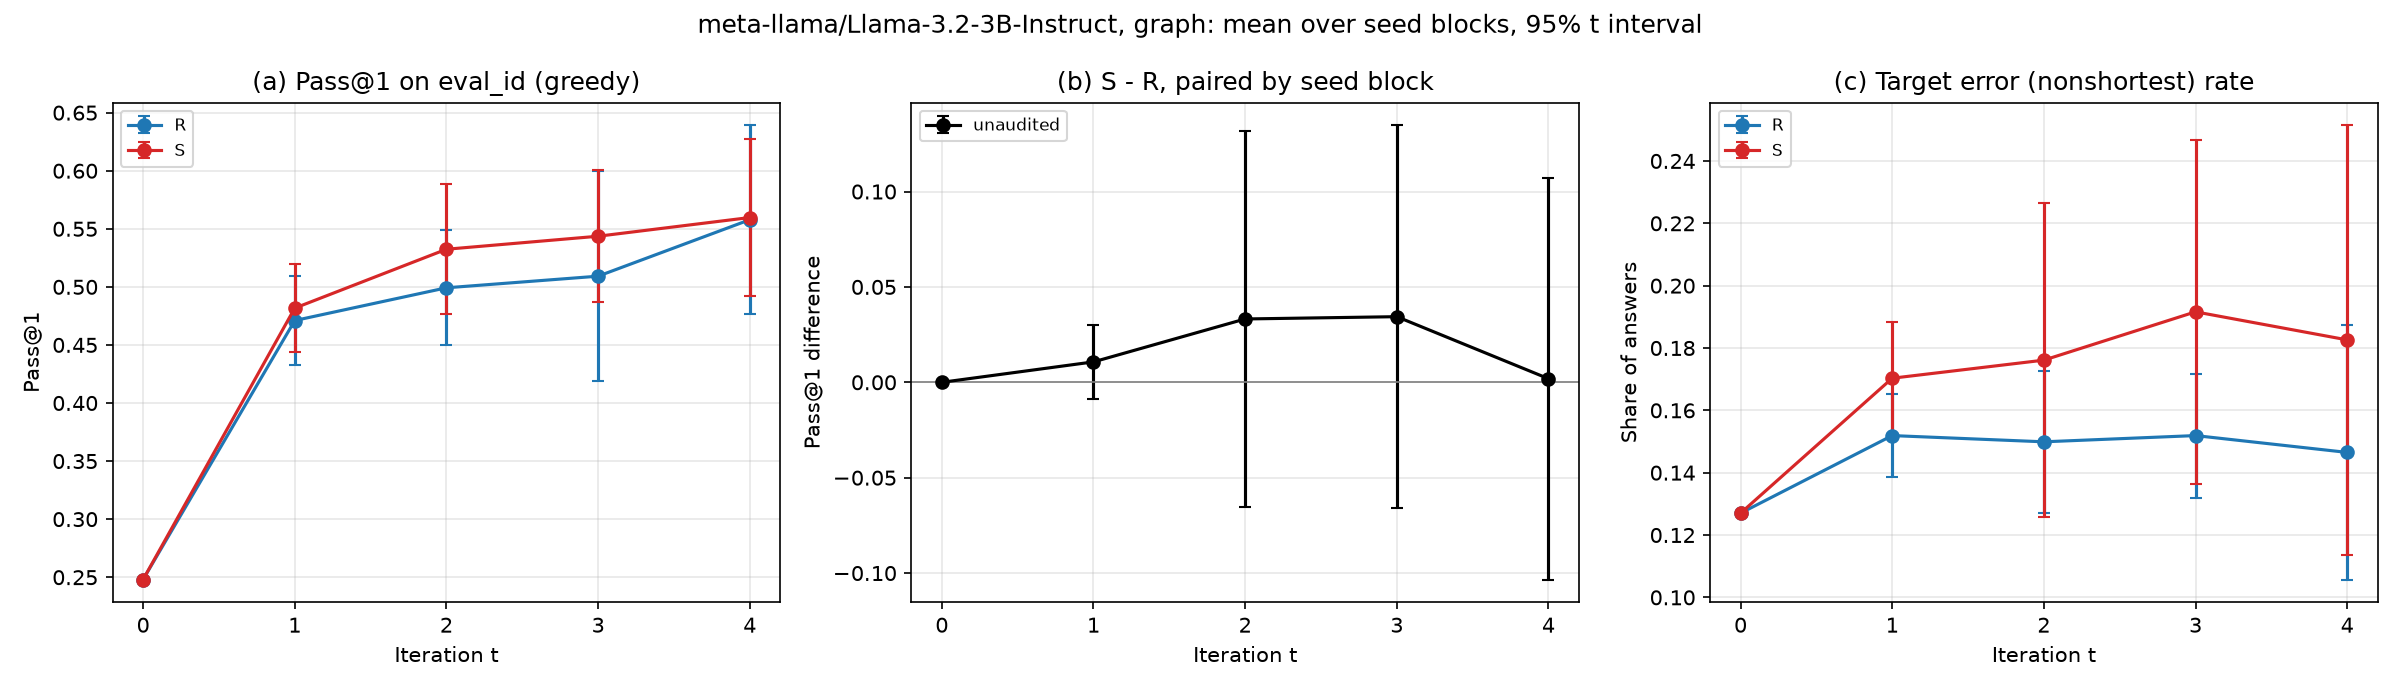
\includegraphics[width=0.90\linewidth]{figures/llama_four_round_raw/unaudited_eval_id_pass1.png}
\par\smallskip
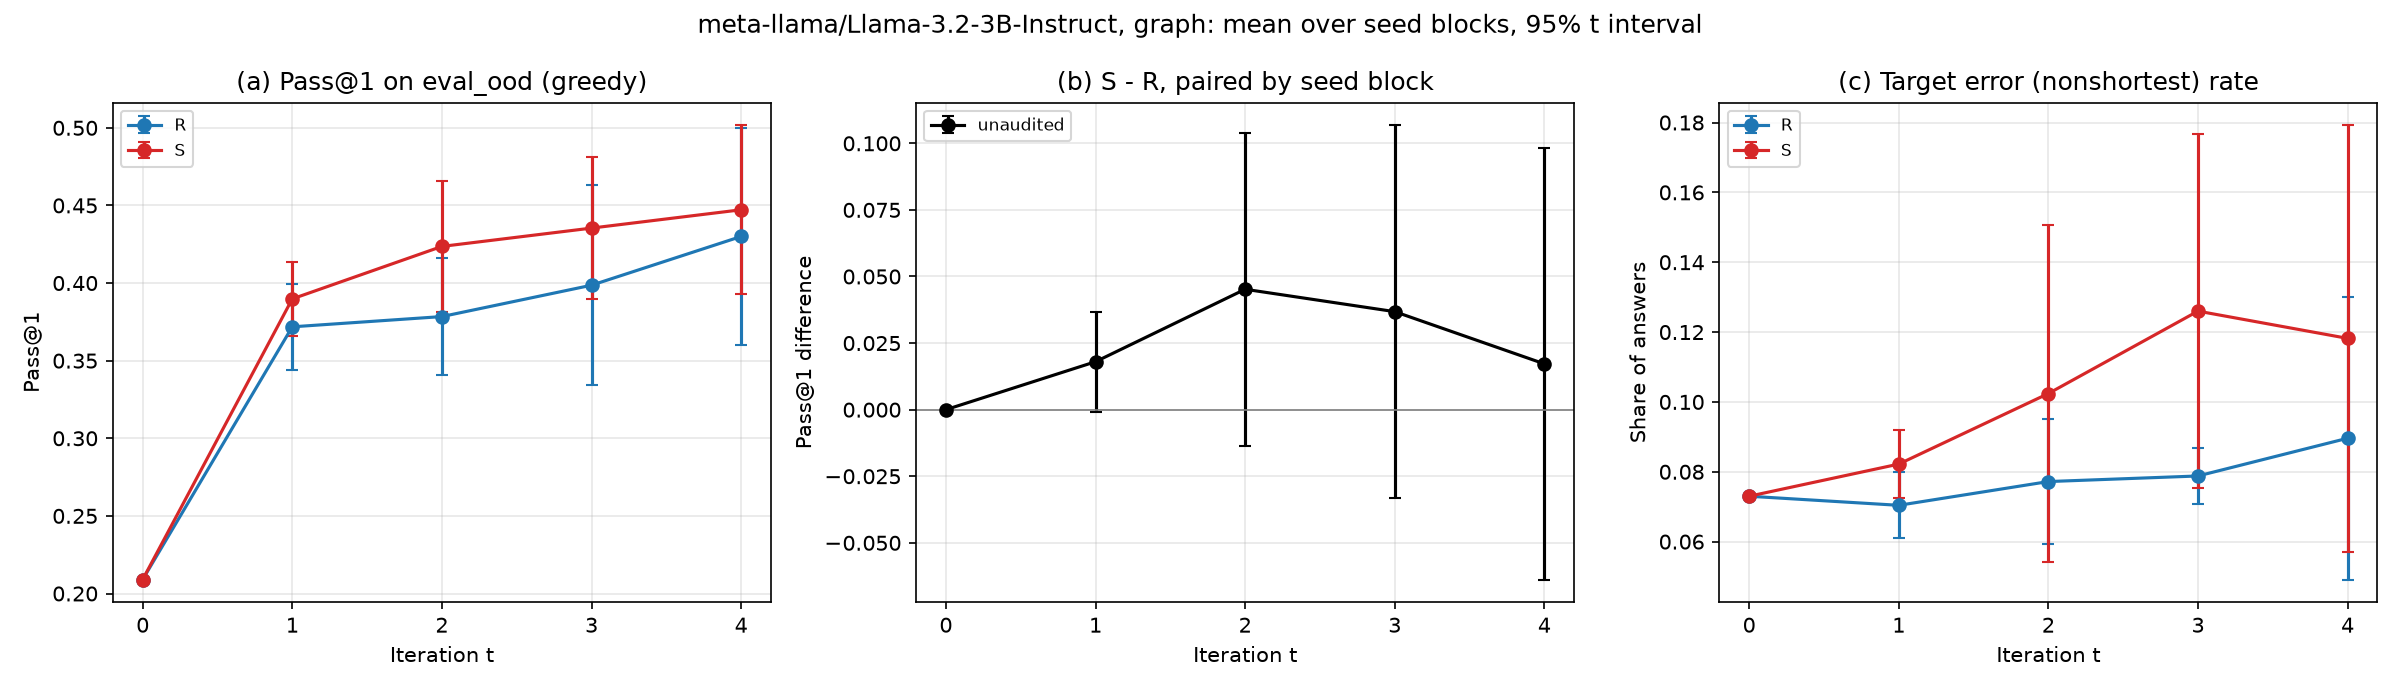
\includegraphics[width=0.90\linewidth]{figures/llama_four_round_raw/unaudited_eval_ood_pass1.png}
\caption{Original unaudited Llama-3.2-3B graph curves, ID (top) and OOD
(bottom), for rounds 0--4. The three panels show greedy Pass@1, paired
$S-R$ accuracy, and nonshortest-error incidence among all answers.}
\label{fig:llama-raw-unaudited}
\end{figure}

Both unaudited arms improve from the shared bases $0.248$ ID and
$0.209$ OOD. Round-four $R/S$ accuracy is $0.558/0.560$ ID and
$0.430/0.447$ OOD, with paired contrasts $0.002\pm0.105$ and
$0.017\pm0.081$.

\begin{figure}[H]
\centering
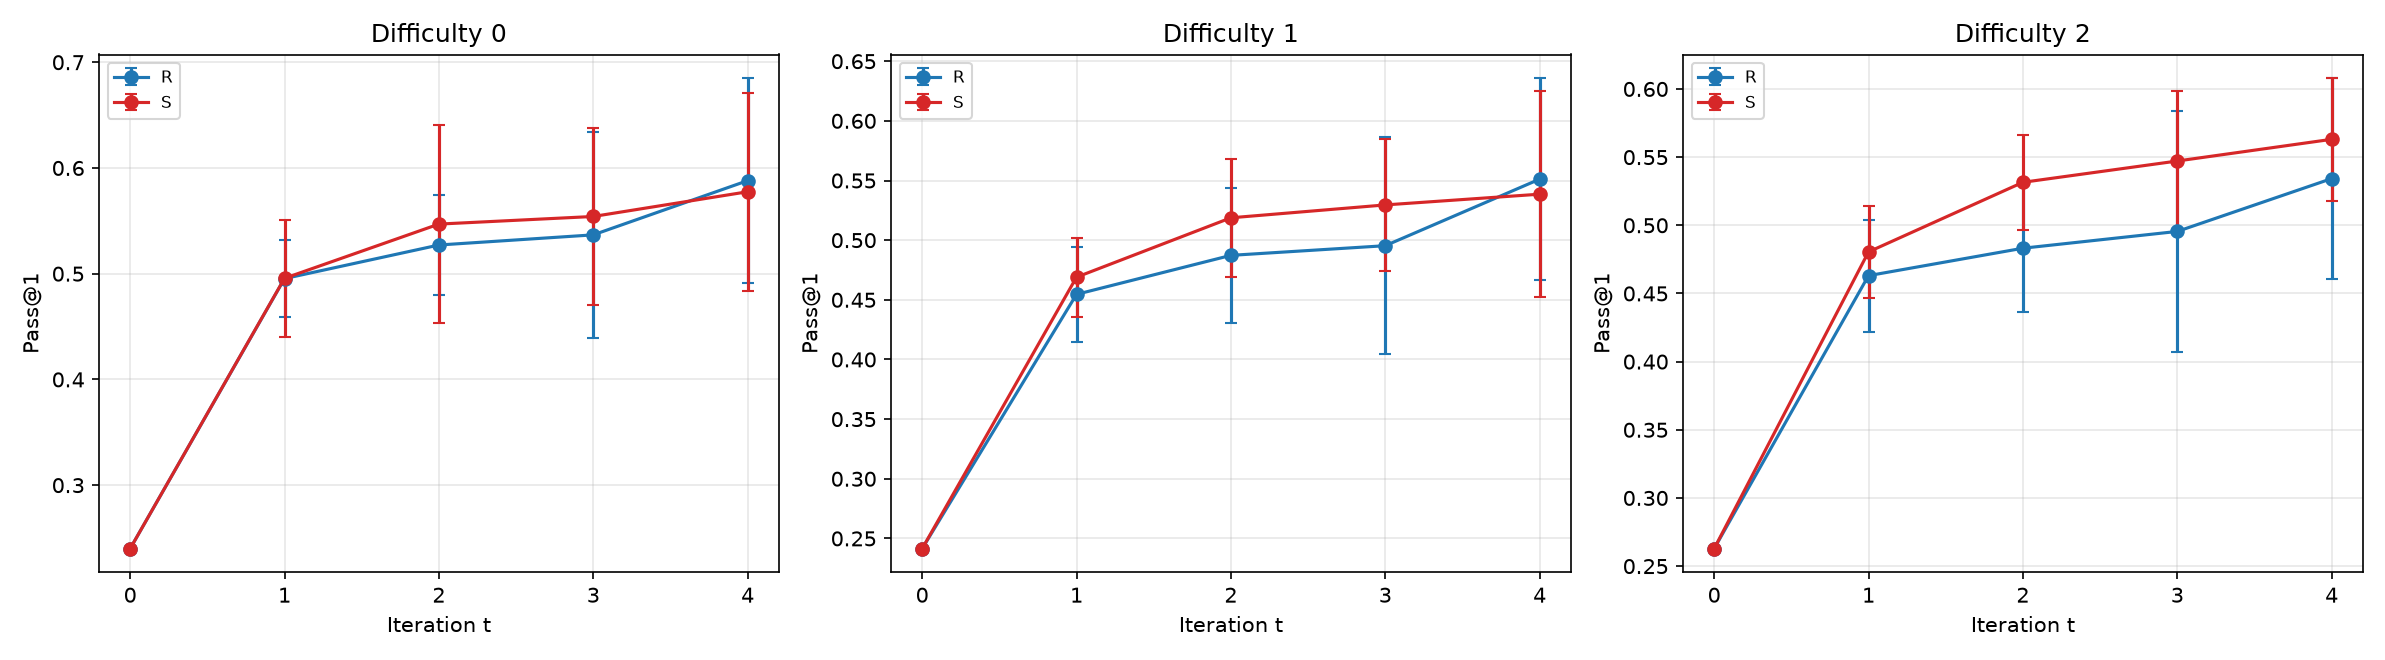
\includegraphics[width=0.90\linewidth]{figures/llama_four_round_raw/unaudited_eval_id_by_difficulty.png}
\par\smallskip
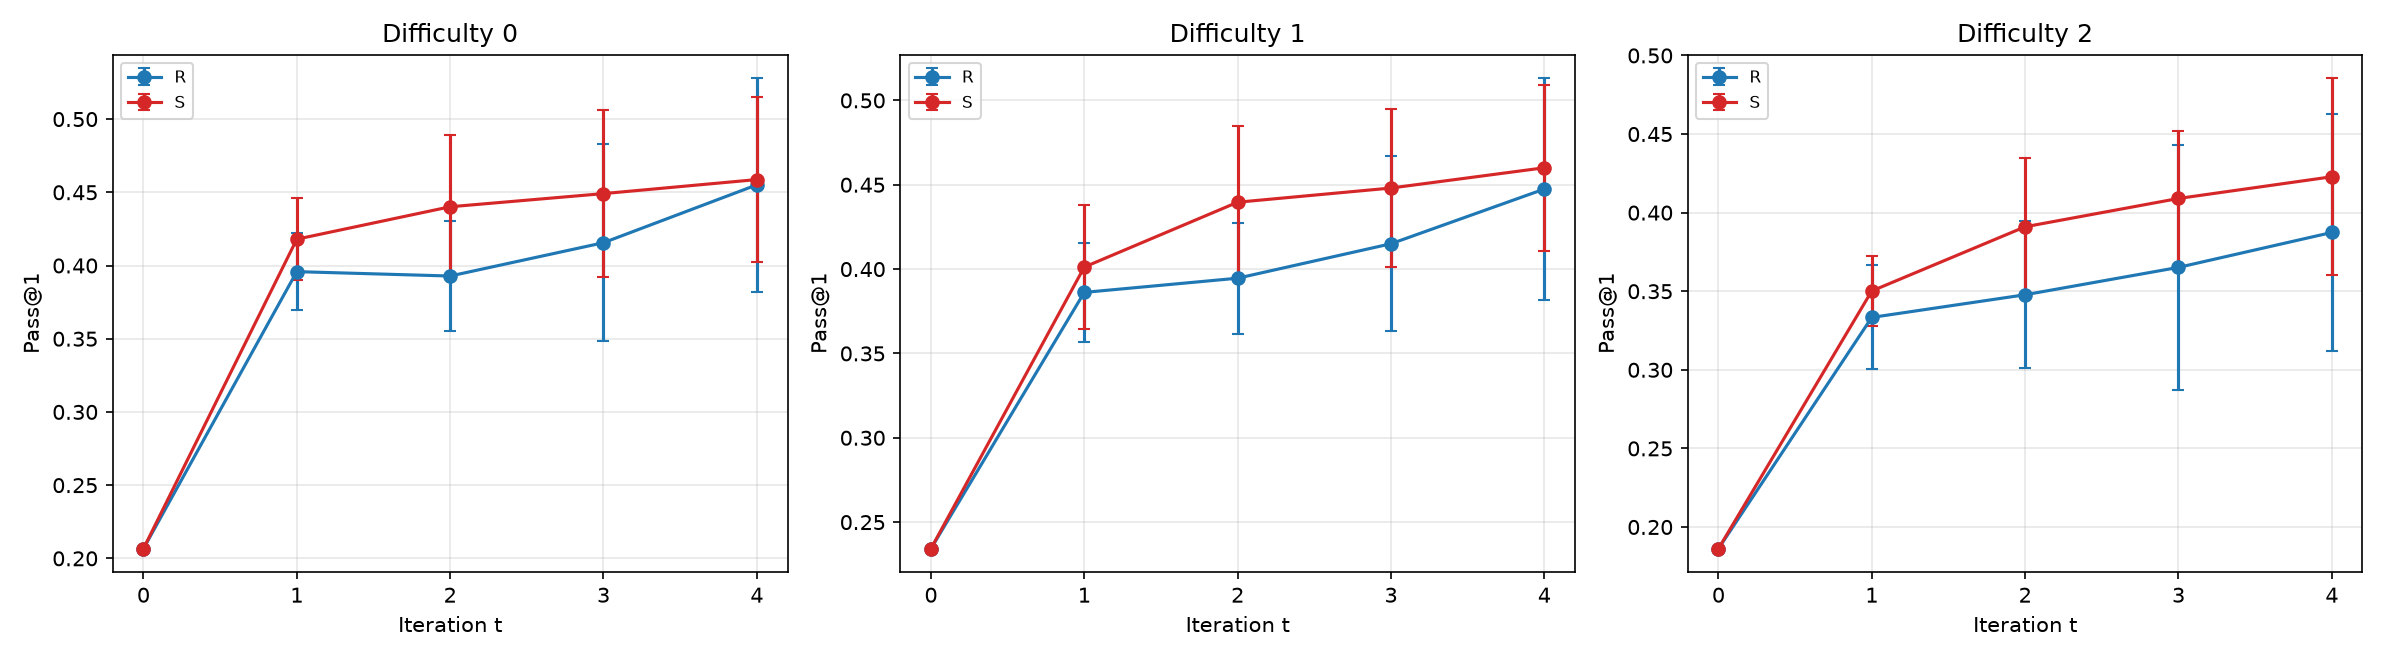
\includegraphics[width=0.90\linewidth]{figures/llama_four_round_raw/unaudited_eval_ood_by_difficulty.png}
\caption{Original unaudited Llama-3.2-3B graph accuracy by generator
difficulty stratum, ID (top) and OOD (bottom), for rounds 0--4.
Strata 0--2 run from left to right and contain $667/667/666$ ID
and $334/333/333$ OOD questions. Error bars use five paired blocks.}
\label{fig:llama-raw-unaudited-difficulty}
\end{figure}

These are fixed generator strata, not an established model-difficulty
ordering. The panel-specific vertical scales are retained, and differences
in the appearance of the curves do not constitute additional
difficulty-specific significance evidence.

\begin{figure}[H]
\centering
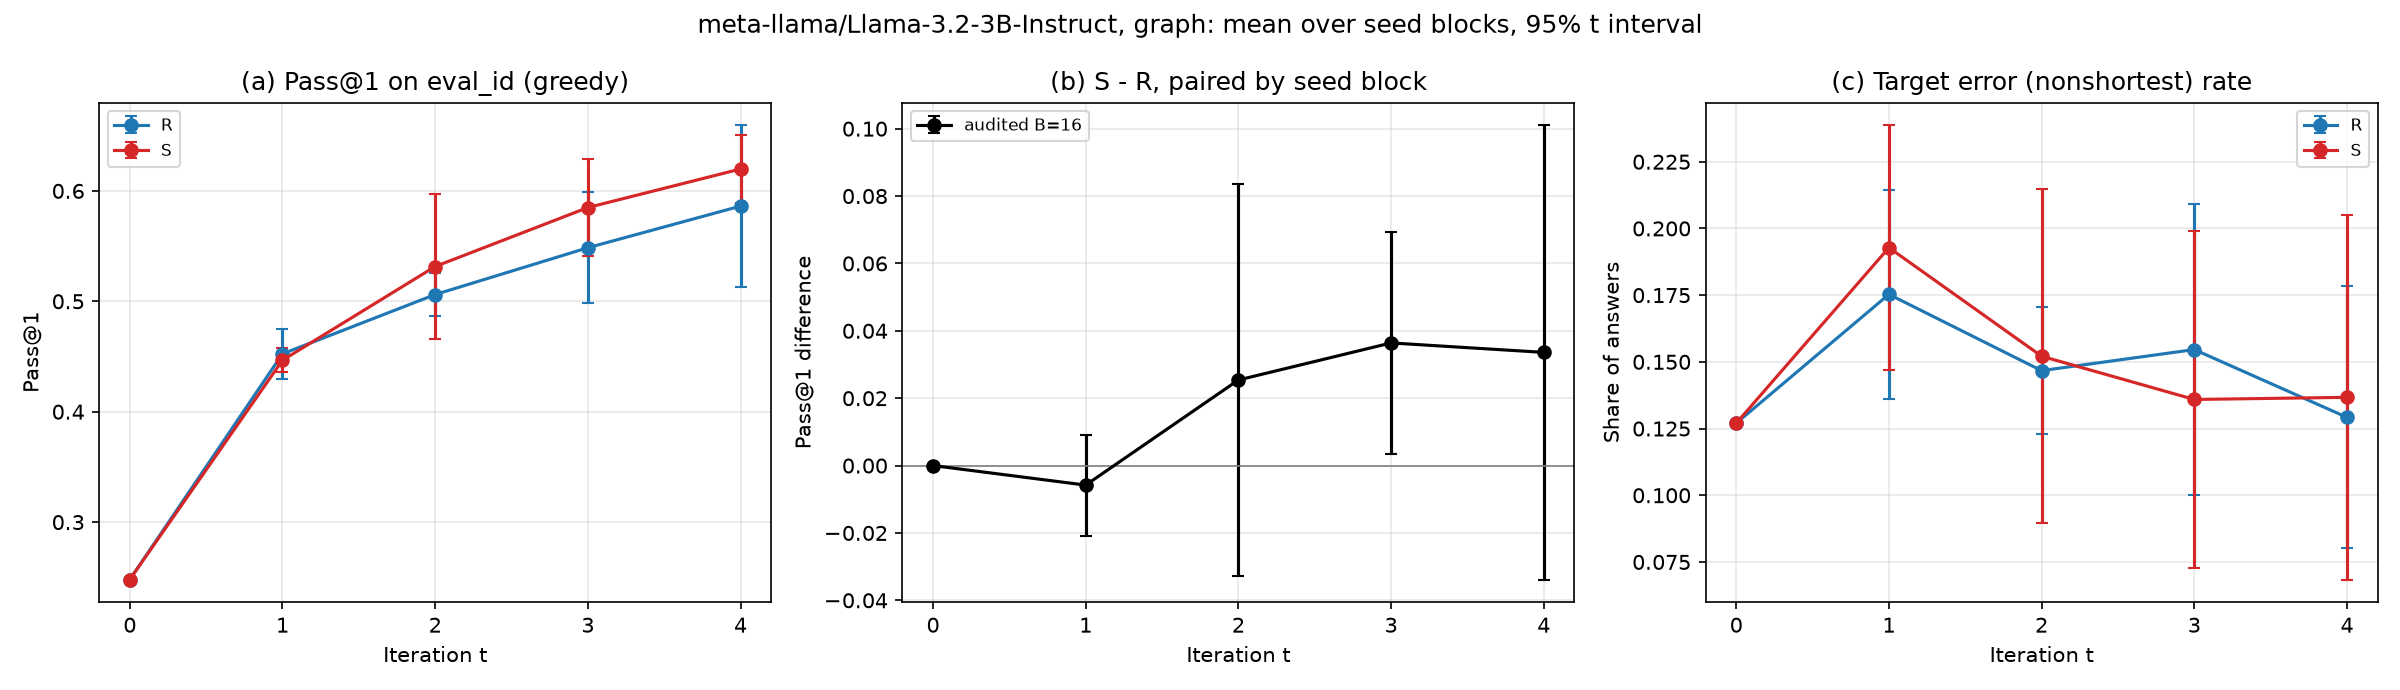
\includegraphics[width=0.90\linewidth]{figures/llama_four_round_raw/audited_eval_id_pass1.png}
\par\smallskip
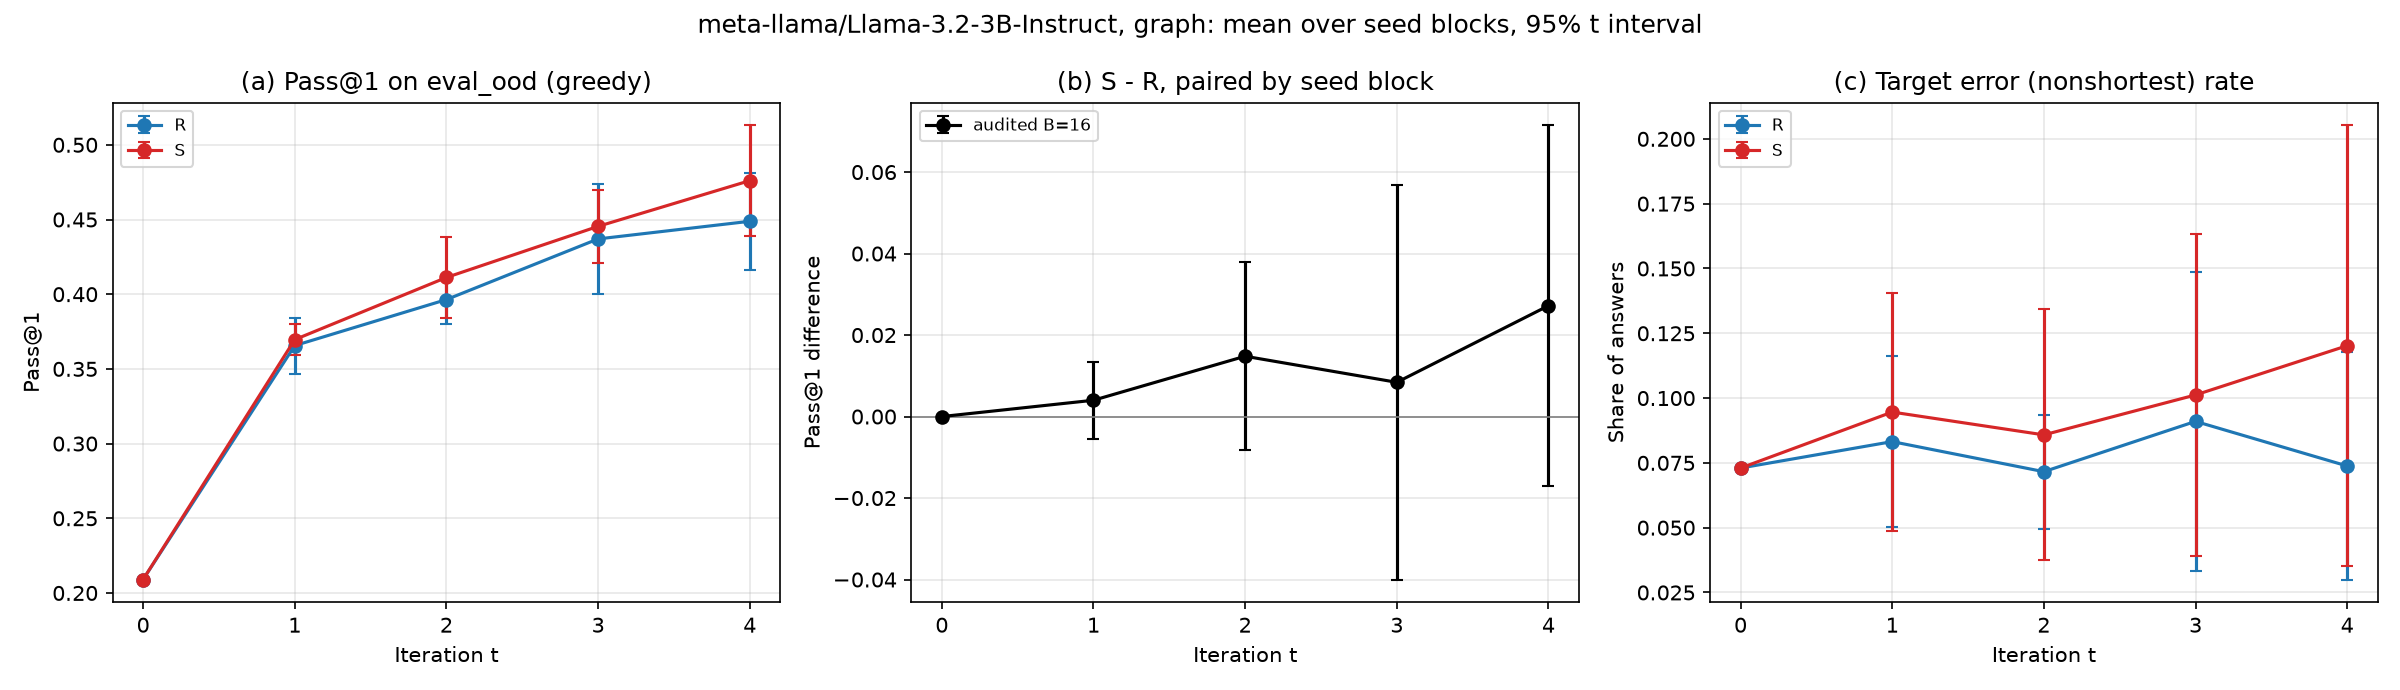
\includegraphics[width=0.90\linewidth]{figures/llama_four_round_raw/audited_eval_ood_pass1.png}
\caption{Original adaptive-audit Llama-3.2-3B graph curves, ID (top)
and OOD (bottom), with $B_{\rm qry}=16$ correctness queries per
arm-round. The panels show greedy Pass@1, paired $S-R$ accuracy,
and nonshortest-error incidence. Each audited arm spends 64 queries.}
\label{fig:llama-raw-audited}
\end{figure}

Audited round-four $R/S$ accuracy reaches $0.586/0.620$ ID and
$0.449/0.476$ OOD. The paired accuracy contrasts are
$0.034\pm0.067$ and $0.027\pm0.044$, respectively.
These are within-policy arm contrasts, not effects of auditing.

\begin{figure}[H]
\centering
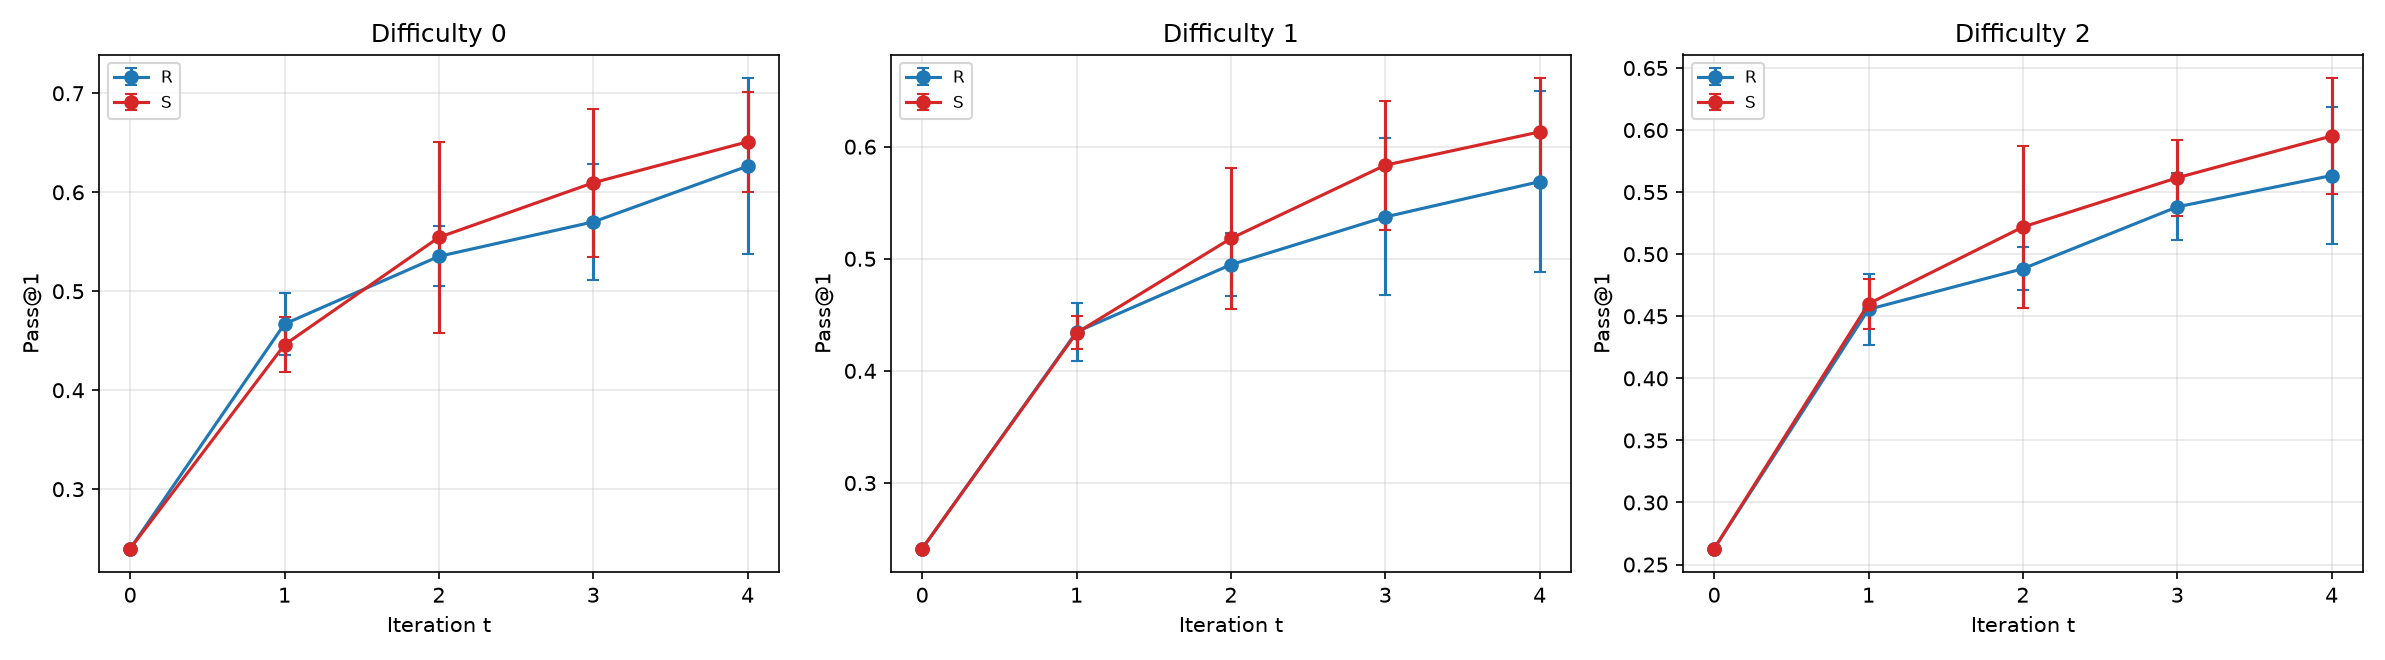
\includegraphics[width=0.90\linewidth]{figures/llama_four_round_raw/audited_eval_id_by_difficulty.png}
\par\smallskip
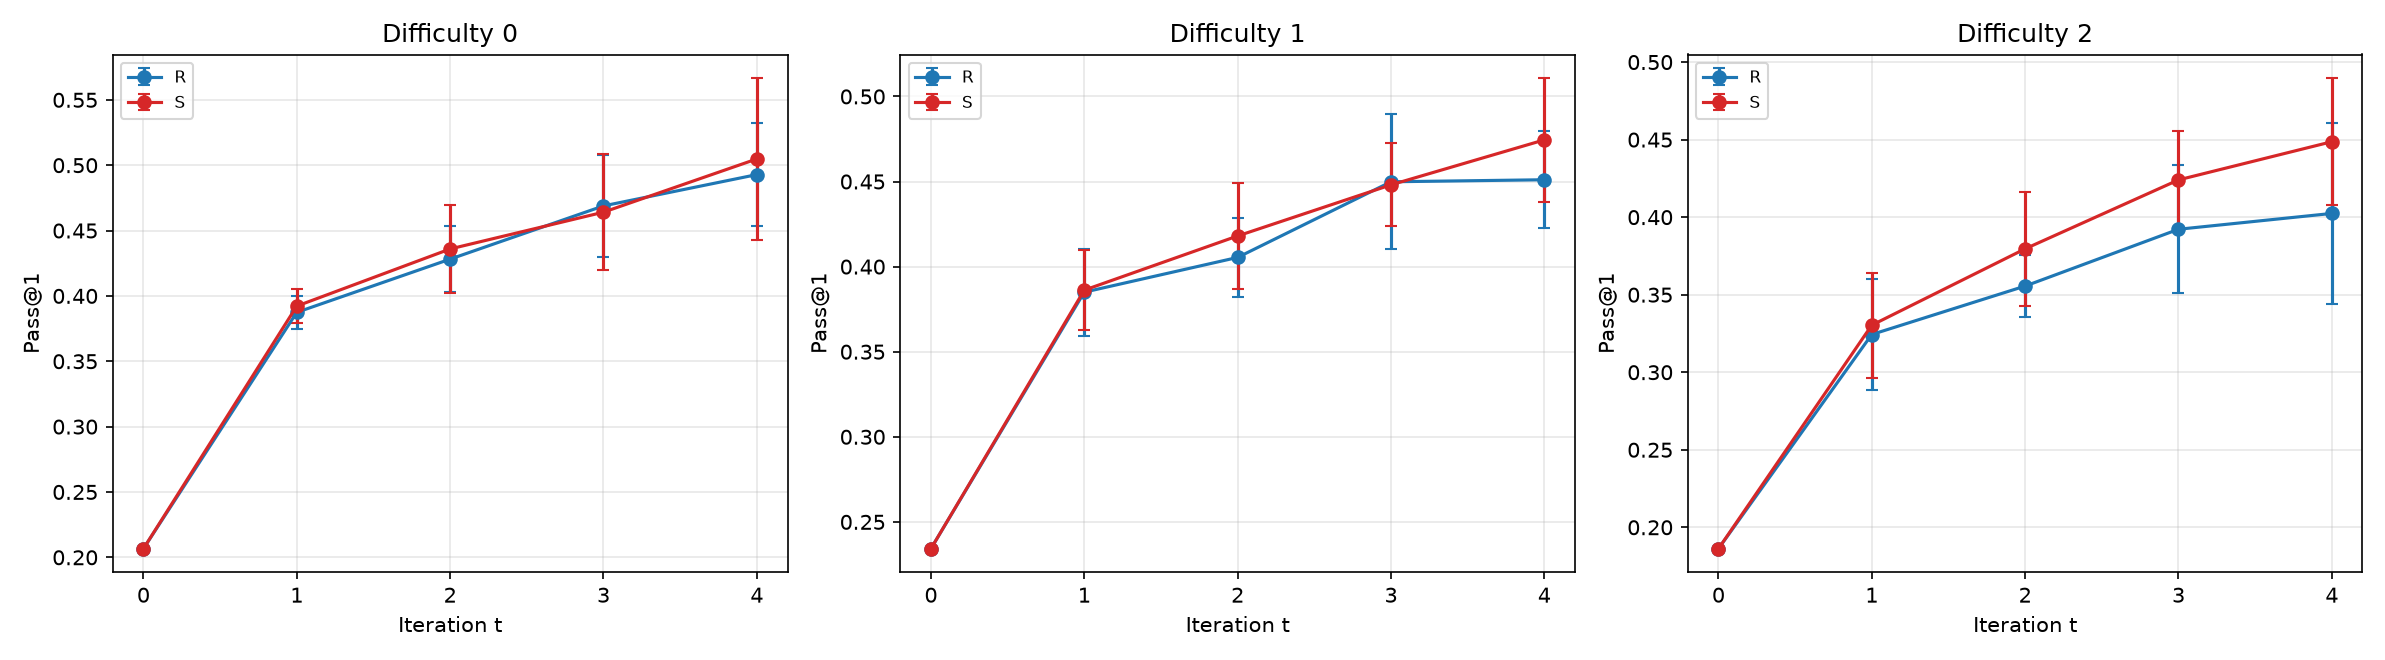
\includegraphics[width=0.90\linewidth]{figures/llama_four_round_raw/audited_eval_ood_by_difficulty.png}
\caption{Original adaptive-audit Llama-3.2-3B graph accuracy by
generator stratum, ID (top) and OOD (bottom), for rounds 0--4.
The fixed question strata and pointwise block-$t$ intervals follow
Figure~\ref{fig:llama-raw-unaudited-difficulty}.}
\label{fig:llama-raw-audited-difficulty}
\end{figure}

The audited curves show heterogeneous trajectories across the generator
strata. They retain separate vertical scales and use the same question
sets as the unaudited curves. This descriptive breakdown does not
establish stratum-specific audit benefits.

\begin{figure}[H]
\centering
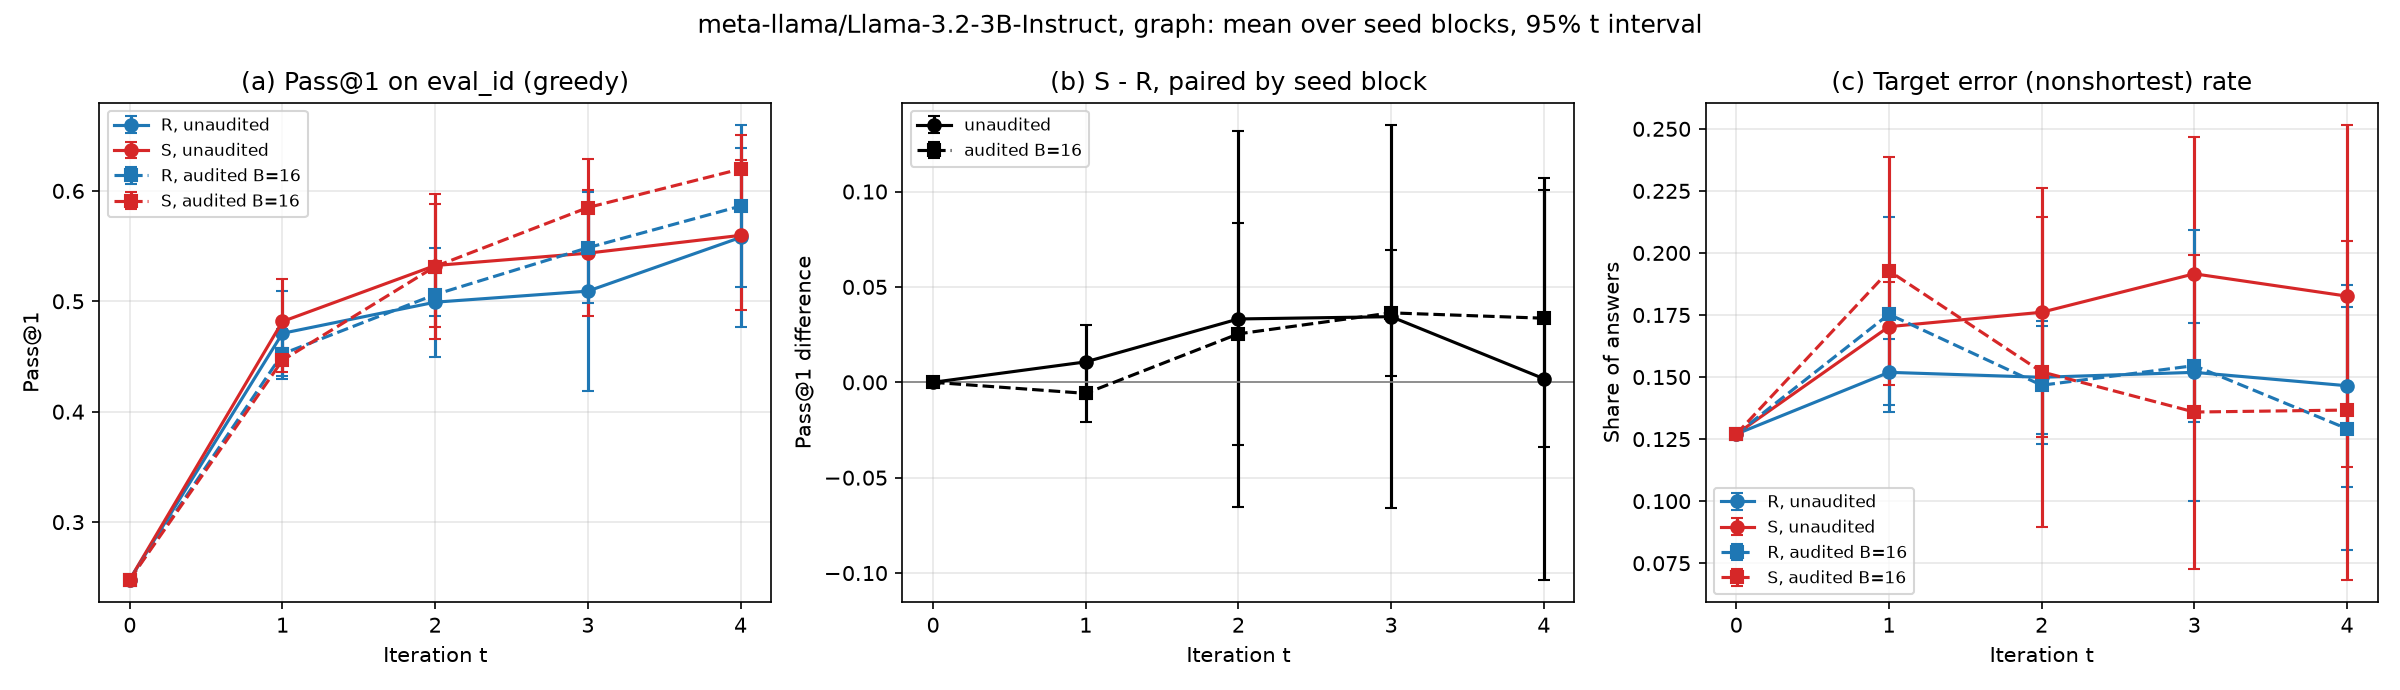
\includegraphics[width=0.90\linewidth]{figures/llama_four_round_raw/comparison_eval_id_pass1.png}
\par\smallskip
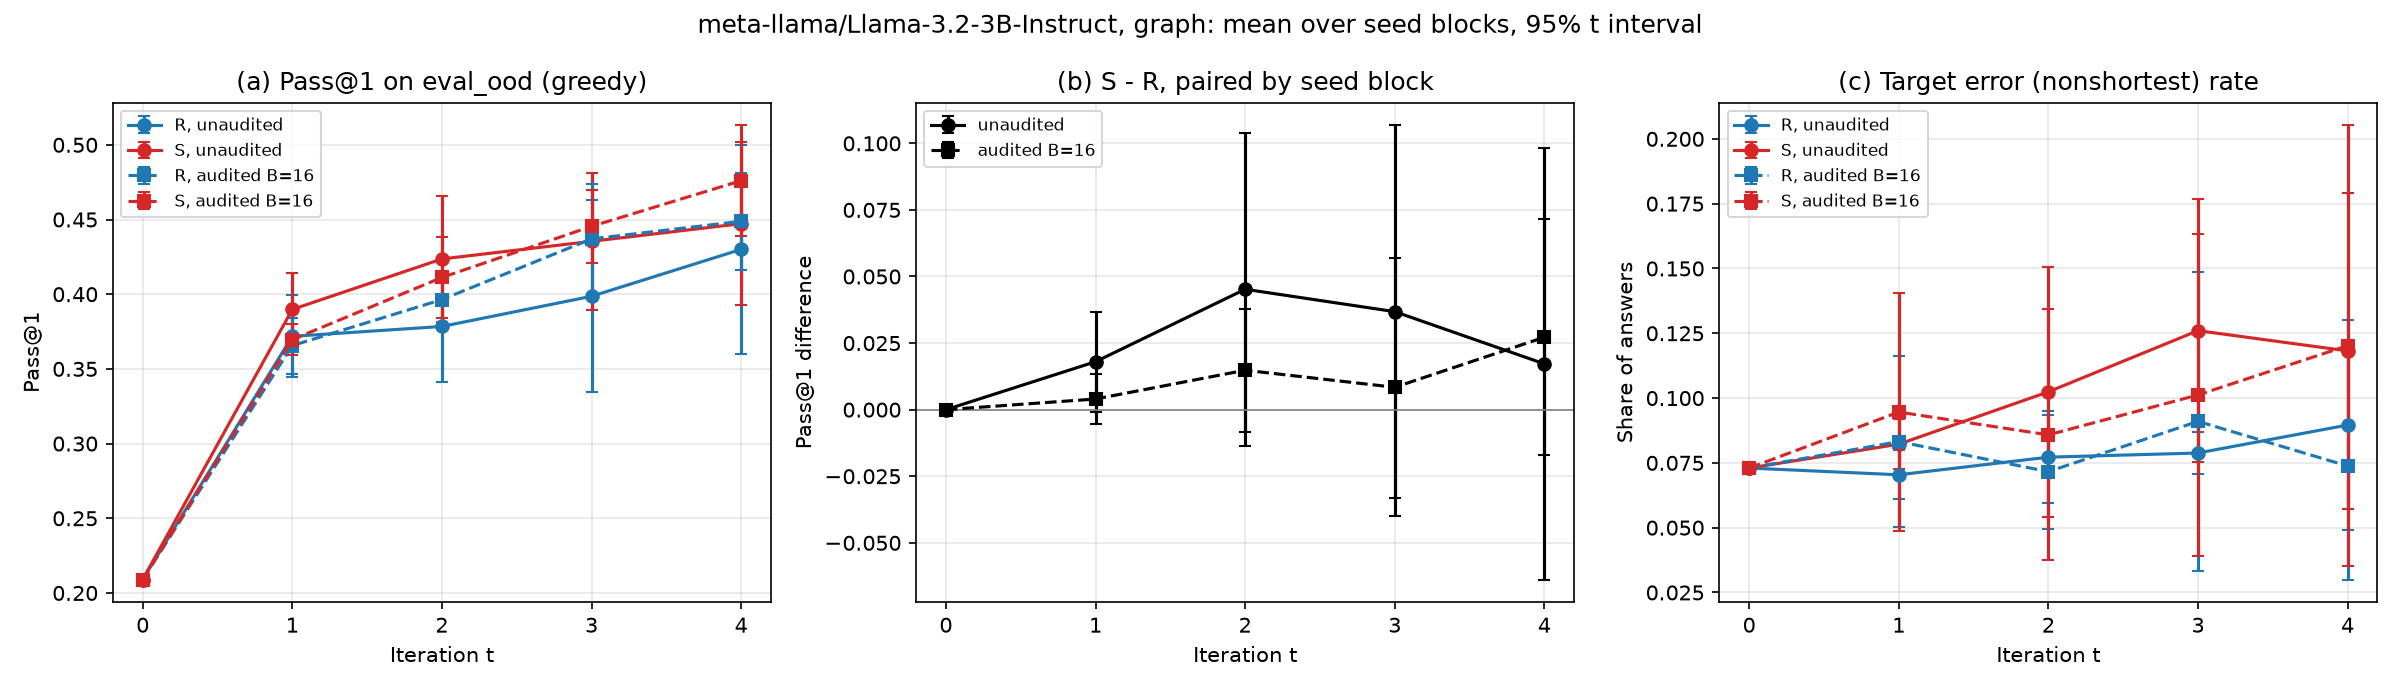
\includegraphics[width=0.90\linewidth]{figures/llama_four_round_raw/comparison_eval_ood_pass1.png}
\caption{Original joint comparison of unaudited and adaptive-audit
Llama-3.2-3B graph trajectories, ID (top) and OOD (bottom), for
rounds 0--4. Each middle panel reports paired $S-R$ accuracy
within each policy, not audited-minus-unaudited effects.}
\label{fig:llama-raw-comparison}
\label{fig:h100-id}
\label{fig:h100-ood}
\end{figure}

Auditing improves same-arm endpoint accuracy in mean
(Table~\ref{tab:audit-results}). Audited
OOD $S$ nonshortest incidence is $0.120$, versus $0.118$ without
auditing, so target-error suppression is not uniform.

\begin{figure}[H]
\centering
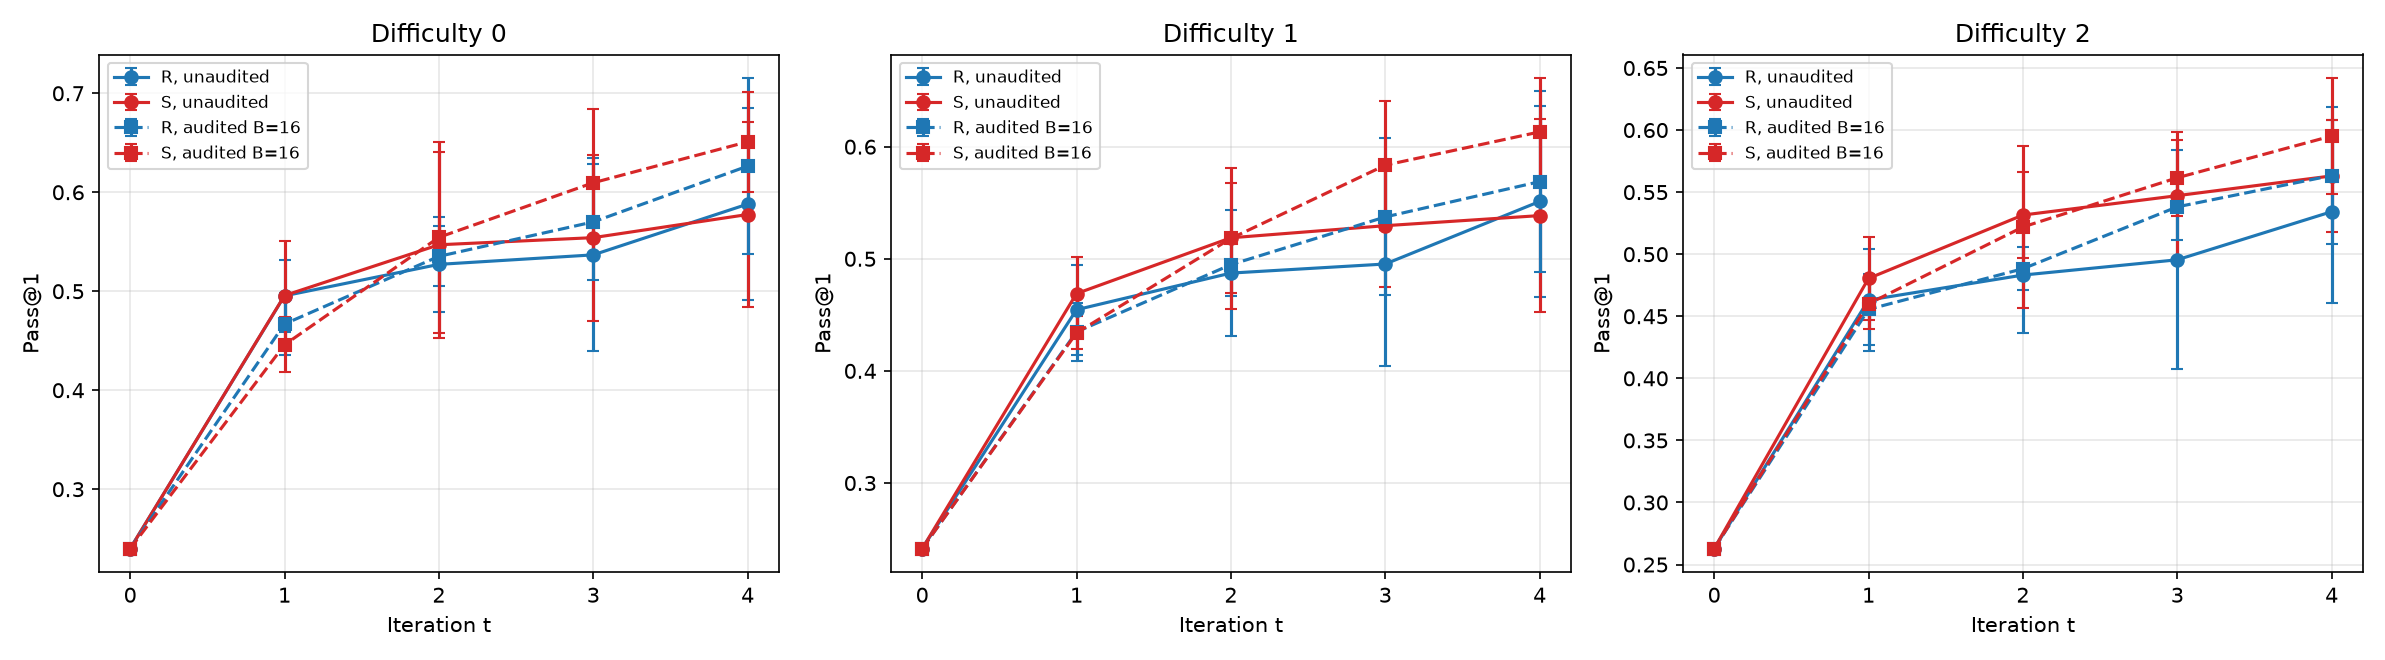
\includegraphics[width=0.90\linewidth]{figures/llama_four_round_raw/comparison_eval_id_by_difficulty.png}
\par\smallskip
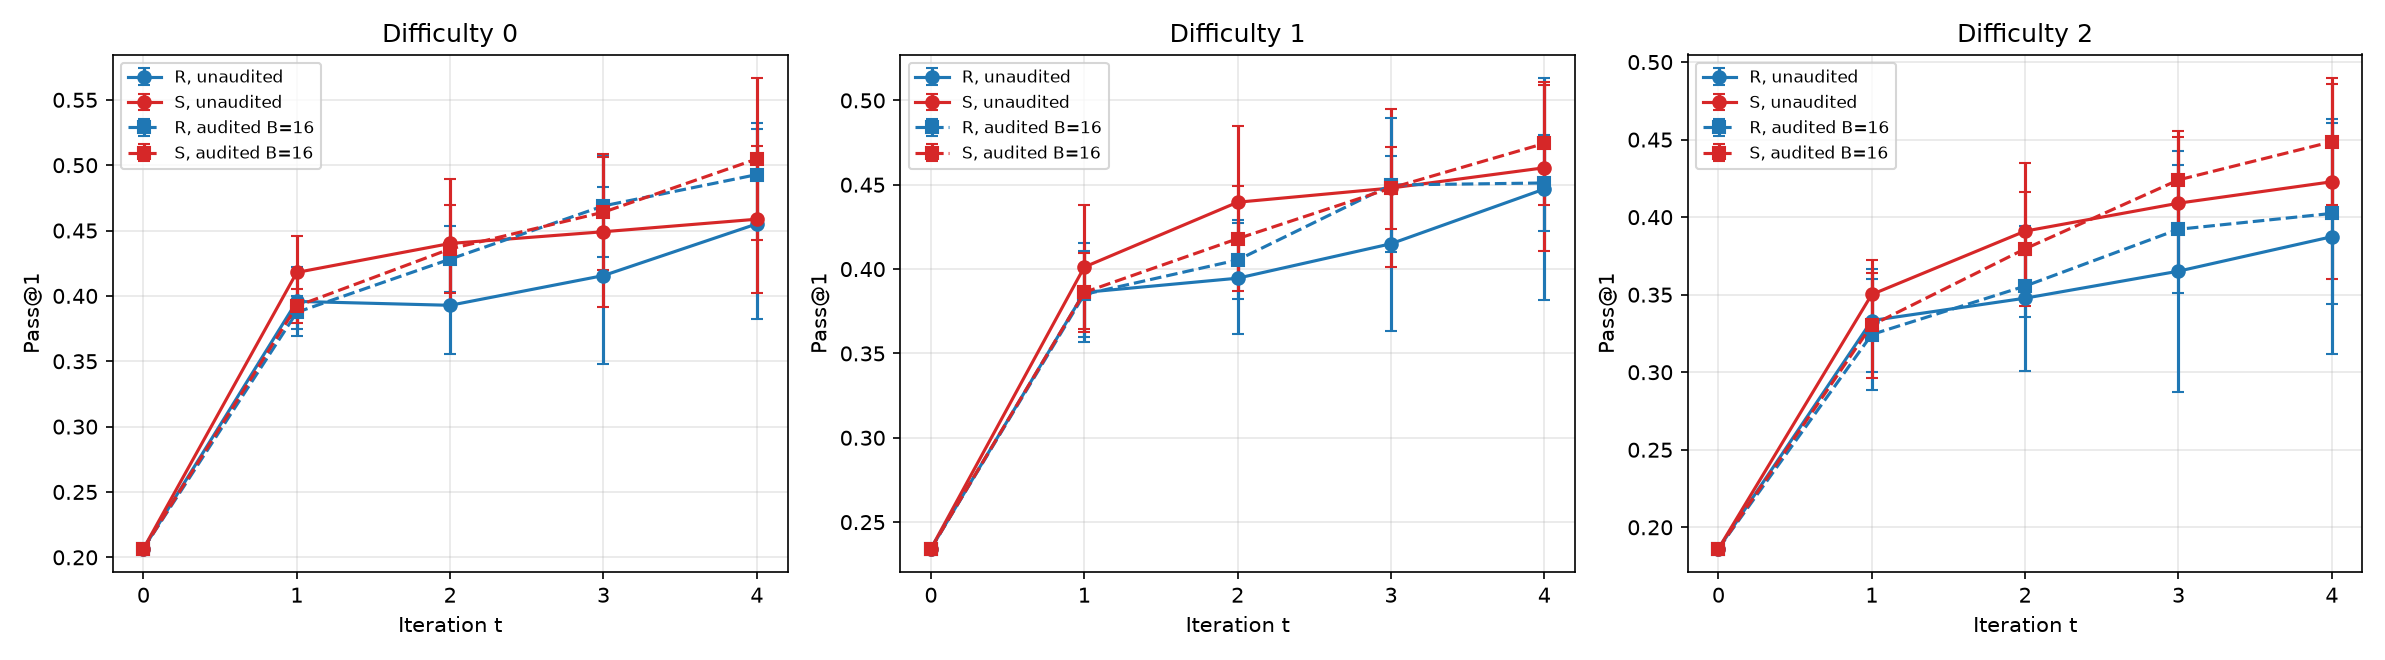
\includegraphics[width=0.90\linewidth]{figures/llama_four_round_raw/comparison_eval_ood_by_difficulty.png}
\caption{Original joint Llama-3.2-3B graph accuracy curves by
generator stratum, ID (top) and OOD (bottom), for rounds 0--4.
Both policies and both arms use the same question stratum at
each checkpoint. Counts and interval conventions follow
Figure~\ref{fig:llama-raw-unaudited-difficulty}.}
\label{fig:llama-raw-comparison-difficulty}
\label{fig:h100-difficulty}
\end{figure}

Both policies and both arms share the same question stratum at each
checkpoint. Separate vertical scales are retained, and the intervals
are not adjusted for comparisons across strata, rounds, or policies.
The joint curves complement the aggregate audit comparison without
providing an additional multiplicity-adjusted test.
\endgroup


\subsection{Shared audit and diagnostic conventions}
The finite-budget comparisons report correctness queries separately from
matching and evaluation labels. Retained rows, positive-weight rows, and
ESS measure different aspects of the training distribution; none alone
fixes optimizer effort. Within-policy $S-R$ contrasts and same-arm
audited-minus-unaudited changes answer different questions and are reported
separately for each model. All projections use a fixed initial reference
gradient and are surrogate diagnostics, not certificates of held-out
improvement. The population theorem analyzes a different auditing policy
and provides no direct guarantee for these adaptive finite-budget runs.

\subsection{Cross-task feasibility}
Table~\ref{tab:h100-feasibility} reports every block's round-one
pool statistics and eligible error-role prompts. Graph has exact-length
feasibility at $K=64$. The two arithmetic configurations deliberately
disable response-length matching; their counterfactual checks
fail exact-length matching at every $K$ in the ladder. This is a reported
protocol difference, not a post-hoc claim of exact-length arithmetic matching.
Raw-pool correctness/target counts in this table are distinct from
Table~\ref{tab:matching}'s eligible-pool rate denominators.
The added Qwen3-4B rows use independently rejudged original pools, with
exact-length error-role eligibility taken from matching certificates.
The arithmetic reference responses are bare canonical
integers (2--4 supervised tokens), whereas prompts request worked solutions
ending in \texttt{Answer: N}; projections can therefore reflect format changes.
The completed one-step graph outcomes and diagnostics are reported in
Tables~\ref{tab:one-step-heldout} and~\ref{tab:one-step-diagnostics}.

\begin{table}[H]
\caption{Round-one feasibility across five model/task pairs; audited siblings reuse the same pools. Each block has 16,384 sampled answers. Correctness and target counts use the full raw pool; matching excludes cut responses. $J_E$ counts prompts eligible for error-role matching at error fraction $0.25$, with exact length ($J_E^{\rm exact}$) or configured tolerance ($J_E^{\rm cfg}$). Qwen3-4B pool labels are independently rejudged; its $J_E$ values come from matching certificates. Graph permits $K=64$ with exact lengths. Arithmetic disables length matching; its exact-length ladder fails at $K=64,32,16$. These are feasibility checks, not held-out learning results.}
\label{tab:h100-feasibility}
\centering\small\setlength{\tabcolsep}{4pt}
\begin{tabular}{@{}llccccccc@{}}
\toprule
Task/model & Block & Correct (\%) & Cut & Target & $J_E^{\rm exact}$ & $J_E^{\rm cfg}$ & Length & $K$\\
\midrule
Graph / Qwen3-1.7B & b00 & 50.31 & 27 & 2357 & 27 & 27 & exact & 64\\
Graph / Qwen3-1.7B & b01 & 50.60 & 29 & 2351 & 38 & 38 & exact & 64\\
Graph / Qwen3-1.7B & b02 & 50.43 & 33 & 2322 & 32 & 32 & exact & 64\\
Graph / Qwen3-1.7B & b03 & 50.83 & 30 & 2354 & 31 & 31 & exact & 64\\
Graph / Qwen3-1.7B & b04 & 50.50 & 29 & 2346 & 28 & 28 & exact & 64\\
Graph / Llama-3B & b00 & 23.49 & 147 & 2095 & 184 & 184 & exact & 64\\
Graph / Llama-3B & b01 & 23.66 & 138 & 2112 & 180 & 180 & exact & 64\\
Graph / Llama-3B & b02 & 23.22 & 121 & 2095 & 178 & 178 & exact & 64\\
Graph / Llama-3B & b03 & 23.25 & 153 & 2140 & 188 & 188 & exact & 64\\
Graph / Llama-3B & b04 & 23.43 & 132 & 2124 & 192 & 192 & exact & 64\\
Arithmetic / Llama-3B & b00 & 74.48 & 0 & 74 & 2 & 30 & off & 64\\
Arithmetic / Llama-3B & b01 & 74.78 & 0 & 81 & 2 & 32 & off & 64\\
Arithmetic / Llama-3B & b02 & 74.71 & 2 & 71 & 1 & 17 & off & 64\\
Arithmetic / Llama-3B & b03 & 74.66 & 0 & 74 & 0 & 28 & off & 64\\
Arithmetic / Llama-3B & b04 & 74.83 & 2 & 87 & 1 & 33 & off & 64\\
Arithmetic / Llama-1B & b00 & 42.35 & 100 & 69 & 1 & 54 & off & 64\\
Arithmetic / Llama-1B & b01 & 42.03 & 111 & 69 & 2 & 45 & off & 64\\
Arithmetic / Llama-1B & b02 & 42.13 & 84 & 63 & 2 & 43 & off & 64\\
Arithmetic / Llama-1B & b03 & 42.30 & 90 & 75 & 2 & 55 & off & 64\\
Arithmetic / Llama-1B & b04 & 41.75 & 87 & 70 & 0 & 48 & off & 64\\
\addlinespace
Graph / Qwen3-4B & b00 & 63.02 & 9 & 3545 & 16 & 16 & exact & 64\\
Graph / Qwen3-4B & b01 & 63.01 & 7 & 3561 & 25 & 25 & exact & 64\\
Graph / Qwen3-4B & b02 & 63.23 & 10 & 3530 & 21 & 21 & exact & 64\\
Graph / Qwen3-4B & b03 & 63.29 & 5 & 3523 & 30 & 30 & exact & 64\\
Graph / Qwen3-4B & b04 & 63.02 & 9 & 3531 & 30 & 30 & exact & 64\\
\bottomrule
\end{tabular}
\end{table}


\subsection{Validation scope}
We independently reconstruct numerical summaries and figures from the
saved count and scalar records. The checks cover experiment completion,
shared initial pools and adapters, round-one matching constraints and
acceptance rates, checkpoint error counts and difficulty aggregation,
evaluation-protocol consistency, query and optimizer-step accounting,
and agreement with the plotting summaries. Overlapping Llama held-out
records agree across the initial and extended graph studies.
For the initial series, these checks do not independently rejudge responses,
reload checkpoints, or reconstruct unavailable gradient tensors and weights.
Qwen3-4B validation additionally rejudges original pools and audited held-out
answers, as detailed in Section~\ref{app:qwen4b-four-round}.

\subsection{Roundwise pre- and post-audit true-positive rates}
\label{app:roundwise-tpr}
Table~\ref{tab:h100-tpr} reports all four rounds of the completed graph
comparison. For each block, condition, arm, and round, $N^+$ counts correct
responses in that round's original pool after excluding truncated responses.
The pre-audit, retained, and positive-weight rates are
\[
 \mathrm{TPR}_{\rm pre}=\frac{48}{N^+},\qquad
 \mathrm{TPR}_{\rm ret}=\frac{C'}{N^+},\qquad
 \mathrm{TPR}_{w>0}=\frac{C'_{w>0}}{N^+},
\]
where $C'$ counts retained correct responses and $C'_{w>0}$ counts those
with positive training weight, irrespective of its magnitude. Auditing
keeps the same denominator.
All 40 audited arm-rounds retain the 48 selected correct responses, so
$\mathrm{TPR}_{\rm ret}=\mathrm{TPR}_{\rm pre}$; reliability weighting can
nevertheless reduce $\mathrm{TPR}_{w>0}$. In unaudited runs, unit weights
make selection TPR equal to positive-weight TPR.

Later pools come from each arm's preceding checkpoint, so their $N^+$
and TPRs need not agree across arms or conditions. With the correct quota
fixed at 48, a larger correct pool lowers selection TPR without implying
lower model accuracy. These rates are distinct from subset precision and
held-out Pass@1. We check block-level numerators and denominators for
80 completed arm-rounds and 40 audit reports. This establishes consistency
of the saved counts, not independent rejudging of unavailable raw responses.

The Llama rates are collected with its other four-round results in
Table~\ref{tab:h100-tpr}; Qwen rates appear in
Tables~\ref{tab:qwen-audit} and~\ref{tab:qwen4b-audit}.
\subsection{Qwen3-1.7B: four-round graph replication}
\label{app:qwen-four-round}

The Qwen3-1.7B unaudited and adaptive-audit graph comparisons each have
five complete paired blocks and both held-out splits. The primary analysis
uses the fixed rounds 0--4 horizon; round-eight contrasts are reported at
the end of this subsection, without selecting a best checkpoint.

Qwen3-1.7B response generation uses temperature $1.3$ and
top-$p=1$. LoRA, matching quotas, optimizer settings, prompt/sample counts,
and audit budget follow the four-round protocol in Section~\ref{sec:experiments}.
There are 40 trained checkpoints per policy in the selected horizon,
plus one shared base, each evaluated greedily on 2,000 ID and 1,000 OOD
questions. Policies bind the same initial adapter, dataset, and round-one
pools. Table~\ref{tab:qwen-matching} reports the nontruncated-pool
TPR/FPR and exact initial matching controls; $R$ already contains 6--12
nonshortest errors among its 16 accepted errors.

\begin{table}[H]
\caption{Qwen3-1.7B graph round-one matching certificate, common to the audited and unaudited runs and their one-step reuse. $N^+/N^-$ exclude truncated answers; $R/S$ share correct IDs, task IDs, 48/16 correct/error quotas and exact supervised response lengths. Later checkpoint-dependent pools are not jointly matched.}
\label{tab:qwen-matching}
\centering\small\setlength{\tabcolsep}{3pt}
\begin{tabular}{@{}lllllll@{}}
\toprule
Block & $N^+/N^-$ & Cut & TPR/FPR & Yield & Target hits $R/S$ & Controls\\
\midrule
b00 & 8243/8114 & 27 & 0.005823/0.001972 & 0.003913 & 12/16 & pass\\
b01 & 8290/8065 & 29 & 0.005790/0.001984 & 0.003913 & 6/16 & pass\\
b02 & 8262/8089 & 33 & 0.005810/0.001978 & 0.003914 & 12/16 & pass\\
b03 & 8328/8026 & 30 & 0.005764/0.001994 & 0.003913 & 9/16 & pass\\
b04 & 8274/8081 & 29 & 0.005801/0.001980 & 0.003913 & 6/16 & pass\\
\bottomrule
\end{tabular}
\end{table}

\begin{table}[H]
\caption{Qwen3-1.7B graph endpoints after four rounds. Target rates count nonshortest answers among all evaluated questions. Paired differences use five blocks, with descriptive 95\% block-$t$ half-widths; no multiplicity adjustment is applied.}
\label{tab:qwen-endpoints}
\centering\small\setlength{\tabcolsep}{3pt}
\begin{tabular}{@{}lllllll@{}}
\toprule
Split & Policy & Base & Pass@1 $R/S$ & $S-R$ Pass@1 & Target $R/S$ & $S-R$ target\\
\midrule
ID & None & 0.4995 & 0.556/0.553 & $-0.003\pm0.044$ & 0.103/0.171 & $0.068\pm0.039$\\
ID & B=16 & 0.4995 & 0.533/0.551 & $0.017\pm0.093$ & 0.129/0.158 & $0.029\pm0.074$\\
OOD & None & 0.3470 & 0.363/0.389 & $0.026\pm0.038$ & 0.057/0.124 & $0.066\pm0.038$\\
OOD & B=16 & 0.3470 & 0.362/0.386 & $0.024\pm0.038$ & 0.073/0.102 & $0.029\pm0.043$\\
\bottomrule
\end{tabular}
\end{table}

\begin{table}[H]
\caption{Qwen3-1.7B four-round graph policy endpoints, with five paired blocks. Errors are mean fractions. $Q$ counts correctness-audit queries per arm/block, excluding matching and evaluation labels; steps are cumulative updates (mean and range). $\Delta$ is audited-minus-unaudited error with a descriptive paired 95\% block-$t$ interval on fixed questions (negative favors auditing). Models are not pooled. One-step outcomes are separate (Table~\ref{tab:one-step-heldout}).}
\label{tab:qwen17-policy-endpoints}
\centering\small\setlength{\tabcolsep}{3pt}
\begin{tabular}{@{}llcccccc@{}}
\toprule
Policy & Arm & $Q$ & Steps & ID error & OOD error & \shortstack{$\Delta$ID\\(95\% CI)} & \shortstack{$\Delta$OOD\\(95\% CI)}\\
\midrule
\multicolumn{8}{@{}l}{\textbf{Qwen3-1.7B}}\\
Base & --- & 0 & 0 & 0.5005 & 0.6530 & --- & ---\\
Unaudited & R & 0 & 64 & 0.444 & 0.637 & --- & ---\\
Unaudited & S & 0 & 64 & 0.447 & 0.611 & --- & ---\\
Adaptive, B=16 & R & 64 & 48.0 (37--56) & 0.467 & 0.638 & $0.022\;[-0.026,0.071]$ & $0.001\;[-0.037,0.039]$\\
Adaptive, B=16 & S & 64 & 53.2 (46--57) & 0.449 & 0.614 & $0.002\;[-0.082,0.086]$ & $0.003\;[-0.054,0.060]$\\
\bottomrule
\end{tabular}
\end{table}

\begin{figure}[H]
\centering
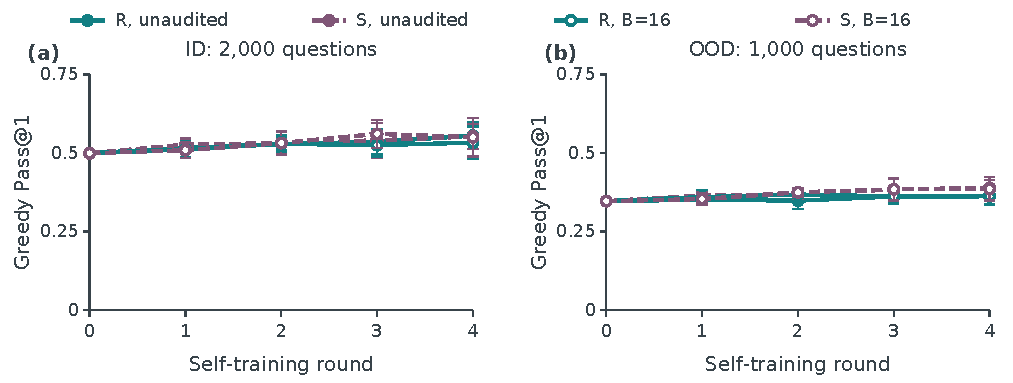
\includegraphics[width=0.8\linewidth]{figures/graph_extensions/qwen_accuracy.pdf}
\caption{Four-round Qwen3-1.7B graph self-training improves mean accuracy in both arms
from shared base accuracy $0.4995$ ID/$0.347$ OOD. Unaudited $R/S$ reach
$0.556/0.553$ ID and $0.363/0.389$ OOD; with 16 correctness queries per
arm-round, they reach $0.533/0.551$ and $0.362/0.386$, respectively.
Bars are pointwise 95\% block-$t$ intervals over five blocks on fixed
questions. Round zero has one shared checkpoint; only rounds 0--4 are shown.
Nonshortest-error incidence is reported in Figure~\ref{fig:qwen-target-errors}.}
\label{fig:qwen-four-round}
\end{figure}


\begin{figure}[H]
\centering
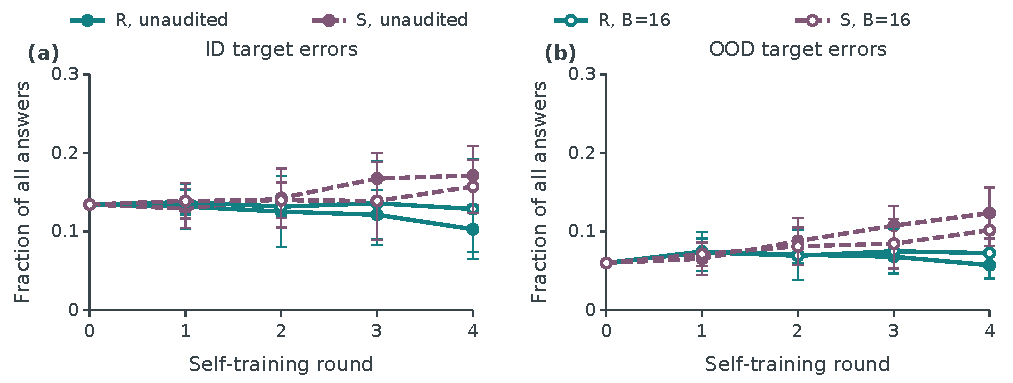
\includegraphics[width=0.8\linewidth]{figures/graph_extensions/qwen_target_errors.pdf}
\caption{Qwen3-1.7B four-round nonshortest-error incidence among all answers.
Unaudited $R/S$ reach $0.103/0.171$ ID and $0.057/0.124$ OOD at round four;
unaudited target-incidence contrasts are $0.068\pm0.039$ ID and $0.066\pm0.038$ OOD.
Audited target-incidence contrasts are $0.029\pm0.074$ ID and
$0.029\pm0.043$ OOD. Bars are
pointwise 95\% block-$t$ intervals over five blocks; the common base has
no independent block replication. Only rounds 0--4 are shown.}
\label{fig:qwen-target-errors}
\end{figure}

Accuracy and error composition need not tell the same story. In the
unaudited Qwen comparison, the round-four nonshortest fractions are
$0.103/0.171$ ID and $0.057/0.124$ OOD for $R/S$. Both paired target
contrasts have descriptive intervals above zero, despite accuracy
contrasts $-0.003\pm0.044$ ID and $0.026\pm0.038$ OOD. This is a
task-signature finding, not a measurement of high-influence errors or
the opposite-direction construction. The audited target contrasts are
$0.029\pm0.074$ ID and $0.029\pm0.043$ OOD.
All rounds and endpoint blocks appear in Tables~\ref{tab:qwen-rounds}
and~\ref{tab:qwen-blocks}. These multiple descriptive comparisons are
not multiplicity-adjusted confirmatory tests.

\begin{table}[H]
\caption{Qwen3-1.7B graph trajectories restricted to the original four-round protocol. Entries are means $\pm$ pointwise 95\% block-$t$ half-widths. The base is one common checkpoint, not five independent fits.}
\label{tab:qwen-rounds}
\centering\small\setlength{\tabcolsep}{3pt}
\begin{tabular}{@{}lllllllll@{}}
\toprule
Split & Policy & Round & Pass@1 $R$ & Pass@1 $S$ & Pass@1 $S-R$ & Target $R$ & Target $S$ & Target $S-R$\\
\midrule
ID & Base & 0 & 0.4995 & 0.4995 & --- & 0.135 & 0.135 & ---\\
ID & None & 1 & $0.517\pm0.017$ & $0.527\pm0.019$ & $0.010\pm0.012$ & $0.132\pm0.029$ & $0.129\pm0.024$ & $-0.003\pm0.012$\\
ID & None & 2 & $0.529\pm0.029$ & $0.532\pm0.037$ & $0.003\pm0.035$ & $0.126\pm0.045$ & $0.143\pm0.038$ & $0.017\pm0.043$\\
ID & None & 3 & $0.536\pm0.040$ & $0.541\pm0.055$ & $0.005\pm0.039$ & $0.121\pm0.031$ & $0.168\pm0.032$ & $0.046\pm0.022$\\
ID & None & 4 & $0.556\pm0.043$ & $0.553\pm0.040$ & $-0.003\pm0.044$ & $0.103\pm0.029$ & $0.171\pm0.037$ & $0.068\pm0.039$\\
ID & B=16 & 1 & $0.513\pm0.027$ & $0.509\pm0.024$ & $-0.003\pm0.017$ & $0.138\pm0.016$ & $0.139\pm0.022$ & $0.002\pm0.009$\\
ID & B=16 & 2 & $0.529\pm0.021$ & $0.532\pm0.012$ & $0.003\pm0.015$ & $0.132\pm0.014$ & $0.140\pm0.022$ & $0.008\pm0.020$\\
ID & B=16 & 3 & $0.526\pm0.039$ & $0.561\pm0.045$ & $0.036\pm0.056$ & $0.136\pm0.053$ & $0.139\pm0.049$ & $0.003\pm0.073$\\
ID & B=16 & 4 & $0.533\pm0.051$ & $0.551\pm0.062$ & $0.017\pm0.093$ & $0.129\pm0.064$ & $0.158\pm0.034$ & $0.029\pm0.074$\\
OOD & Base & 0 & 0.3470 & 0.3470 & --- & 0.060 & 0.060 & ---\\
OOD & None & 1 & $0.352\pm0.011$ & $0.366\pm0.015$ & $0.014\pm0.021$ & $0.075\pm0.025$ & $0.065\pm0.021$ & $-0.009\pm0.007$\\
OOD & None & 2 & $0.349\pm0.026$ & $0.369\pm0.016$ & $0.020\pm0.020$ & $0.071\pm0.032$ & $0.088\pm0.029$ & $0.017\pm0.026$\\
OOD & None & 3 & $0.362\pm0.022$ & $0.385\pm0.034$ & $0.023\pm0.022$ & $0.068\pm0.016$ & $0.108\pm0.025$ & $0.040\pm0.015$\\
OOD & None & 4 & $0.363\pm0.026$ & $0.389\pm0.025$ & $0.026\pm0.038$ & $0.057\pm0.017$ & $0.124\pm0.032$ & $0.066\pm0.038$\\
OOD & B=16 & 1 & $0.360\pm0.023$ & $0.354\pm0.017$ & $-0.006\pm0.016$ & $0.074\pm0.017$ & $0.071\pm0.015$ & $-0.002\pm0.010$\\
OOD & B=16 & 2 & $0.368\pm0.011$ & $0.375\pm0.013$ & $0.007\pm0.015$ & $0.069\pm0.009$ & $0.081\pm0.024$ & $0.012\pm0.026$\\
OOD & B=16 & 3 & $0.362\pm0.016$ & $0.385\pm0.035$ & $0.023\pm0.031$ & $0.075\pm0.028$ & $0.085\pm0.032$ & $0.010\pm0.044$\\
OOD & B=16 & 4 & $0.362\pm0.028$ & $0.386\pm0.037$ & $0.024\pm0.038$ & $0.073\pm0.032$ & $0.102\pm0.020$ & $0.029\pm0.043$\\
\bottomrule
\end{tabular}
\end{table}

\begin{table}[H]
\caption{Qwen3-1.7B four-round graph endpoint blocks. Each paired cell reports $R/S$; models and splits are not pooled as replicate blocks.}
\label{tab:qwen-blocks}
\centering\small\setlength{\tabcolsep}{3pt}
\begin{tabular}{@{}llllll@{}}
\toprule
Policy & Block & ID Pass@1 & OOD Pass@1 & ID target & OOD target\\
\midrule
None & b00 & 0.558/0.571 & 0.358/0.401 & 0.098/0.153 & 0.055/0.108\\
None & b01 & 0.534/0.585 & 0.340/0.409 & 0.106/0.144 & 0.064/0.111\\
None & b02 & 0.561/0.543 & 0.369/0.391 & 0.100/0.153 & 0.056/0.096\\
None & b03 & 0.517/0.502 & 0.353/0.356 & 0.138/0.214 & 0.074/0.150\\
None & b04 & 0.609/0.565 & 0.396/0.389 & 0.073/0.192 & 0.037/0.153\\
B=16 & b00 & 0.482/0.531 & 0.348/0.366 & 0.189/0.142 & 0.098/0.088\\
B=16 & b01 & 0.535/0.525 & 0.352/0.367 & 0.118/0.171 & 0.067/0.091\\
B=16 & b02 & 0.515/0.637 & 0.345/0.420 & 0.128/0.120 & 0.071/0.091\\
B=16 & b03 & 0.540/0.545 & 0.399/0.417 & 0.158/0.192 & 0.093/0.120\\
B=16 & b04 & 0.595/0.514 & 0.368/0.361 & 0.051/0.163 & 0.034/0.119\\
\bottomrule
\end{tabular}
\end{table}


The same-arm audit changes in Table~\ref{tab:qwen-audit-change} are
negative in mean but imprecise. Audited arms spend 64 correctness queries
each and take mean cumulative steps $48.0$ for $R$ and $53.2$ for $S$,
versus 64 without auditing. This differs from Llama's positive mean
accuracy changes and does not support a uniform audit benefit.
Table~\ref{tab:qwen-audit} gives each round's retained volume,
positive-weight coverage, ESS, projection, and TPRs. Querying removes
errors, so all 48 correct rows survive deletion in every audited
arm-round; reliability weighting can still assign zero weight to correct
rows. Retained-row TPR equals pre-audit TPR, whereas positive-weight TPR
can be smaller. Each uses its own original nontruncated pool denominator,
as in Section~\ref{app:roundwise-tpr}. ESS is checked against saved
audit summaries, not independently reconstructed from omitted weights.

\begin{table}[H]
\caption{Qwen3-1.7B same-arm audited-minus-unaudited accuracy changes at round four (positive favors auditing), with paired 95\% block-$t$ half-widths. Each unaudited arm takes 64 steps. Auditing spends 16 correctness queries per arm-round but changes weights, positive-weight training volume, and actual optimizer effort.}
\label{tab:qwen-audit-change}
\centering\small\setlength{\tabcolsep}{3pt}
\begin{tabular}{@{}lllll@{}}
\toprule
Arm & Queries & Audited steps: mean [range] & ID accuracy change & OOD accuracy change\\
\midrule
R & 64 & 48.0 [37,56] & $-0.022\pm0.049$ & $-0.001\pm0.038$\\
S & 64 & 53.2 [46,57] & $-0.002\pm0.084$ & $-0.003\pm0.057$\\
\bottomrule
\end{tabular}
\end{table}

\begin{table}[H]
\caption{Qwen3-1.7B graph update and audit readouts, means over five blocks. $K\prime$ counts retained rows, $n^+$ positive-weight rows, and ESS uses saved weights. TPR columns are percentages on each original nontruncated pool: pre-audit $48/N^+$ and positive-weight correct count divided by $N^+$. All 48 correct rows survive deletion, so retained-row post-audit TPR equals pre-audit TPR. Unaudited rows have unit weights. The projection uses the fixed initial reference gradient and is not measured task risk.}
\label{tab:qwen-audit}
\centering\small\setlength{\tabcolsep}{3pt}
\begin{tabular}{@{}llllllllll@{}}
\toprule
Round & Policy & Arm & $h^T\Delta\theta_t$ & Steps & $K\prime$ & $n^+$ & ESS & Pre TPR (\%) & Positive TPR (\%)\\
\midrule
1 & None & R & $-0.0668$ & 16.0 & 64.0 & 64.0 & 64.00 & 0.5798 & 0.5798\\
1 & None & S & $-0.0654$ & 16.0 & 64.0 & 64.0 & 64.00 & 0.5798 & 0.5798\\
1 & B=16 & R & $-0.0625$ & 13.2 & 60.6 & 51.2 & 45.22 & 0.5798 & 0.5050\\
1 & B=16 & S & $-0.0535$ & 13.2 & 60.6 & 51.2 & 45.22 & 0.5798 & 0.5050\\
2 & None & R & $-0.0298$ & 16.0 & 64.0 & 64.0 & 64.00 & 0.5452 & 0.5452\\
2 & None & S & $-0.0286$ & 16.0 & 64.0 & 64.0 & 64.00 & 0.5301 & 0.5301\\
2 & B=16 & R & $-0.0179$ & 9.4 & 58.4 & 36.2 & 31.07 & 0.5468 & 0.3394\\
2 & B=16 & S & $-0.0024$ & 14.2 & 60.0 & 56.0 & 42.33 & 0.5503 & 0.5119\\
3 & None & R & $-0.0428$ & 16.0 & 64.0 & 64.0 & 64.00 & 0.5492 & 0.5492\\
3 & None & S & $-0.0365$ & 16.0 & 64.0 & 64.0 & 64.00 & 0.5480 & 0.5480\\
3 & B=16 & R & $-0.0070$ & 13.2 & 60.2 & 51.0 & 42.93 & 0.5407 & 0.4599\\
3 & B=16 & S & $-0.0391$ & 13.0 & 60.6 & 50.4 & 43.38 & 0.5401 & 0.4513\\
4 & None & R & $-0.0309$ & 16.0 & 64.0 & 64.0 & 64.00 & 0.5220 & 0.5220\\
4 & None & S & $-0.0158$ & 16.0 & 64.0 & 64.0 & 64.00 & 0.5193 & 0.5193\\
4 & B=16 & R & $-0.0108$ & 12.2 & 59.6 & 47.2 & 39.57 & 0.5276 & 0.4322\\
4 & B=16 & S & $-0.0115$ & 12.8 & 59.8 & 49.8 & 40.04 & 0.5049 & 0.4270\\
\bottomrule
\end{tabular}
\end{table}


\begingroup
\let\figure\RSIappendixfigure
\let\endfigure\RSIendappendixfigure
\subsubsection{Original four-round Qwen figures}
\label{app:qwen-raw-figures}

Figures~\ref{fig:qwen-raw-unaudited}--\ref{fig:qwen-raw-comparison-difficulty}
show the original Qwen3-1.7B plots for rounds 0--4.
The unaudited and audited runs are shown separately and together,
including their difficulty-stratified curves. The plotted observations
are the same as those summarized in Figure~\ref{fig:qwen-four-round}
and Tables~\ref{tab:qwen-endpoints} and~\ref{tab:qwen-rounds}; these
plots are not additional experiments. Each uses the same 2,000 ID
or 1,000 OOD questions across checkpoints and five paired blocks.
Error bars are pointwise, descriptive 95\% block-$t$ intervals;
round zero is one shared base checkpoint, not five independent fits.
The underlying observations and intervals are unchanged.

\begin{figure}[H]
\centering
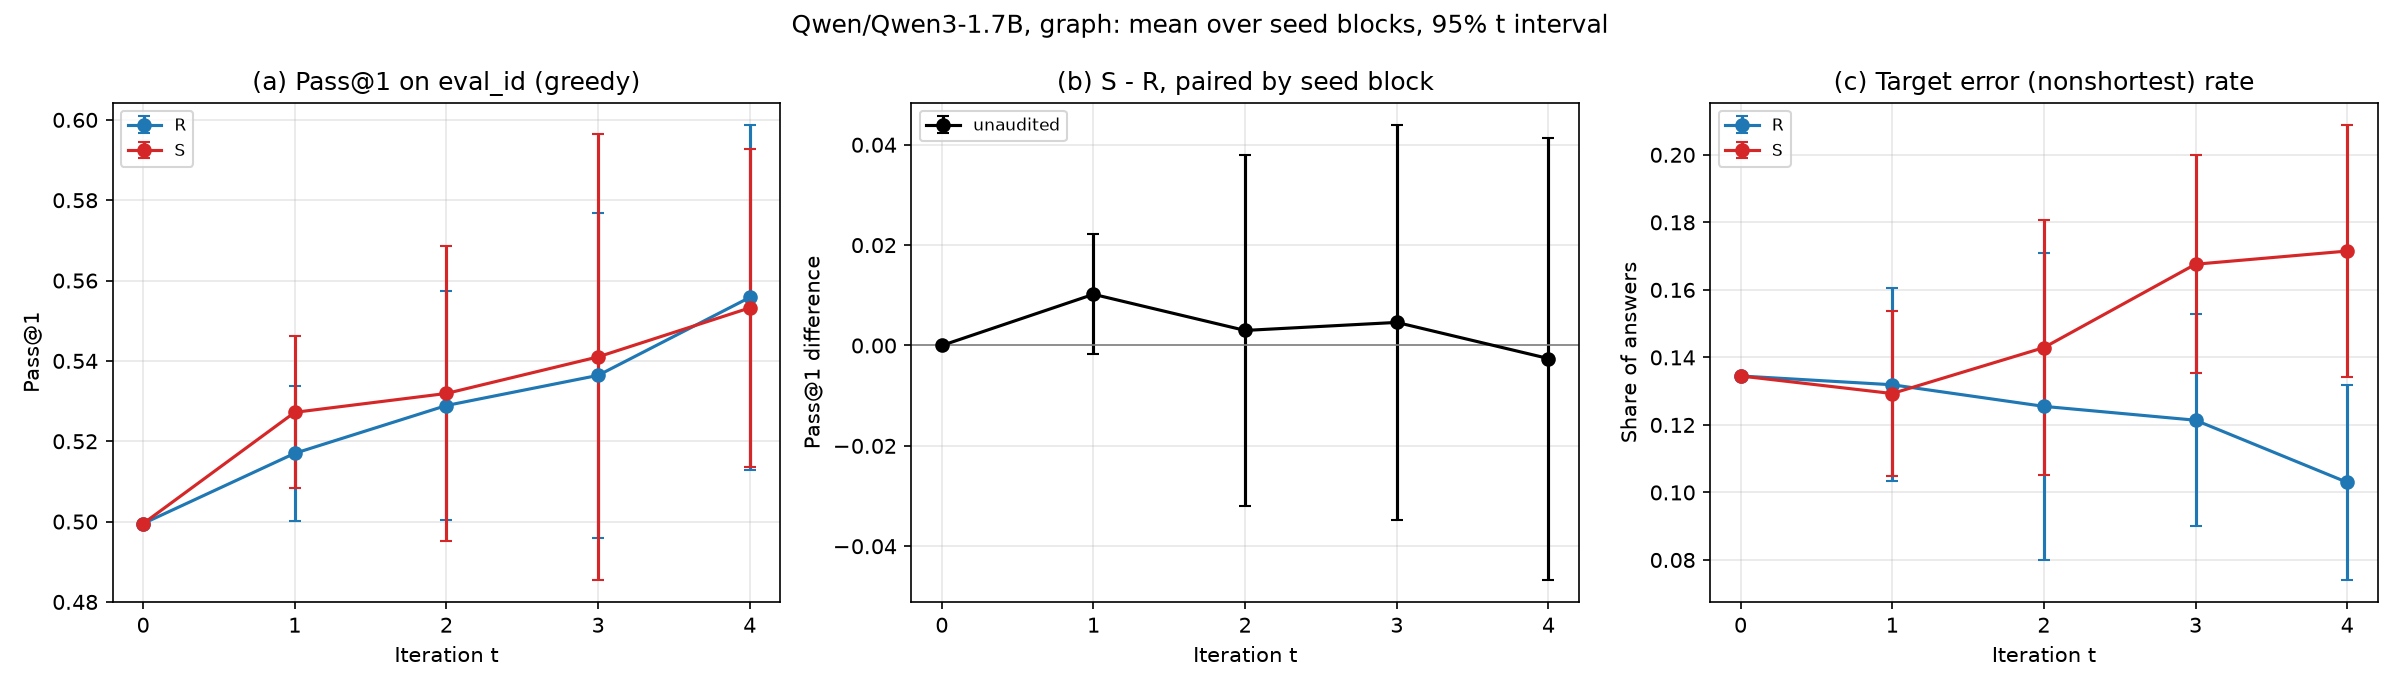
\includegraphics[width=0.90\linewidth]{figures/qwen_four_round_raw/unaudited_eval_id_pass1.png}
\par\smallskip
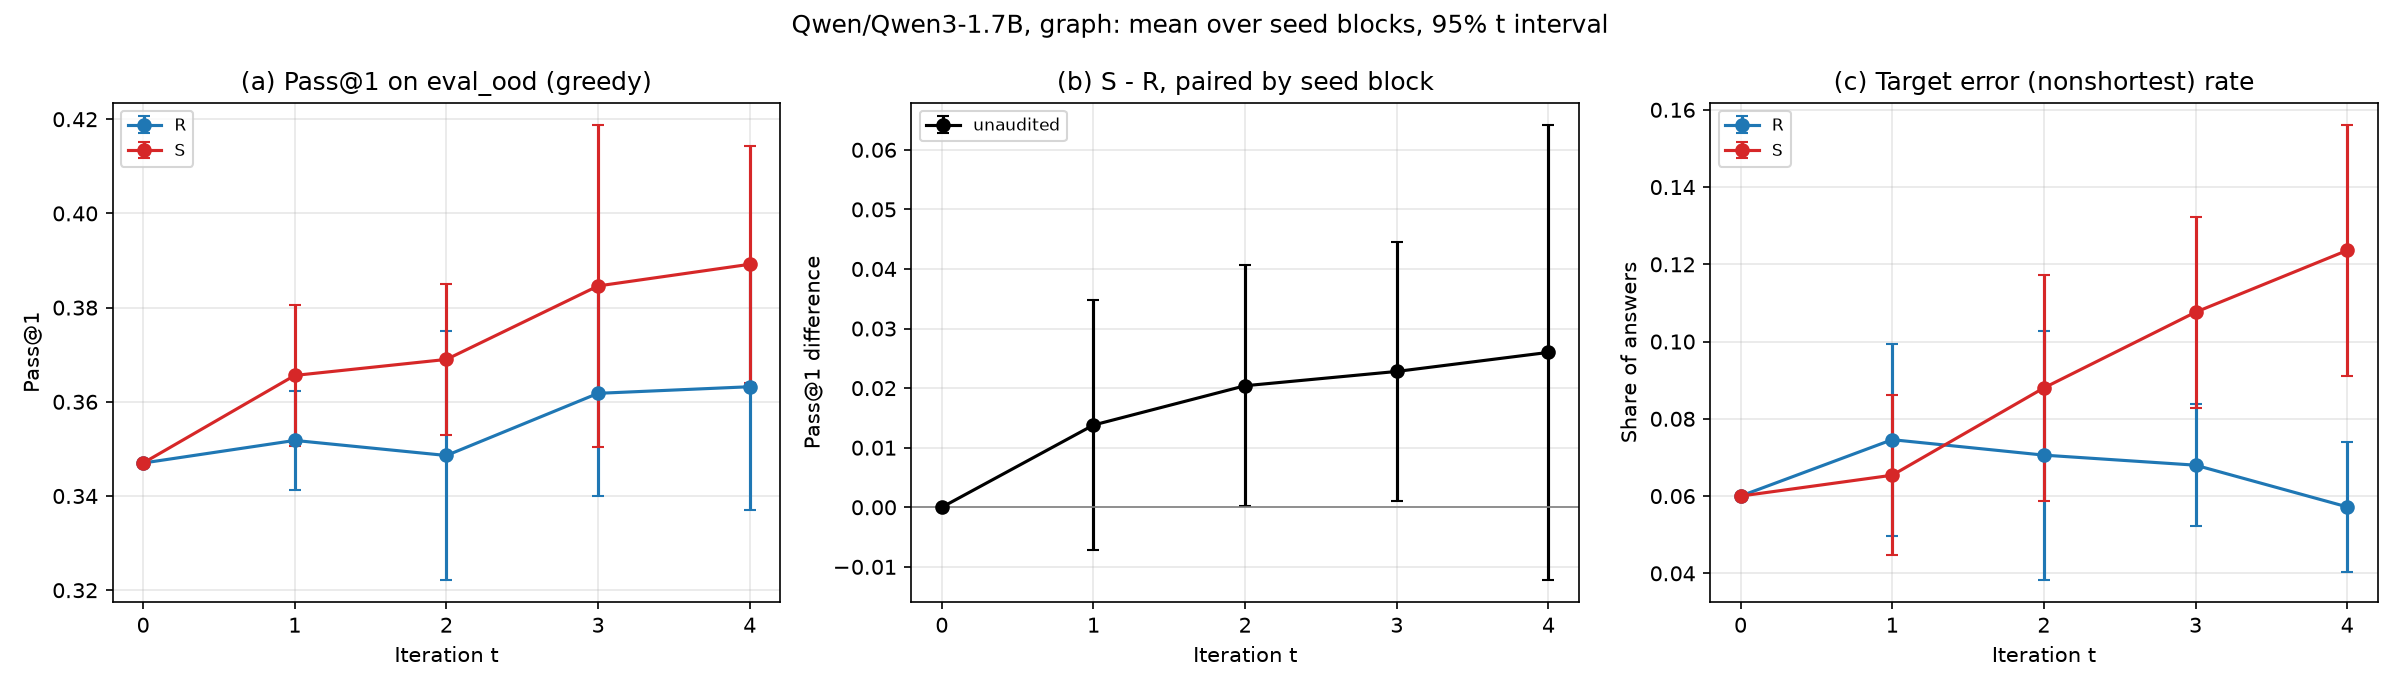
\includegraphics[width=0.90\linewidth]{figures/qwen_four_round_raw/unaudited_eval_ood_pass1.png}
\caption{Original unaudited Qwen3-1.7B graph curves, ID (top) and OOD
(bottom), for rounds 0--4. The three panels show greedy Pass@1, paired
$S-R$ accuracy, and nonshortest-error incidence among all answers.}
\label{fig:qwen-raw-unaudited}
\end{figure}

The unaudited arms reach round-four accuracy $0.556/0.553$ ID and
$0.363/0.389$ OOD, up from the common bases $0.4995$ and $0.3470$.
Nonshortest-error contrasts are $0.068\pm0.039$ ID and
$0.066\pm0.038$ OOD. Thus similar aggregate accuracy can coexist
with a difference in the composition of incorrect answers.

\begin{figure}[H]
\centering
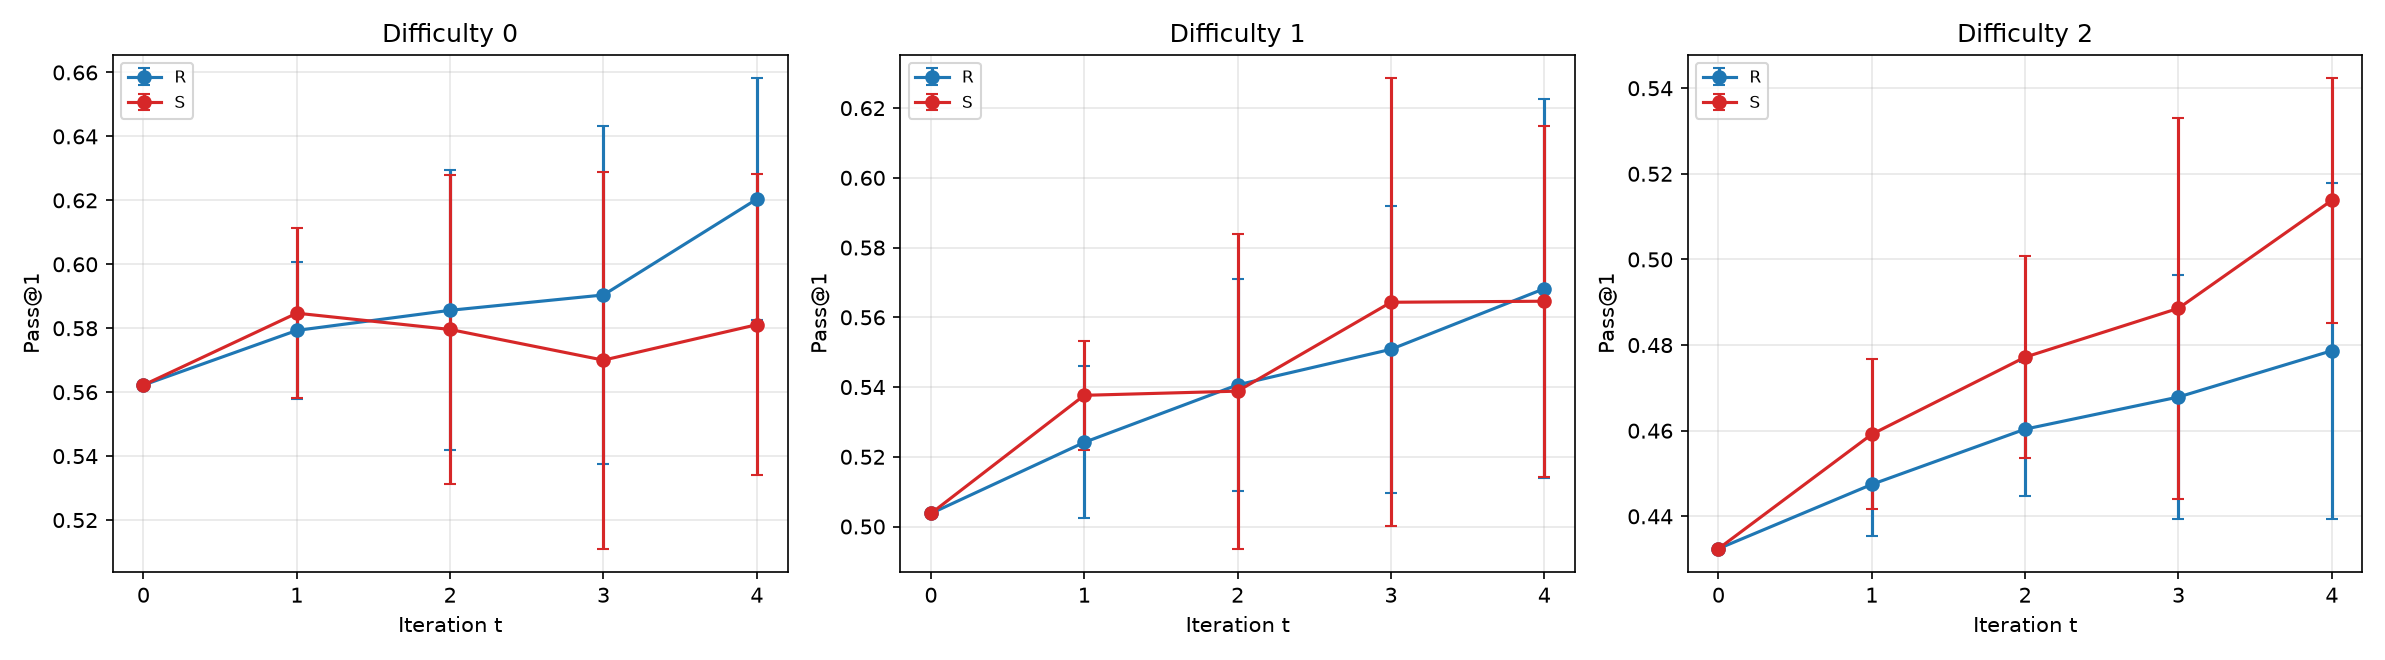
\includegraphics[width=0.90\linewidth]{figures/qwen_four_round_raw/unaudited_eval_id_by_difficulty.png}
\par\smallskip
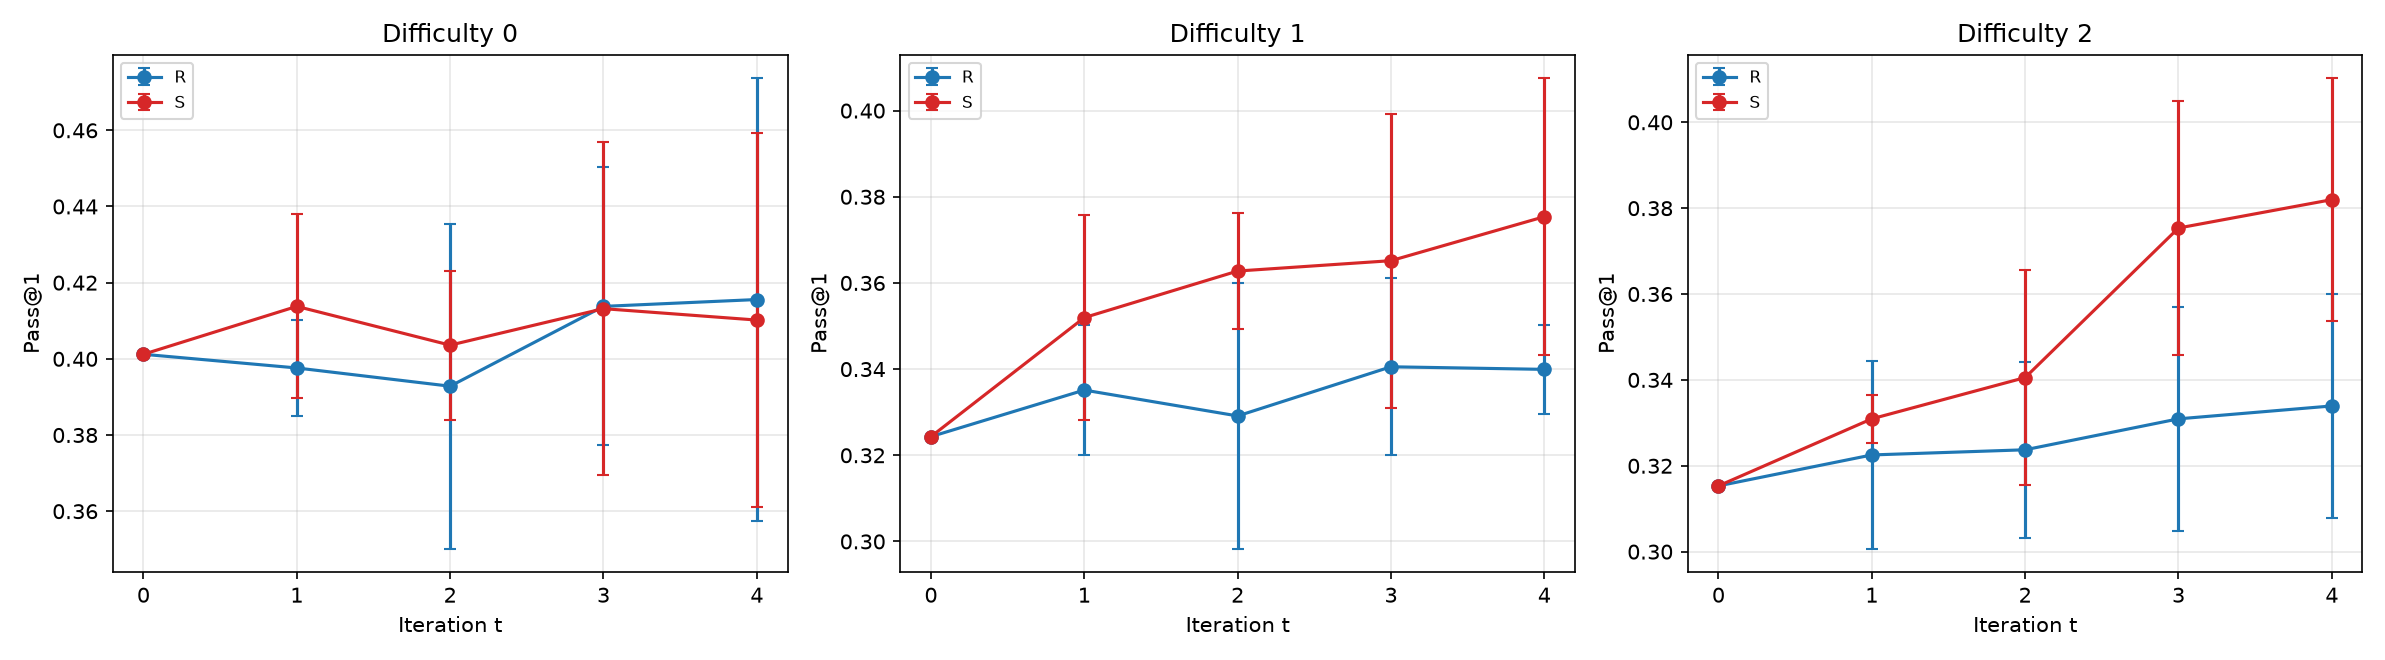
\includegraphics[width=0.90\linewidth]{figures/qwen_four_round_raw/unaudited_eval_ood_by_difficulty.png}
\caption{Original unaudited Qwen3-1.7B graph accuracy by generator
difficulty stratum, ID (top) and OOD (bottom), for rounds 0--4.
Strata 0--2 run from left to right and contain $667/667/666$ ID
and $334/333/333$ OOD questions. Error bars use the same five blocks
as Figure~\ref{fig:qwen-raw-unaudited}.}
\label{fig:qwen-raw-unaudited-difficulty}
\end{figure}

The strata are fixed features of the task generator, not an empirically
established ordering of model difficulty. Their separate vertical scales
are retained, so visual differences in slope do not by themselves
establish different learning rates. These descriptive trajectories
support no additional difficulty-specific significance claim.

\begin{figure}[H]
\centering
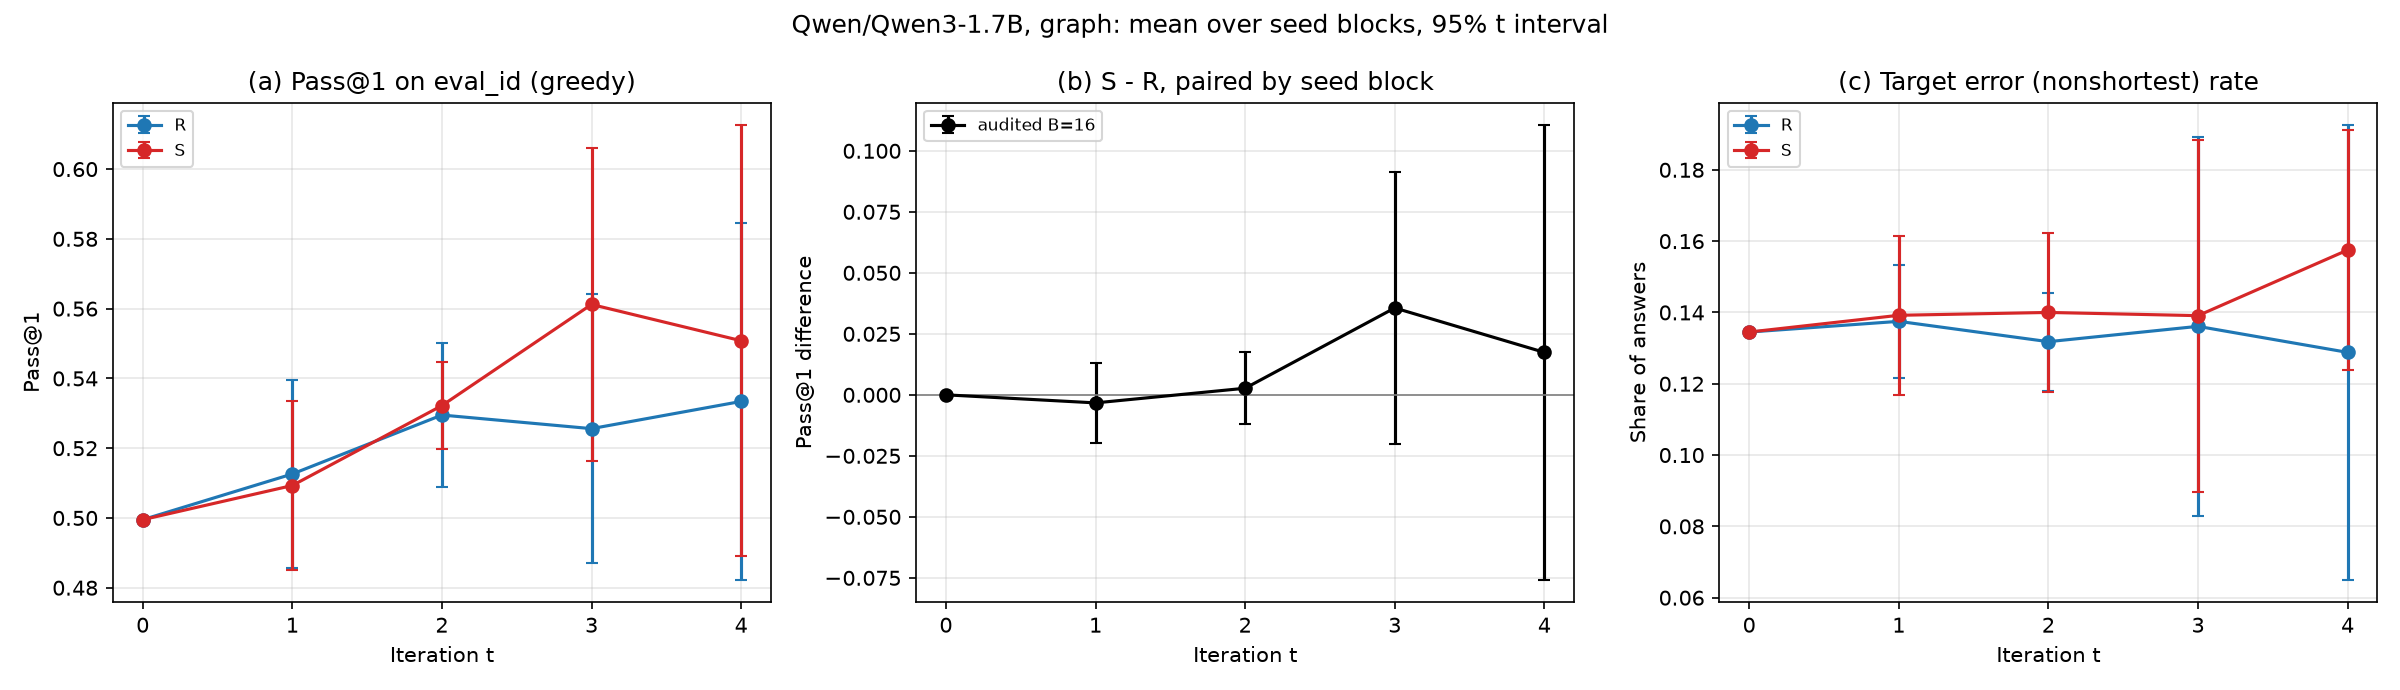
\includegraphics[width=0.90\linewidth]{figures/qwen_four_round_raw/audited_eval_id_pass1.png}
\par\smallskip
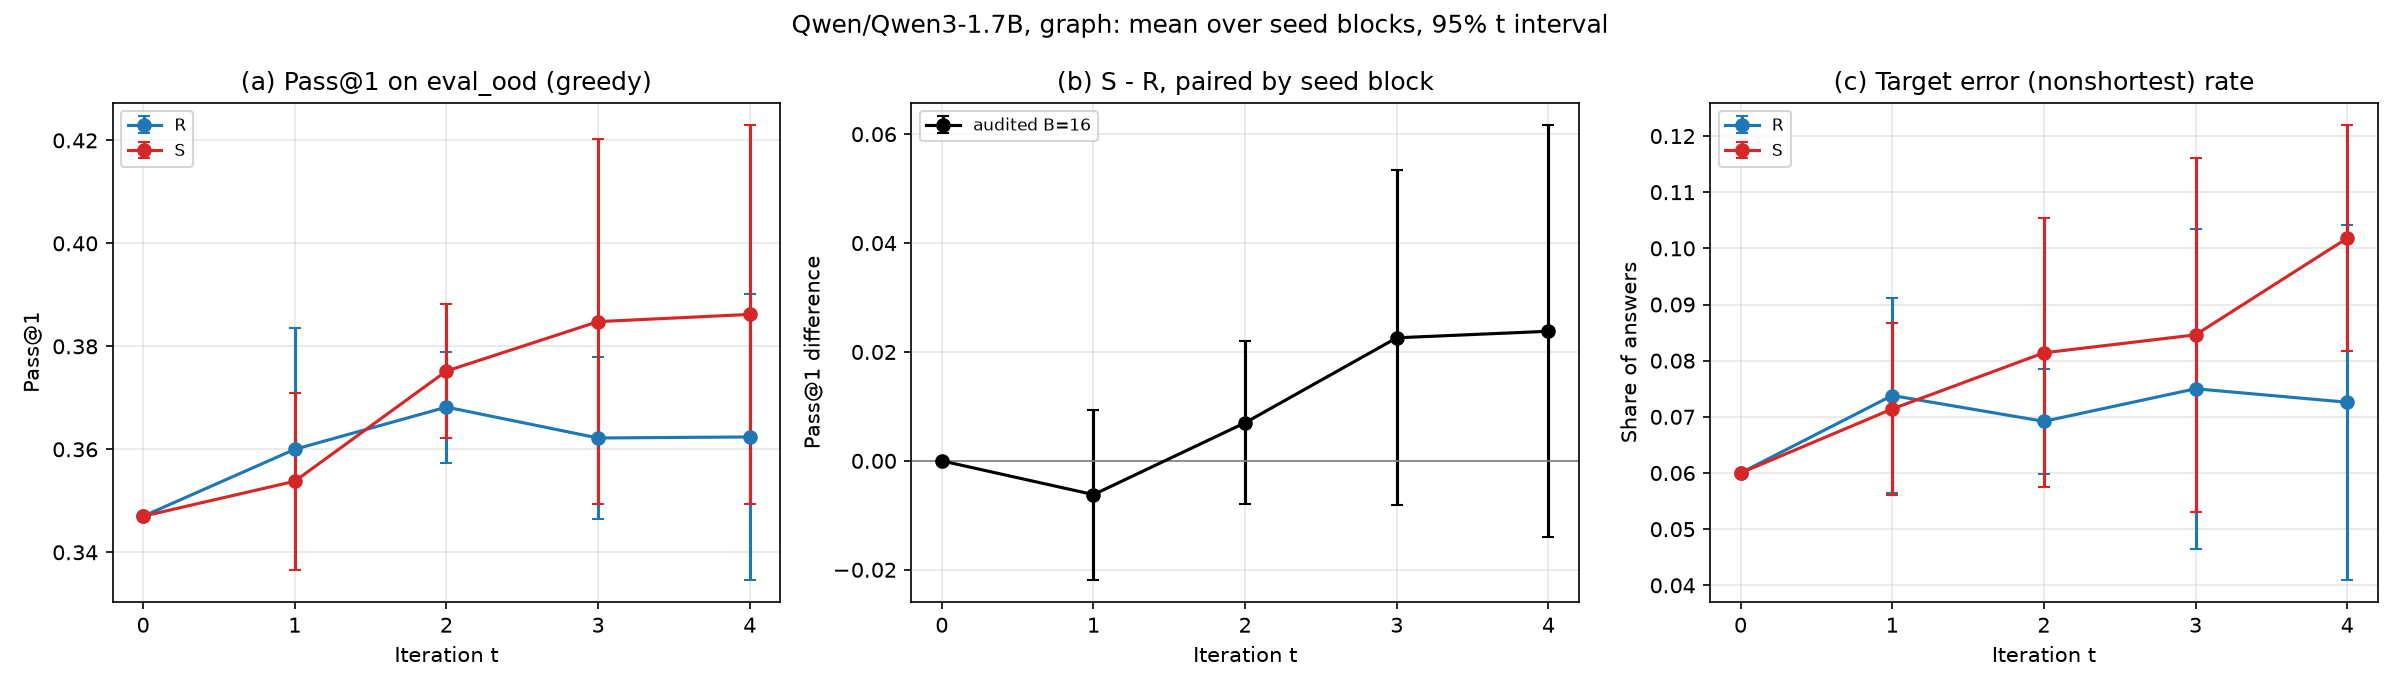
\includegraphics[width=0.90\linewidth]{figures/qwen_four_round_raw/audited_eval_ood_pass1.png}
\caption{Original adaptive-audit Qwen3-1.7B graph curves, ID (top)
and OOD (bottom), with $B_{\rm qry}=16$ correctness queries per
arm-round. The panels show greedy Pass@1, paired $S-R$ accuracy,
and nonshortest-error incidence. Each audited arm spends 64 queries
over four rounds.}
\label{fig:qwen-raw-audited}
\end{figure}

Under auditing, round-four $R/S$ accuracy is $0.533/0.551$ ID and
$0.362/0.386$ OOD. The paired contrasts are $0.017\pm0.093$ and
$0.024\pm0.038$, respectively. These contrasts
compare selection arms within the audited policy; they do not measure
the effect of adding an audit to an otherwise fixed training procedure.

\begin{figure}[H]
\centering
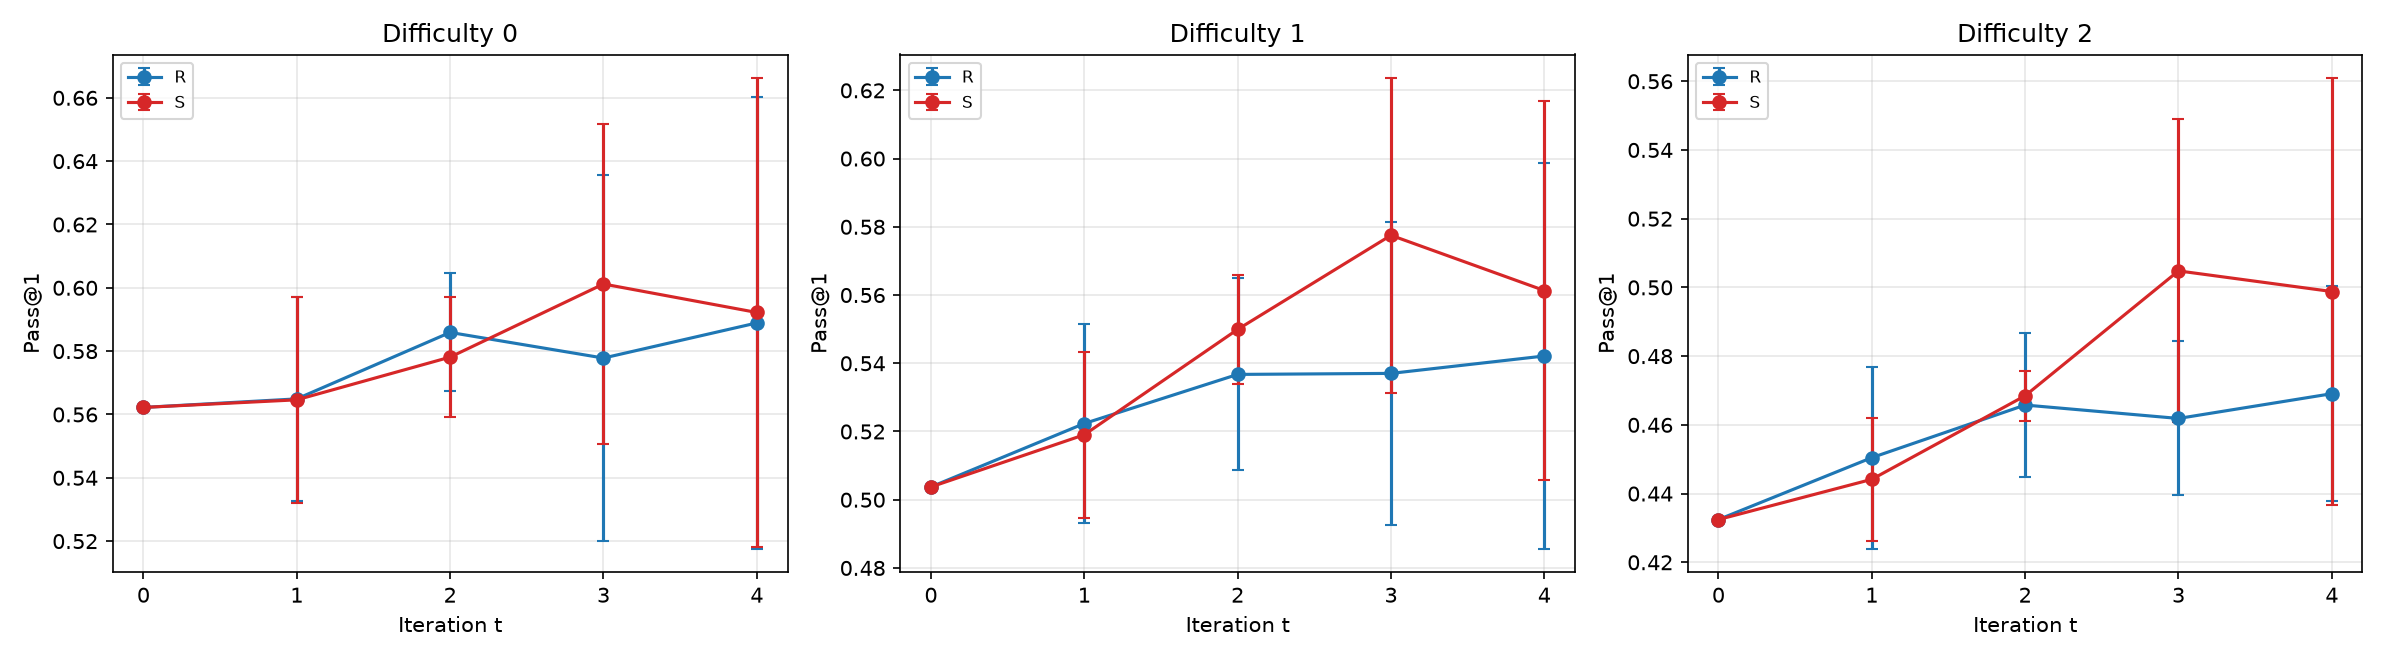
\includegraphics[width=0.90\linewidth]{figures/qwen_four_round_raw/audited_eval_id_by_difficulty.png}
\par\smallskip
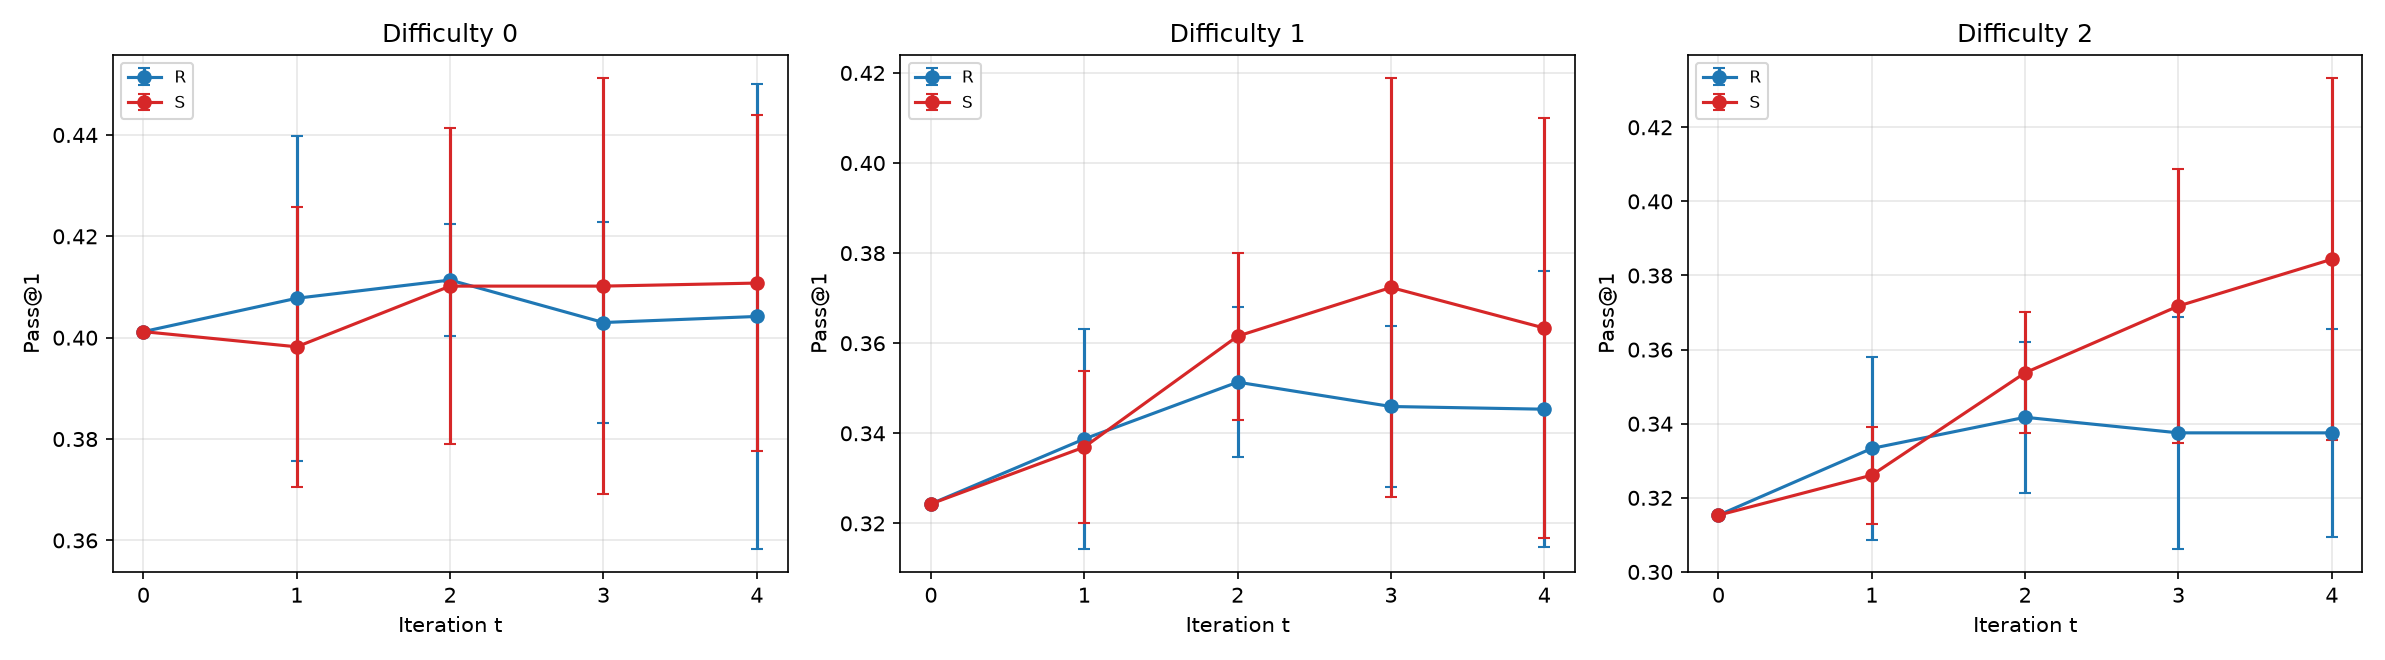
\includegraphics[width=0.90\linewidth]{figures/qwen_four_round_raw/audited_eval_ood_by_difficulty.png}
\caption{Original adaptive-audit Qwen3-1.7B graph accuracy by
generator stratum, ID (top) and OOD (bottom), for rounds 0--4.
The strata, fixed question sets, and pointwise block-$t$ intervals
follow Figure~\ref{fig:qwen-raw-unaudited-difficulty}.}
\label{fig:qwen-raw-audited-difficulty}
\end{figure}

The audited stratum curves supplement the aggregate results but do not
establish a stratum-specific audit benefit. They use the same fixed
questions as the unaudited curves, while retaining their original
separate vertical scales and pointwise uncertainty intervals.

\begin{figure}[H]
\centering
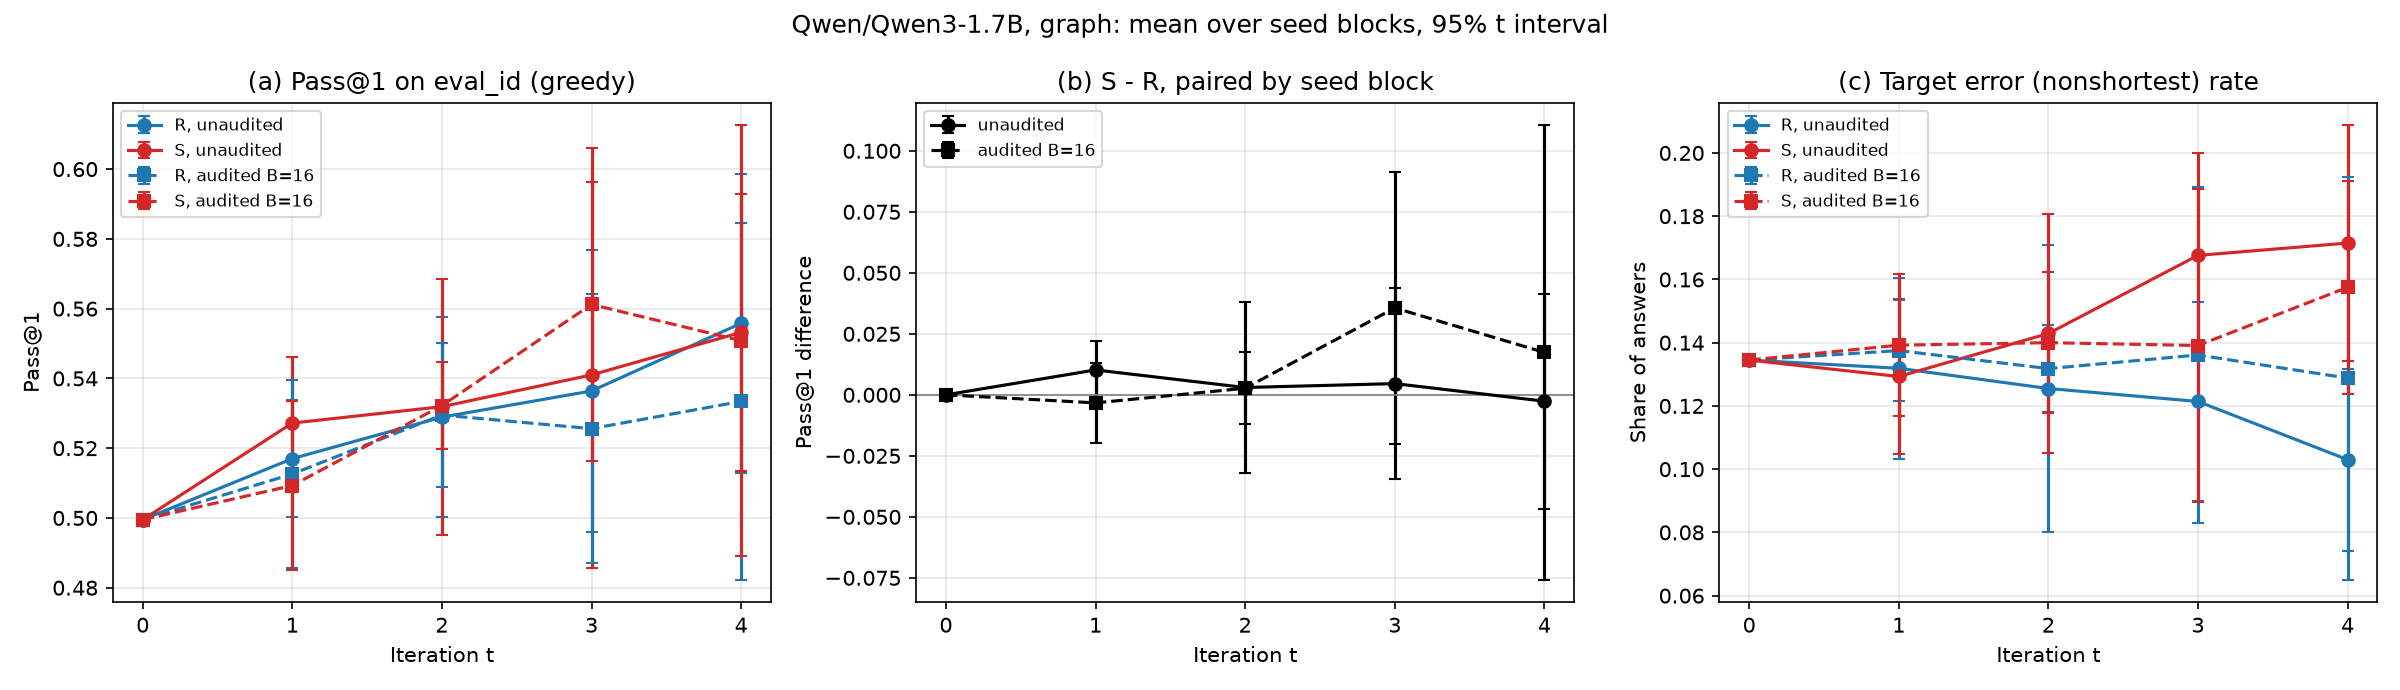
\includegraphics[width=0.90\linewidth]{figures/qwen_four_round_raw/comparison_eval_id_pass1.png}
\par\smallskip
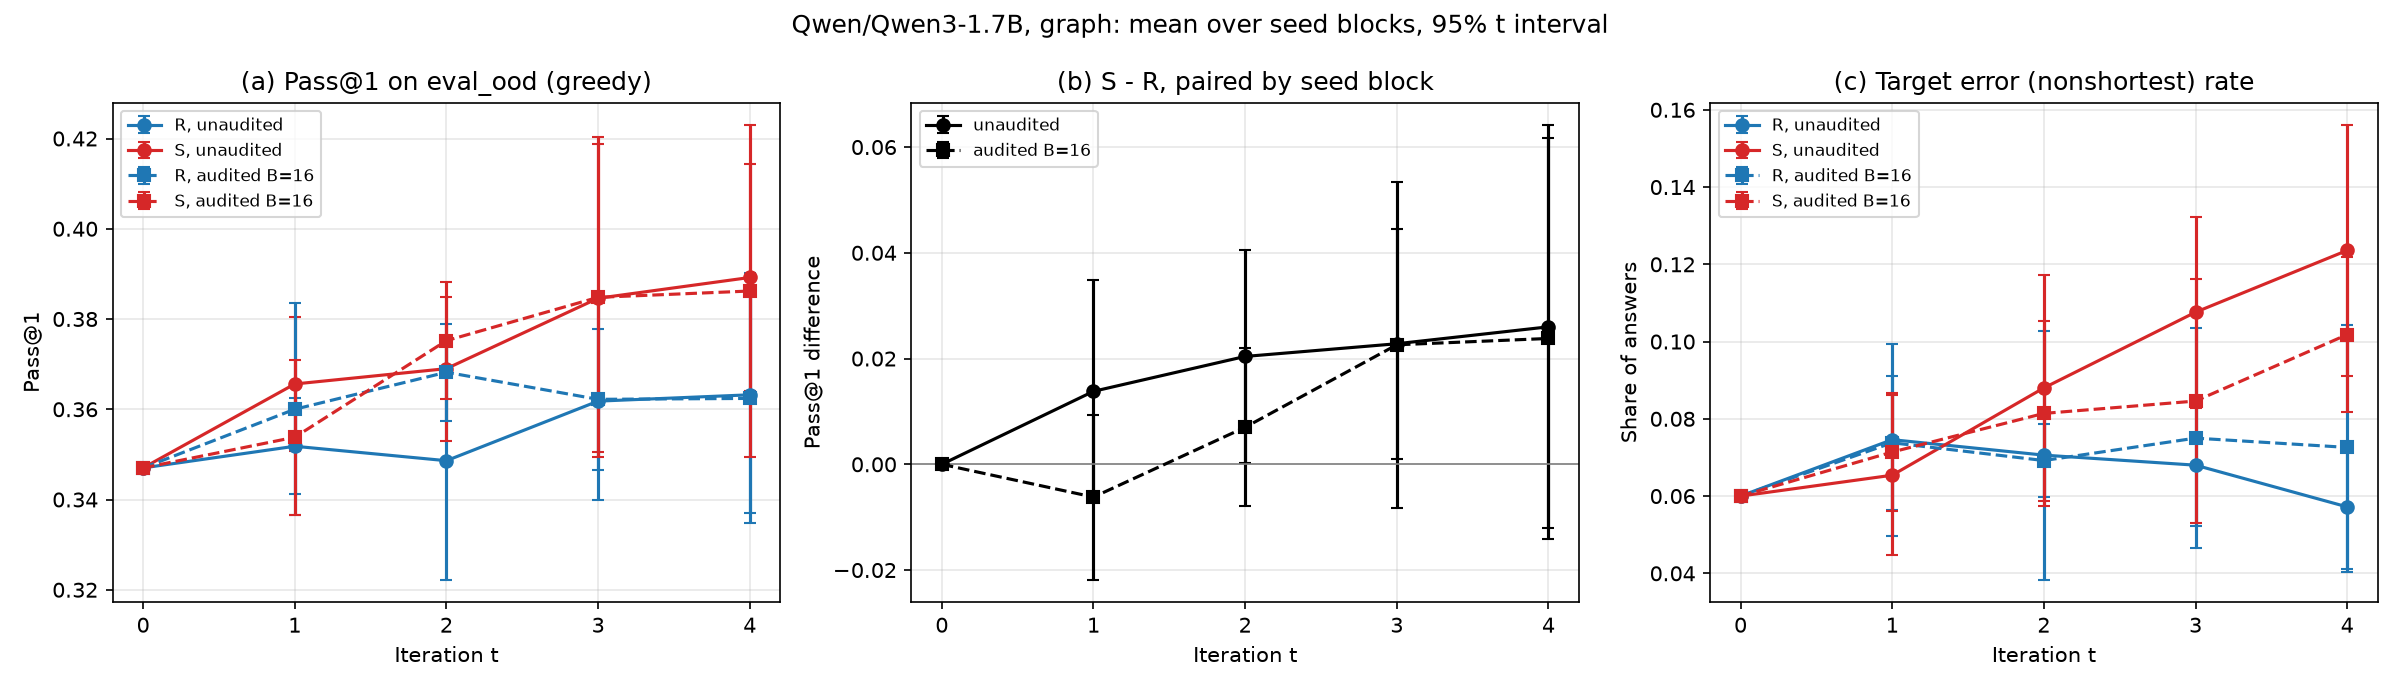
\includegraphics[width=0.90\linewidth]{figures/qwen_four_round_raw/comparison_eval_ood_pass1.png}
\caption{Original joint comparison of unaudited and adaptive-audit
Qwen3-1.7B graph trajectories, ID (top) and OOD (bottom), for
rounds 0--4. Each middle panel reports paired $S-R$ accuracy
separately within the two policies, not the effect of auditing.}
\label{fig:qwen-raw-comparison}
\end{figure}

Same-arm audited-minus-unaudited accuracy changes are negative in mean
(Table~\ref{tab:qwen-audit-change}).
The joint view therefore does not establish a uniform audit benefit;
it distinguishes within-policy arm differences from cross-policy changes.

\begin{figure}[H]
\centering
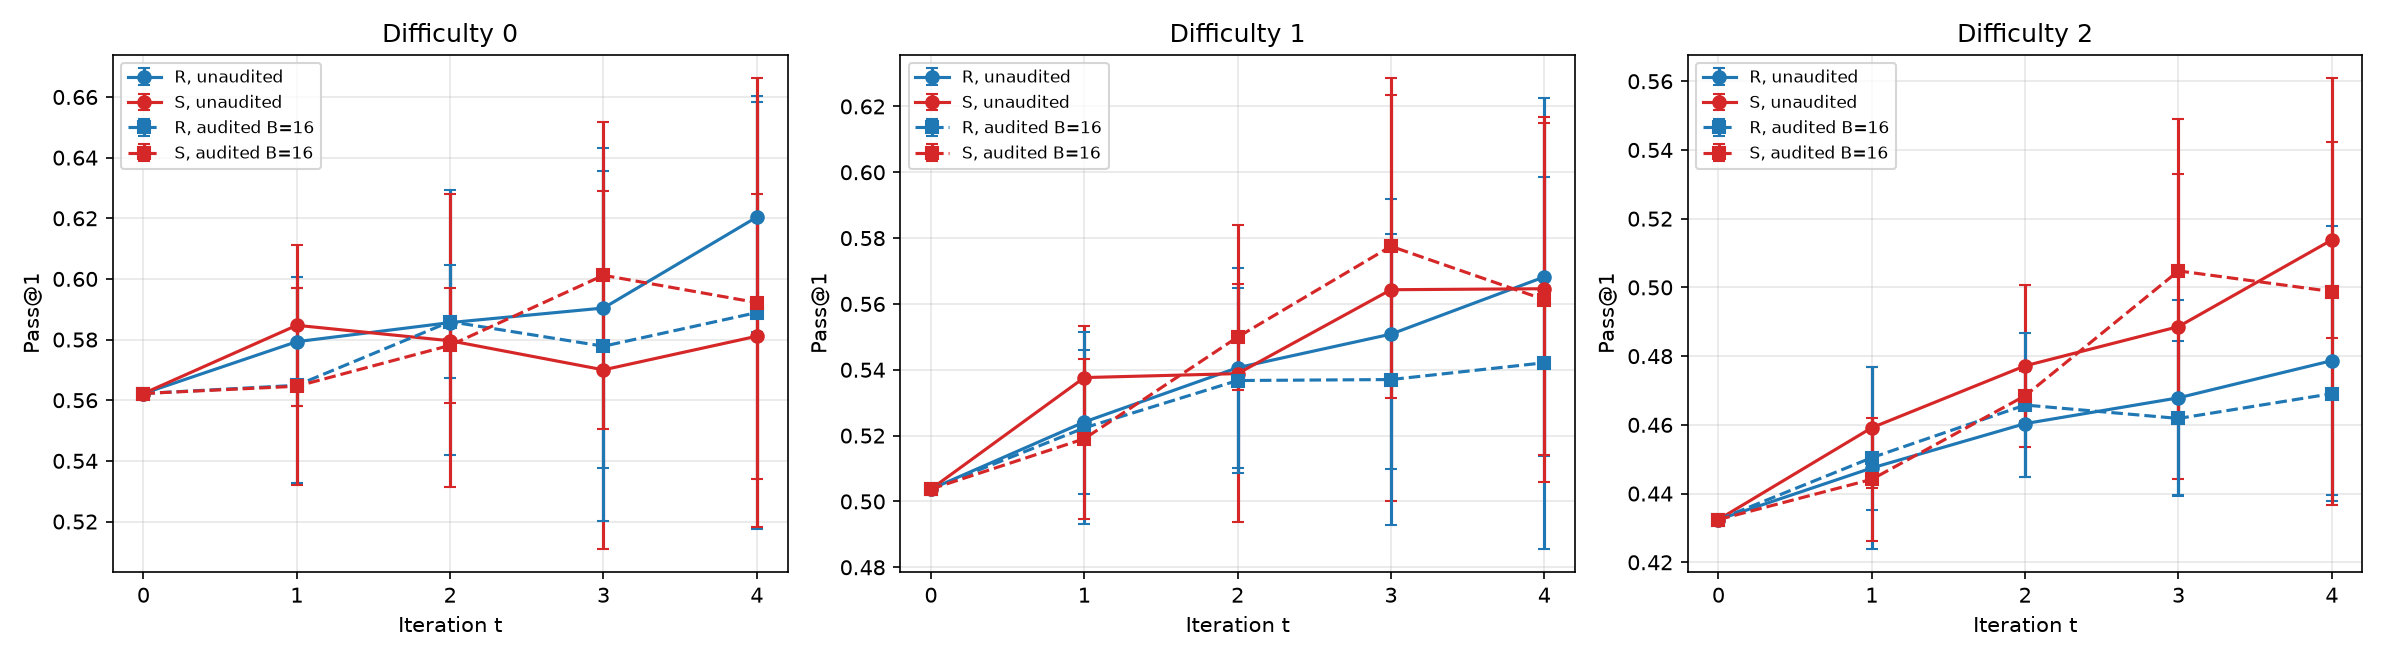
\includegraphics[width=0.90\linewidth]{figures/qwen_four_round_raw/comparison_eval_id_by_difficulty.png}
\par\smallskip
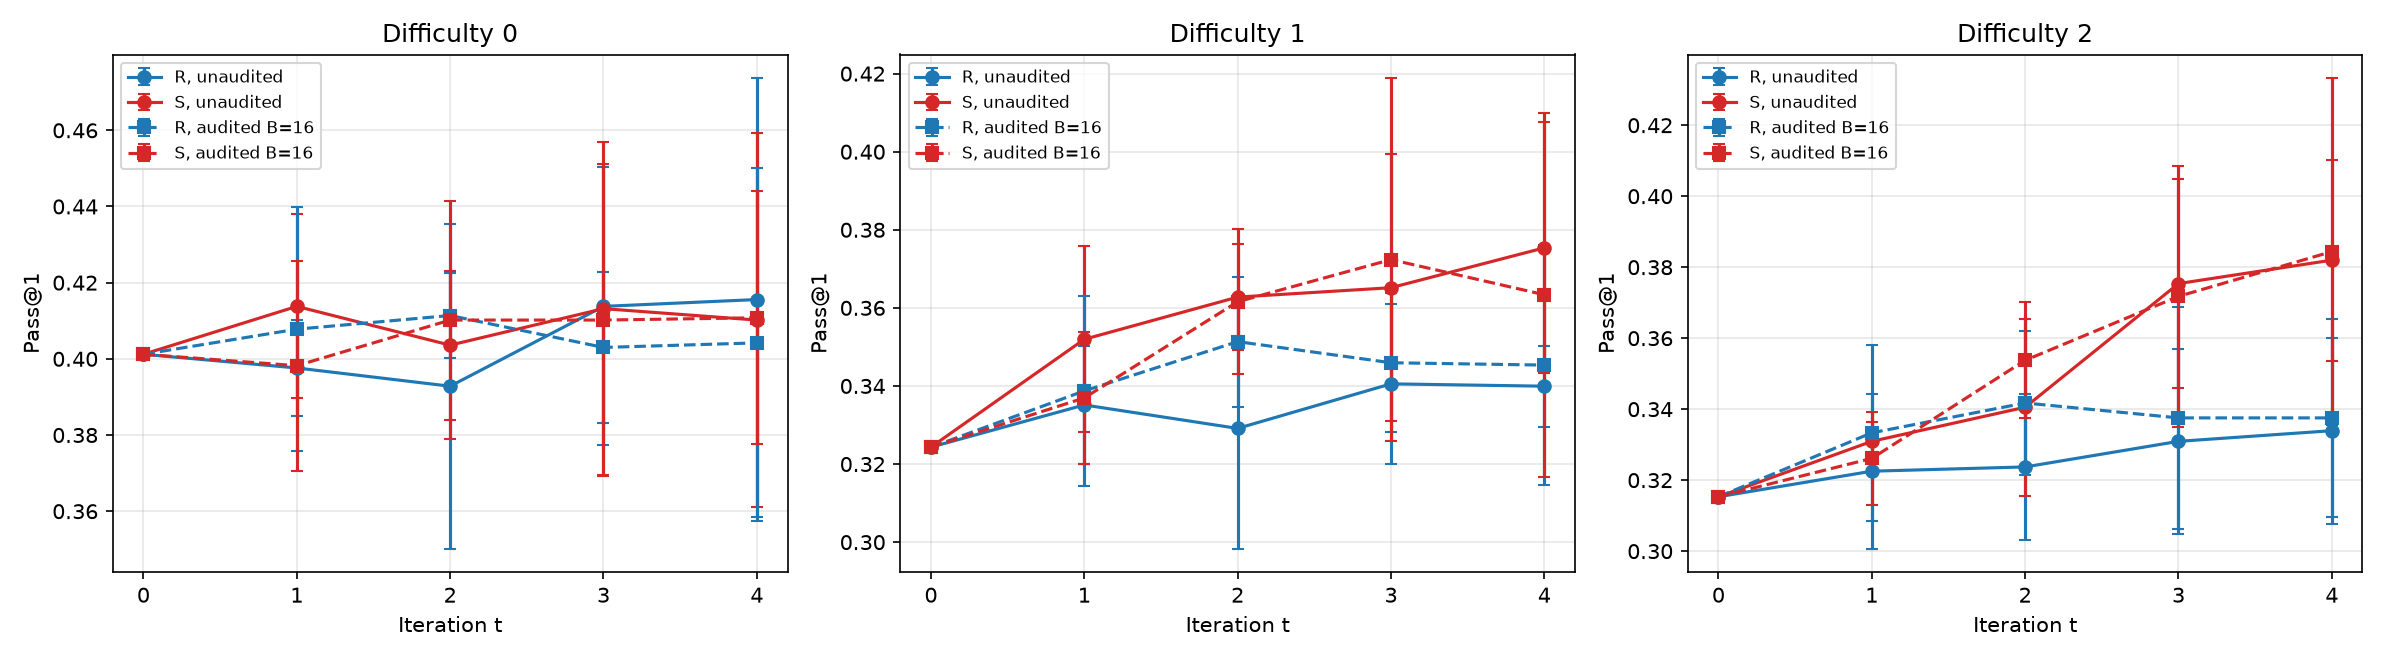
\includegraphics[width=0.90\linewidth]{figures/qwen_four_round_raw/comparison_eval_ood_by_difficulty.png}
\caption{Original joint Qwen3-1.7B graph accuracy curves by
generator stratum, ID (top) and OOD (bottom), for rounds 0--4.
Both policies and both arms use the same question stratum at
each checkpoint. Counts and interval conventions follow
Figure~\ref{fig:qwen-raw-unaudited-difficulty}.}
\label{fig:qwen-raw-comparison-difficulty}
\end{figure}

Both policies and both arms are evaluated on the same question stratum
at each checkpoint. Panel-specific vertical scales remain unchanged,
and the intervals are not adjusted for comparisons across strata,
rounds, or policies. The joint breakdown is consequently descriptive,
rather than a collection of confirmatory stratum-level tests.
\endgroup


\paragraph{Eight-round extension.}
The Llama-3.2-3B and Qwen3-1.7B trajectories continue to eight rounds.
Table~\ref{tab:eight-round-contrasts} reports the later paired accuracy
contrasts while retaining round four as the primary endpoint.
The unaudited Qwen3-1.7B OOD contrast favors $S$; these secondary
comparisons are descriptive and are not adjusted for multiplicity.
\begin{table}[H]
\caption{Round-eight graph accuracy contrasts $S-R$ (mean $\pm$ descriptive 95\% paired block-$t$ half-width over five blocks). Positive values favor $S$. ID and OOD evaluations use 2,000 and 1,000 fixed questions, respectively. These secondary endpoints supplement the primary four-round analysis.}
\label{tab:eight-round-contrasts}
\centering\small
\begin{tabular}{@{}llcc@{}}
\toprule
Model & Policy & ID Pass@1 $S-R$ & OOD Pass@1 $S-R$\\
\midrule
Llama-3.2-3B & Unaudited & $-0.029\pm0.111$ & $0.024\pm0.064$\\
Llama-3.2-3B & Adaptive, $B=16$ & $-0.031\pm0.086$ & $0.015\pm0.081$\\
Qwen3-1.7B & Unaudited & $0.040\pm0.045$ & $0.047\pm0.042$\\
Qwen3-1.7B & Adaptive, $B=16$ & $0.029\pm0.091$ & $0.037\pm0.063$\\
\bottomrule
\end{tabular}
\end{table}


\subsection{Qwen3-4B: four-round graph comparisons}
\label{app:qwen4b-four-round}

Both Qwen3-4B policies comprise five paired blocks and four rounds,
evaluated greedily on 2,000 ID and 1,000 OOD questions.
Table~\ref{tab:qwen4b-endpoints} reports endpoint accuracy and target incidence.
Unaudited OOD accuracy contrasts
at rounds two and three are $0.0308\pm0.0243$ and $0.0388\pm0.0233$,
but this intermediate advantage does not persist at round four.
These comparisons are not adjusted for multiplicity and do not constitute
a best-checkpoint analysis.

\input{qwen4b_matching_table}
\input{qwen4b_multiround_endpoint_table}

The identical round-one certificates confirm shared prompt/correct-response IDs,
$48/16$ correct/error counts, and exact response-token matching.
$R$ selects 9--10 nonshortest errors, versus 16 in $S$.
Audited training rows and weights agree with the reported
selection counts and effective sample sizes. Later pools are not jointly rate-matched.
Generation uses temperature $1.3$, top-$p=1$, and a mixed stopping schedule: block
\texttt{b00} uses no repetition stop throughout; \texttt{b01} introduces
it at round four, and \texttt{b02}--\texttt{b04} use it in later-round
generation throughout. The two arms share each block-round setting.
Their imported round-one pools were generated without this stop rule.
Thus the study is not a replication under one uniform generation profile.

Both policies improve in mean.
Same-arm audit error changes are positive in mean
(Table~\ref{tab:audit-results}). Each audited arm spends 64
queries per block, averaging 54.4/55.0 $R/S$ updates versus 64 unaudited.
These descriptive contrasts combine changes in data, weighting,
and optimizer effort.

Tables~\ref{tab:qwen4b-rounds} and~\ref{tab:qwen4b-blocks} report all four
rounds and all five endpoint blocks, rather than a selected checkpoint.
Table~\ref{tab:qwen4b-audit-change} gives accuracy changes with their
paired intervals, complementing the error changes in
Table~\ref{tab:audit-results}. Table~\ref{tab:qwen4b-audit} reports each
round's projection, retained volume, positive-weight coverage, ESS, and
TPRs. Retained-row TPR equals pre-audit TPR because audit deletion
preserves all 48 correct rows; positive-weight TPR can be smaller.
Rates use each round's original nontruncated-pool denominator and are
averages of block-level ratios, not ratios of pooled counts.
Table~\ref{tab:qwen4b-training} complements these readouts with per-round
parameter-change norms and training losses for the completed comparisons.
These quantities describe the training objective, not held-out accuracy;
losses under different weighting policies are not directly comparable.

\input{qwen4b_trajectory_table}
\input{qwen4b_blocks_table}
\input{qwen4b_audit_contrast_table}
\input{qwen4b_audit_readouts_table}
\input{qwen4b_training_table}

\paragraph{Validation scope.}
Accuracy and target incidence are reconstructed from 82 checkpoint--split
count records per policy, with all 40 training completions per policy checked.
All 123,000 audited held-out responses are independently rejudged, including
truncated answers in the evaluation denominators. Audit queries, retained
volume, positive-weight counts, and ESS agree with the training records.
Unaudited validation remains count-based because answers are unavailable.
Audited checkpoints are not reloaded; missing shared initialization and
reference tensors preclude independent gradient recomputation.
The 81,920 shared round-one candidate responses are also independently
rejudged; eligible-pool counts agree with the matching certificates.
Exact-length eligibility is reported from those certificates rather than
independently retokenized.

\begin{figure}[H]
\centering
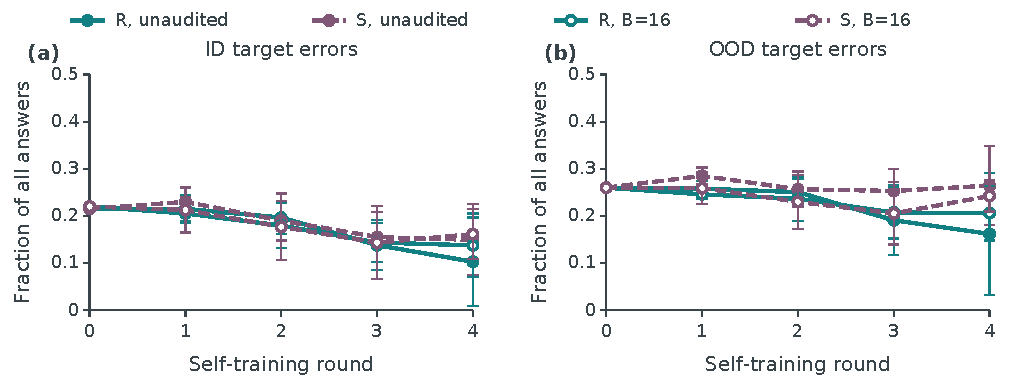
\includegraphics[width=0.8\linewidth]{figures/qwen4b_multiround/qwen4b_target_errors.pdf}
\caption{Qwen3-4B nonshortest-error incidence among all evaluated answers.
Unaudited $R/S$ endpoints are $0.1026/0.1491$ ID and $0.1618/0.2644$ OOD;
audited endpoints are $0.1375/0.1614$ and $0.2060/0.2424$.
Paired contrasts appear in Table~\ref{tab:qwen4b-endpoints}.
Bars are pointwise block-$t$ intervals
over five blocks.}
\label{fig:qwen4b-target-errors}
\end{figure}

\input{qwen4b_four_round_raw_figures}


\subsection{Completed isolated one-step graph comparisons}
\label{app:one-step-results}

The isolated one-step graph studies are complete for Qwen3-1.7B,
Qwen3-4B, and Llama-3.2-3B-Instruct. Each uses five blocks, the original
matched round-one $K=64$ subsets, and one full-batch AdamW update per
$R/S$ arm at learning rate $5\times10^{-5}$, zero weight decay,
clipping threshold 1, and the same rank-8, $\alpha=16$, zero-dropout
\texttt{q\_proj}/\texttt{v\_proj} LoRA configuration. A dedicated
64-example reference gradient is bound to this configuration and initial
adapter; no multiround reference gradient is substituted. The null takes
zero updates and has exactly zero displacement and projection.
Table~\ref{tab:one-step-heldout} therefore reports measured one-step
outcomes, not first-round multistep results.

Table~\ref{tab:risk} brings together the one-step outcomes and update
diagnostics.
\begin{table}[H]
\caption{Unaudited one-step matrix. The three graph comparisons are complete: five paired blocks each, one AdamW update per $R/S$ arm, and an un-updated shared null. Separate rows identify the two arms. The primary paired contrast is $S-R$ in ID greedy Pass@1 (positive favors $S$), with a descriptive 95\% block-$t$ half-width, reported on the $S$ row. Multiround checkpoints are not substituted.}
\label{tab:risk}
\centering\small\setlength{\tabcolsep}{3pt}
\begin{tabular}{@{}lllcccccc@{}}
\toprule
Model & Task & Blocks & Arm & ID error & OOD error & \shortstack{ID Pass@1\\$S-R$} & $h^T\Delta\theta$ & $\|\Delta\theta\|_2$\\
\midrule
Qwen3-1.7B & Graph & 5 & $R$ & 0.4972 & 0.6470 & & $-0.00504$ & 0.0414\\
 & & & $S$ & 0.4970 & 0.6472 & $0.0002\pm0.0009$ & $-0.00540$ & 0.0414\\
\addlinespace
Qwen3-4B & Graph & 5 & $R$ & 0.3890 & 0.6040 & & $-0.00689$ & 0.0605\\
 & & & $S$ & 0.3896 & 0.6018 & $-0.0006\pm0.0036$ & $-0.00804$ & 0.0606\\
\addlinespace
Llama-3.2-3B & Graph & 5 & $R$ & 0.7502 & 0.7848 & & $-0.01850$ & 0.0478\\
 & & & $S$ & 0.7493 & 0.7838 & $0.0009\pm0.0028$ & $-0.01847$ & 0.0478\\
\addlinespace
Llama-3.2-3B & Arithmetic & 5 & --- & \TBD & \TBD & \TBD & \TBD & \TBD\\
Llama-3.2-1B & Arithmetic & 5 & --- & \TBD & \TBD & \TBD & \TBD & \TBD\\
\bottomrule
\end{tabular}
\end{table}


Protocol validation confirms complete evaluation of all eleven checkpoints
per split. Our analysis independently checks the available
training IDs, unit weights, 48/16 diagnostic label counts, matching
certificates, step counts, scalar diagnostic consistency, and held-out
count identities. It reproduces the supplied plot means, SDs and
paired intervals. Saved gradient-composition residuals are below the
recorded tolerance, but this scalar-record check does not reconstruct
the unavailable gradient or adapter tensors. Original execution checks
verified adapter identity; independent tensor-level verification requires
the unavailable adapters.

The Qwen3-1.7B comparison reuses its four-round study's initial inputs.
Qwen3-4B uses candidate pools generated without the repetition-stop rule;
matching and evaluation follow the specified one-step protocol. These
pools are not treated as newly sampled under a different stopping rule.
The one-step base accuracies are $0.4980/0.3530$ ID/OOD for Qwen3-1.7B,
$0.6145/0.3920$ for Qwen3-4B, and $0.2455/0.2070$ for Llama.
They differ slightly from the four-round baselines despite shared evaluation
question identities for the overlapping models. We use each run's own
null, not a baseline pooled across studies. Model-to-model differences
therefore do not constitute a controlled model-size comparison.

\begin{figure}[H]
\centering
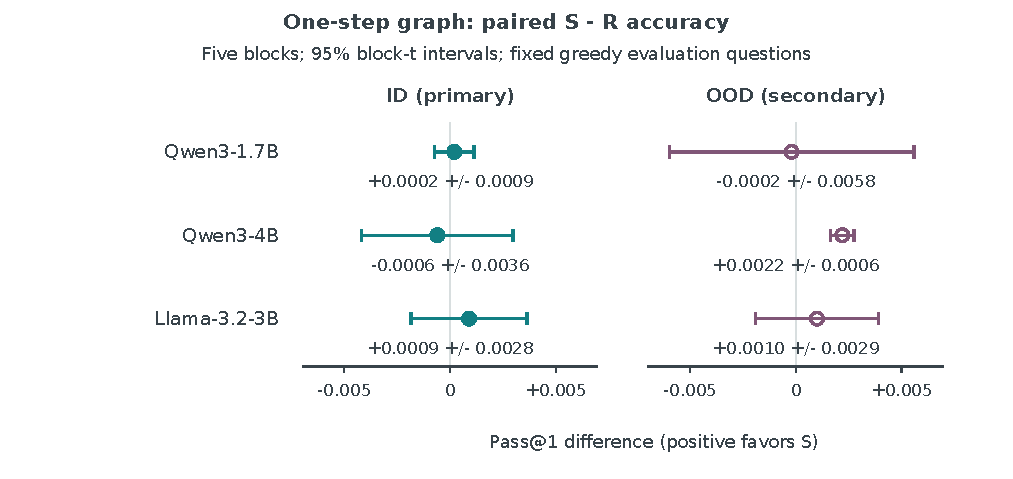
\includegraphics[width=0.85\linewidth]{figures/graph_extensions/one_step_contrasts.pdf}
\caption{Paired one-step graph accuracy contrasts $S-R$ in ID (primary)
and OOD (secondary), evaluated on each run's own fixed question sets.
Primary ID differences are $0.0002\pm0.0009$ for Qwen3-1.7B,
$-0.0006\pm0.0036$ for Qwen3-4B and $0.0009\pm0.0028$ for Llama.
Qwen3-4B's OOD difference is
$0.0022\pm0.0006$, with $S$ answering 2--3 more of the 1,000 OOD
questions correctly in every block. This secondary comparison is not
multiplicity-adjusted. Points and bars show means and descriptive 95\%
paired block-$t$ intervals over five blocks, not variation over model
initializations. Positive values favor $S$.}
\label{fig:one-step-contrasts}
\end{figure}

Relative to null, mean ID accuracy increases by
$0.0048/0.0050$ for Qwen3-1.7B $R/S$ and $0.0043/0.0052$ for Llama,
but decreases by $0.0035/0.0041$ for Qwen3-4B. Thus the common negative
mean reference projection is not a certificate of ID accuracy improvement.
For Qwen3-4B, the OOD advantage for $S$ is present in all five blocks;
the effect is small on the discrete question-count scale and remains a
secondary, unadjusted comparison.

Table~\ref{tab:one-step-diagnostics} decomposes the initial gradients
and reports actual displacement norms. Correct-gradient contributions
agree across arms, as expected from shared correct rows; the mean
error-gradient norm is larger in $S$ for all three models. This does not
alone determine an AdamW direction or prove that the targeted error
signature has higher reference-risk influence. Paired projection
contrasts are $-0.00035\pm0.00077$ (Qwen3-1.7B),
$-0.00115\pm0.00377$ (Qwen3-4B), and $0.00003\pm0.00063$ (Llama).
Both arms have negative projection in every
Qwen3-1.7B and Llama block; Qwen3-4B block \texttt{b00} has positive
projection in both arms. None of these pairs shows opposite projection
signs within a block.

Writing the LoRA correction as $(\alpha/r)BA$, the standard initialization
$B=0$ makes the initial gradient with respect to $A$ vanish.
For a fresh AdamW optimizer with zero weight
decay, bias correction gives the first update
$\Delta\theta=-\eta\,\widetilde g/(|\widetilde g|+\epsilon)$
coordinatewise, where $\widetilde g$ is the clipped gradient.
This is an ideal-arithmetic identity; it approximates a sign step only
when $|\widetilde g|\gg\epsilon$. Finite $\epsilon$ retains dependence
on gradient magnitude and clipping. The nearly equal $R/S$ displacement
norms therefore need not imply similar raw gradients.

\begin{table}[H]
\caption{One-step graph diagnostics at the shared initial adapter. $G_C$ and $G_E$ are correct/error contributions to the common full-batch gradient, not separately renormalized class means. Projections are surrogate first-order diagnostics, not certified reference-loss changes. Norms use measured AdamW displacements, not $-\eta G$. Clipping uses threshold 1.}
\label{tab:one-step-diagnostics}
\centering\small\setlength{\tabcolsep}{3pt}
\begin{tabular}{@{}llllllll@{}}
\toprule
Model & Arm & $h^T\Delta\theta$ & $\|\Delta\theta\|_2$ & $\|G_C\|_2$ & $\|G_E\|_2$ & $\|G\|_2$ & Clipped\\
\midrule
Qwen3-1.7B & R & $-0.00504\pm0.00217$ & 0.04139 & 0.8229 & 0.4366 & 0.9037 & 1/5\\
Qwen3-1.7B & S & $-0.00540\pm0.00230$ & 0.04139 & 0.8229 & 0.6204 & 0.9954 & 1/5\\
Qwen3-4B & R & $-0.00689\pm0.00969$ & 0.06054 & 0.4351 & 0.3051 & 0.5418 & 0/5\\
Qwen3-4B & S & $-0.00804\pm0.00722$ & 0.06055 & 0.4351 & 0.3186 & 0.5412 & 0/5\\
Llama-3.2-3B & R & $-0.01850\pm0.00244$ & 0.04782 & 0.5422 & 0.1847 & 0.6396 & 0/5\\
Llama-3.2-3B & S & $-0.01847\pm0.00261$ & 0.04782 & 0.5422 & 0.2030 & 0.6711 & 0/5\\
\bottomrule
\end{tabular}
\end{table}

\begin{table}[H]
\caption{Qwen3-1.7B one-step graph blocks. Each split uses the same fixed questions for its base/null and all ten trained checkpoints.}
\label{tab:one-step-blocks-graph_unaudited}
\centering\small\setlength{\tabcolsep}{3pt}
\begin{tabular}{@{}llllll@{}}
\toprule
Block & Arm & ID Pass@1 & OOD Pass@1 & $h^T\Delta\theta$ & $\|\Delta\theta\|_2$\\
\midrule
b00 & R & 0.5045 & 0.3530 & $-0.00589$ & 0.04138\\
b00 & S & 0.5040 & 0.3490 & $-0.00664$ & 0.04139\\
b01 & R & 0.5045 & 0.3560 & $-0.00515$ & 0.04139\\
b01 & S & 0.5045 & 0.3550 & $-0.00571$ & 0.04138\\
b02 & R & 0.5035 & 0.3520 & $-0.00467$ & 0.04140\\
b02 & S & 0.5030 & 0.3550 & $-0.00393$ & 0.04140\\
b03 & R & 0.5015 & 0.3550 & $-0.00712$ & 0.04138\\
b03 & S & 0.5025 & 0.3500 & $-0.00758$ & 0.04137\\
b04 & R & 0.5000 & 0.3490 & $-0.00238$ & 0.04138\\
b04 & S & 0.5010 & 0.3550 & $-0.00312$ & 0.04139\\
\bottomrule
\end{tabular}
\end{table}

\begin{table}[H]
\caption{Qwen3-4B one-step graph blocks. Each split uses the same fixed questions for its base/null and all ten trained checkpoints.}
\label{tab:one-step-blocks-graph_unaudited_qwen3-4b}
\centering\small\setlength{\tabcolsep}{3pt}
\begin{tabular}{@{}llllll@{}}
\toprule
Block & Arm & ID Pass@1 & OOD Pass@1 & $h^T\Delta\theta$ & $\|\Delta\theta\|_2$\\
\midrule
b00 & R & 0.6095 & 0.3950 & 0.00633 & 0.06046\\
b00 & S & 0.6115 & 0.3970 & 0.00054 & 0.06054\\
b01 & R & 0.6140 & 0.3970 & $-0.00944$ & 0.06050\\
b01 & S & 0.6090 & 0.3990 & $-0.00711$ & 0.06052\\
b02 & R & 0.6110 & 0.3970 & $-0.01158$ & 0.06060\\
b02 & S & 0.6120 & 0.3990 & $-0.01373$ & 0.06060\\
b03 & R & 0.6115 & 0.3980 & $-0.00653$ & 0.06055\\
b03 & S & 0.6095 & 0.4000 & $-0.00671$ & 0.06055\\
b04 & R & 0.6090 & 0.3930 & $-0.01323$ & 0.06058\\
b04 & S & 0.6100 & 0.3960 & $-0.01321$ & 0.06058\\
\bottomrule
\end{tabular}
\end{table}

\begin{table}[H]
\caption{Llama-3.2-3B one-step graph blocks. Each split uses the same fixed questions for its base/null and all ten trained checkpoints.}
\label{tab:one-step-blocks-graph_unaudited_llama3.2-3b}
\centering\small\setlength{\tabcolsep}{3pt}
\begin{tabular}{@{}llllll@{}}
\toprule
Block & Arm & ID Pass@1 & OOD Pass@1 & $h^T\Delta\theta$ & $\|\Delta\theta\|_2$\\
\midrule
b00 & R & 0.2490 & 0.2160 & $-0.01550$ & 0.04781\\
b00 & S & 0.2490 & 0.2150 & $-0.01526$ & 0.04781\\
b01 & R & 0.2510 & 0.2140 & $-0.01828$ & 0.04782\\
b01 & S & 0.2505 & 0.2170 & $-0.01892$ & 0.04782\\
b02 & R & 0.2505 & 0.2160 & $-0.01929$ & 0.04782\\
b02 & S & 0.2535 & 0.2160 & $-0.01952$ & 0.04781\\
b03 & R & 0.2475 & 0.2120 & $-0.01854$ & 0.04782\\
b03 & S & 0.2510 & 0.2160 & $-0.01782$ & 0.04782\\
b04 & R & 0.2510 & 0.2180 & $-0.02091$ & 0.04782\\
b04 & S & 0.2495 & 0.2170 & $-0.02085$ & 0.04782\\
\bottomrule
\end{tabular}
\end{table}


\begingroup
\let\figure\RSIappendixfigure
\let\endfigure\RSIendappendixfigure
\subsubsection{Block-level one-step errors and update projections}
\label{app:one-step-raw-figures}

Figures~\ref{fig:one-step-raw-qwen17}--\ref{fig:one-step-raw-llama}
show the original primary ID error-change and reference-projection plots
for the three completed one-step graph studies. These block-level views
complement the aggregate accuracy contrasts in
Figure~\ref{fig:one-step-contrasts} and Tables~\ref{tab:one-step-heldout}
and~\ref{tab:one-step-diagnostics}. Within each source plot, the left
panel connects $R/S$ observations from the same block; the right panel
shows the five paired $S-R$ differences and their mean with a descriptive
95\% block-$t$ interval. Null denotes the run's own unupdated adapter.
Error is $1-\mathrm{Pass@1}$, so its contrasts have the opposite sign
to accuracy contrasts. Projection is a first-order reference-loss
diagnostic, not a certified finite-step loss change or held-out task risk.
Original plots use separate vertical scales; no cross-model magnitude
comparison is inferred from their appearance.

\begin{figure}[H]
\centering
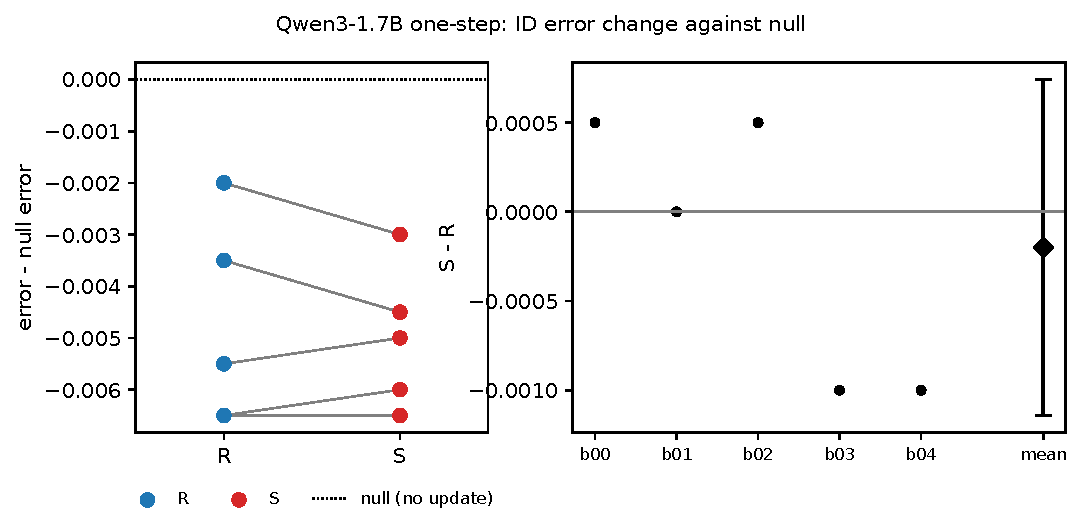
\includegraphics[width=0.82\linewidth]{figures/one_step_selected_raw/qwen3-1.7b_error_eval_id.pdf}
\par\smallskip
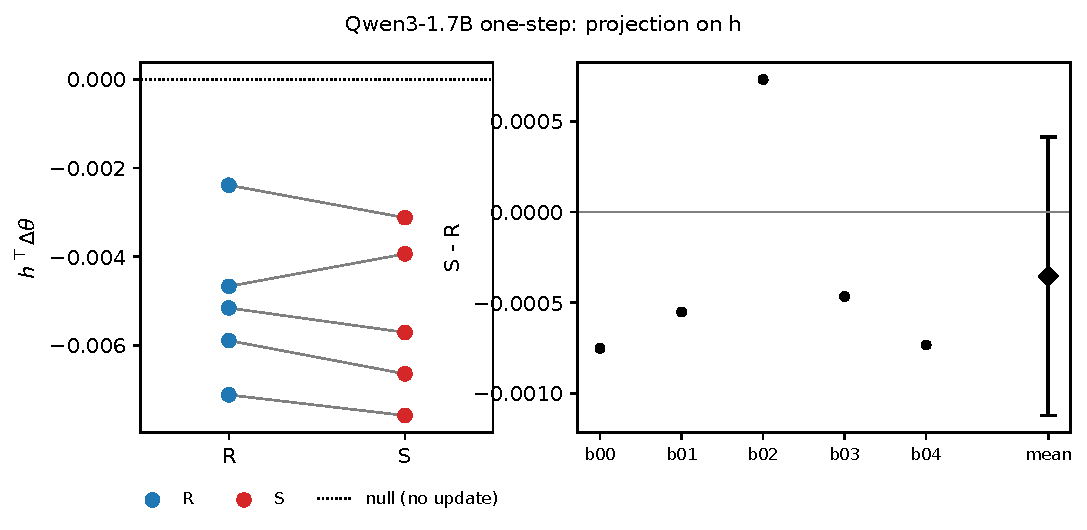
\includegraphics[width=0.82\linewidth]{figures/one_step_selected_raw/qwen3-1.7b_projection.pdf}
\caption{Original Qwen3-1.7B one-step ID error change against null
(top) and reference projection $h^T\Delta\theta$ (bottom), with five
paired blocks. The panels retain the run's own null as their reference.}
\label{fig:one-step-raw-qwen17}
\end{figure}

Both Qwen3-1.7B arms lower mean ID error relative to null, by
$0.0048/0.0050$ for $R/S$. The paired $S-R$ error contrast is
$-0.0002\pm0.0009$ and the projection contrast is
$-0.00035\pm0.00077$. Every block has
negative projection in both arms; none exhibits the theoretical
construction's opposite within-pair projection signs.

\begin{figure}[H]
\centering
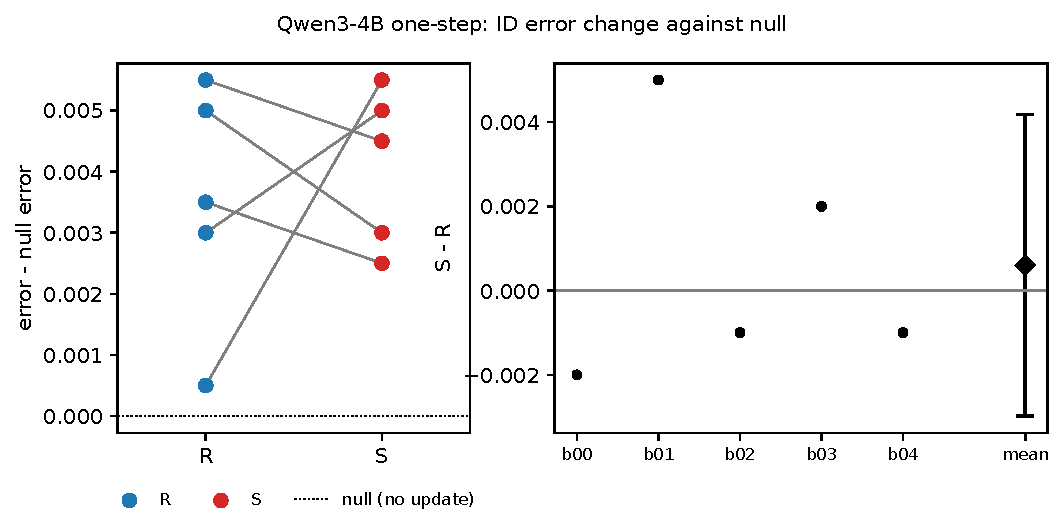
\includegraphics[width=0.82\linewidth]{figures/one_step_selected_raw/qwen3-4b_error_eval_id.pdf}
\par\smallskip
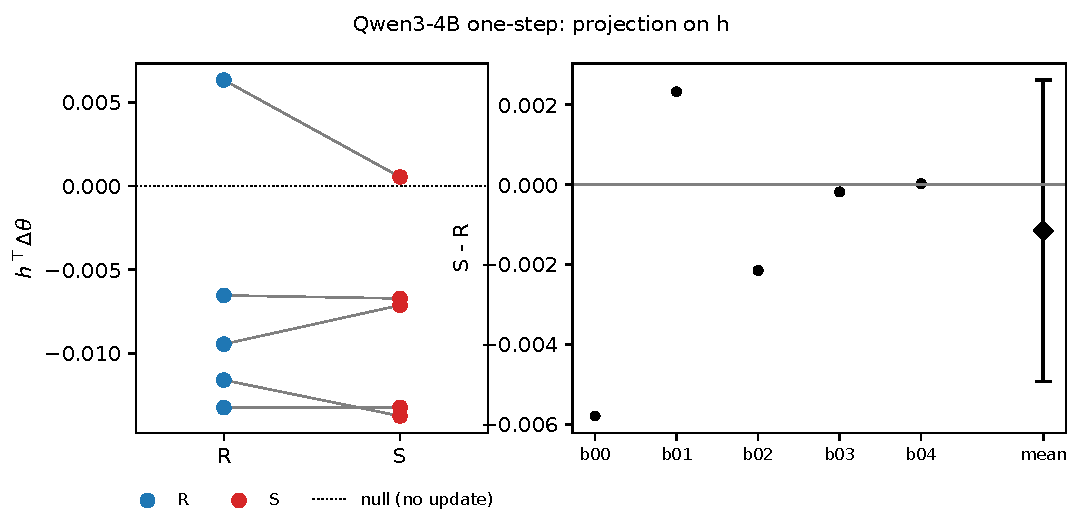
\includegraphics[width=0.82\linewidth]{figures/one_step_selected_raw/qwen3-4b_projection.pdf}
\caption{Original Qwen3-4B one-step ID error change against null
(top) and reference projection (bottom), with five paired blocks.
Error and projection are distinct outcomes and use separate scales.}
\label{fig:one-step-raw-qwen4}
\end{figure}

For Qwen3-4B, mean ID error increases by $0.0035/0.0041$ for $R/S$
despite negative mean projections. The paired contrasts are
$0.0006\pm0.0036$ for error and $-0.00115\pm0.00377$ for
projection. Block \texttt{b00} has positive
projection in both arms and the other four have negative projection
in both. A negative mean projection therefore does not certify
ID accuracy improvement.

\begin{figure}[H]
\centering
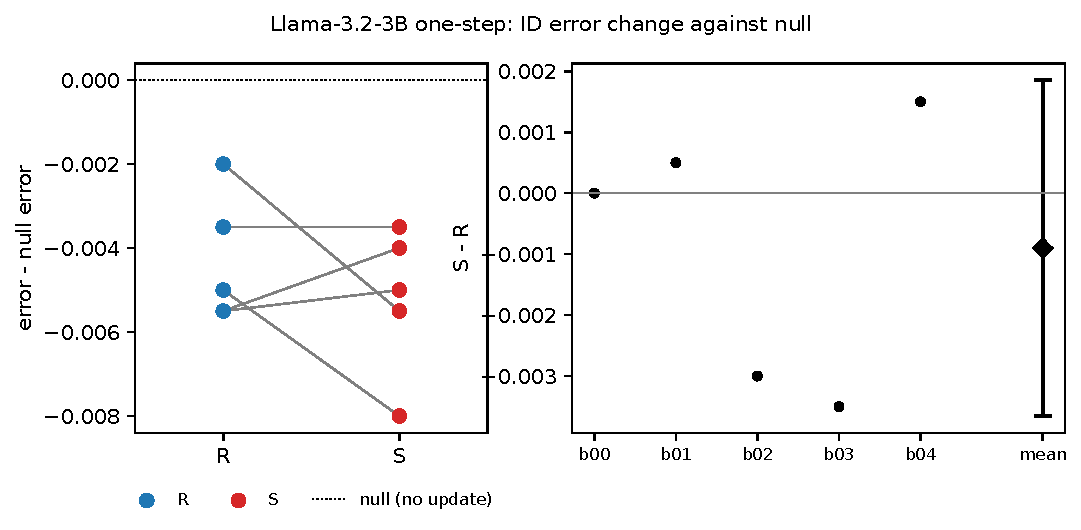
\includegraphics[width=0.82\linewidth]{figures/one_step_selected_raw/llama3.2-3b_error_eval_id.pdf}
\par\smallskip
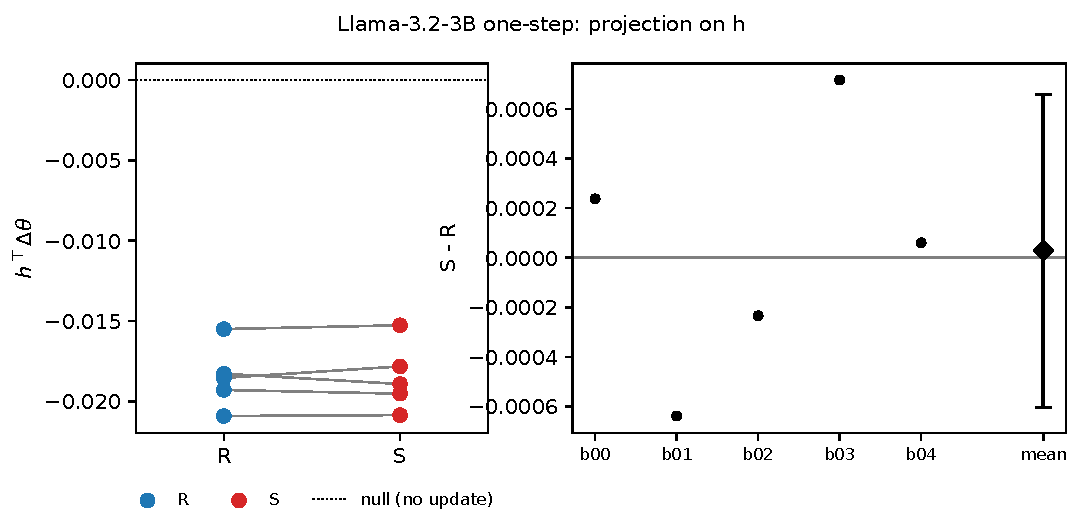
\includegraphics[width=0.82\linewidth]{figures/one_step_selected_raw/llama3.2-3b_projection.pdf}
\caption{Original Llama-3.2-3B-Instruct one-step ID error change
against null (top) and reference projection (bottom), with five
paired blocks.}
\label{fig:one-step-raw-llama}
\end{figure}

The Llama arms lower mean ID error by $0.0043/0.0052$ for $R/S$.
Paired contrasts are $-0.0009\pm0.0028$ for error and
$0.00003\pm0.00063$ for projection.
Every block has negative projection in both arms. These findings
do not establish equivalence of the arms or a within-pair directional
separation.
\endgroup


\paragraph{Validation and limits.}
Independent count-based checks reproduce the checkpoint metrics,
matching constraints, training and audit statistics, and paired contrasts
in the tables and figures. The figures preserve the underlying
observations and uncertainty. For these earlier exports, raw held-out answers,
adapter weights, and reference tensors are unavailable, so validation does
not include independent held-out rejudging, checkpoint reloading,
or tensor-level gradient recomputation. Qwen3-4B audited responses are
rejudged separately in Appendix~\ref{app:qwen4b-four-round}.
Run-specific baselines and reused
pools also prevent interpreting model-to-model differences as a controlled
model-size effect. Neither the finite-budget audit nor these one-step
diagnostics directly validate the population theorem's auditing policy.


